\chapter{Results and Discussion}

This chapter discusses the exploratory data analysis of the collected traffic and weather data to identify seasonalities, disruptions, and correlations. It also discusses the experiments performed in building the prediction model, as well as its evaluation. The traffic data includes traffic conditions for the whole year of 2015. The weather data includes weather variables such as wind speed, wind gust, temperature, humidity, dew point, precipitation, visibility, pressure, cloud cover, heat index, and feels-like, for  the three years 2015 to 2017.

\section{Pattern Analysis}
%%%%%%%%%%
\subsection{Connected Road Segments}
To be able to identify if there is a direct relationship between connected road segments, we first perform an initial correlation on their traffic for all working days in one month. Figure \ref{figure_traffic_roxas_corr} illustrates the correlation heatmap of the traffic of road segments in Roxas Boulevard. From this, we could observe a consistent strong relationship between each road. 


\begin{figure}[!t] 
\centering
    \centering
      \captionsetup{justification=centering}
    \subfloat[Southbound]{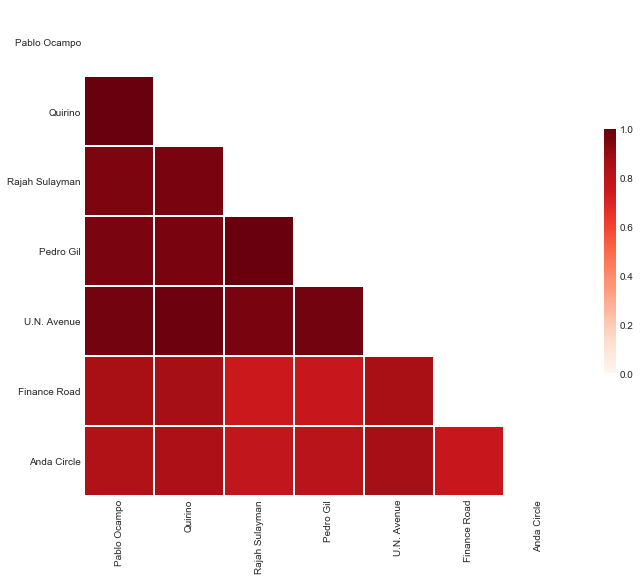
\includegraphics[width=0.5\textwidth]{figures/figure_traffic_roxas_sb_corr.png}\label{figure_traffic_roxas_sb_corr}}
    \hfill
    \subfloat[Northbound]{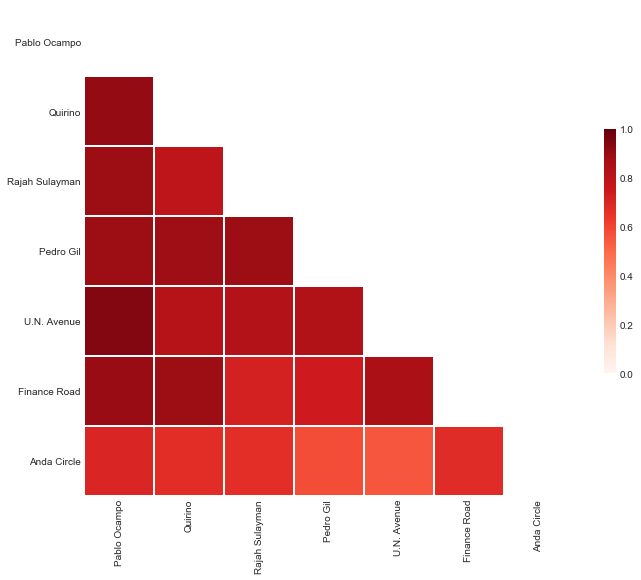
\includegraphics[width=0.5\textwidth]{figures/figure_traffic_roxas_nb_corr.png}\label{figure_traffic_roxas_nb_corr}}
    \caption{Correlation heatmap of traffic for both southbound and northbound of Roxas Boulevard}

    \label{figure_traffic_roxas_corr}
\end{figure}

This strong relationship remains true with the traffic for both southbound and northbound for Espana (see Figure \ref{figure_traffic_espana_corr}). Compared with Roxas Boulevard, however, there are certain road segments in Espana that have relatively weak relationship with its nearby road segments.


\begin{figure}[!t] 
\centering
    \centering
      \captionsetup{justification=centering}
    \subfloat[Southbound]{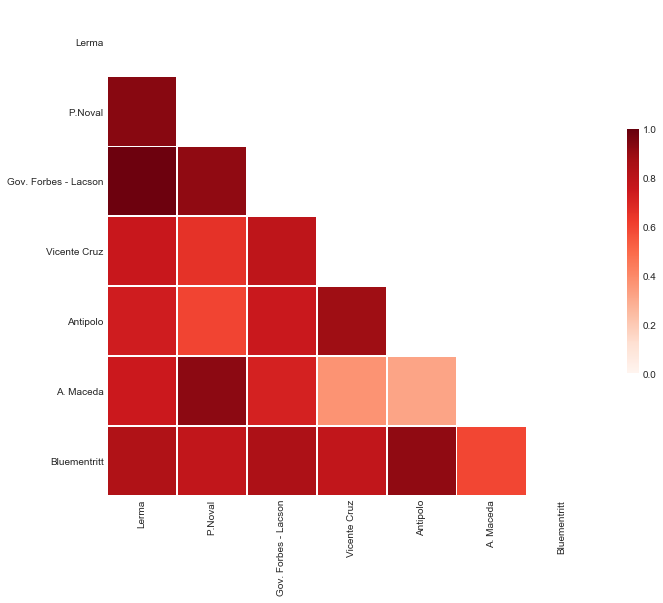
\includegraphics[width=0.5\textwidth]{figures/figure_traffic_espana_sb_corr.png}\label{figure_traffic_espana_sb_corr}}
    \hfill
    \subfloat[Northbound]{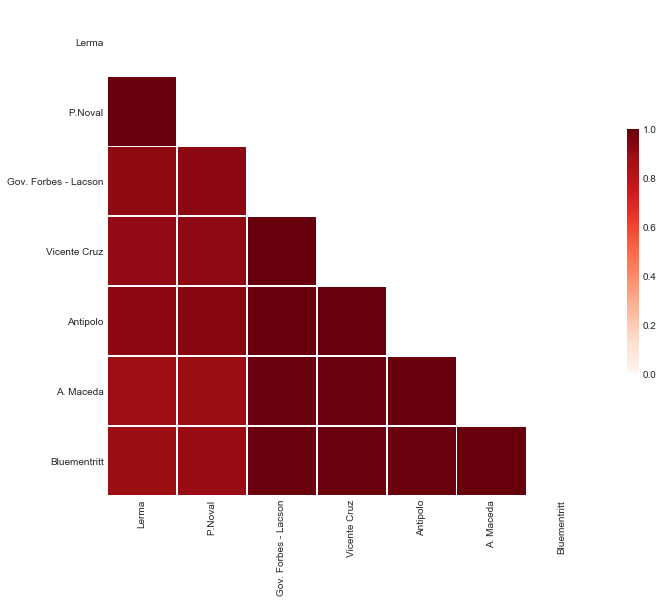
\includegraphics[width=0.5\textwidth]{figures/figure_traffic_espana_nb_corr.png}\label{figure_traffic_espana_nb_corr}}
    \caption{Correlation heatmap of traffic for both southbound and northbound of Espana}

    \label{figure_traffic_espana_corr}
\end{figure}


After analyzing the pattern of an individual road segment, we now analyze it as a part of a road. Exploring the working day traffic of all road segments in Roxas Boulevard in one month, it could be observed that there is an intensity relationship between these southbound road segments such that their peaks remain the same yet their intensity differs (see Figure \ref{figure_traffic_roxas}). This is also the case in the northbound of the road segments in Roxas Boulevard. The intense traffic of Pablo Ocampo is carried over to Quirino in a similar intensity yet continuously decays as we go further to Anda Circle.

\begin{figure}[!t] 
\centering
    \centering
      \captionsetup{justification=centering}
    \subfloat[Southbound]{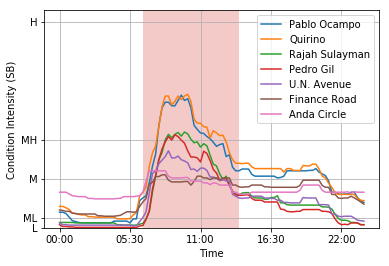
\includegraphics[width=0.5\textwidth]{figures/figure_traffic_roxas_sb.png}\label{figure_traffic_roxas_sb}}
    \hfill
    \subfloat[Northbound]{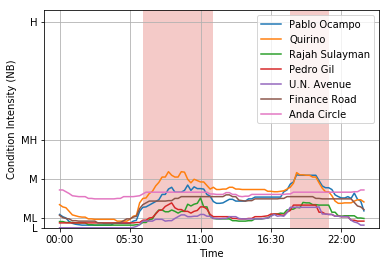
\includegraphics[width=0.5\textwidth]{figures/figure_traffic_roxas_nb.png}\label{figure_traffic_roxas_nb}}
    \caption{Daily average of all working days in one month in all road segments in Roxas Boulevard showing its intensity relationship}

    \label{figure_traffic_roxas}
\end{figure}




Likewise, in road segments of Espana, it follows a similar trend (see Figure \ref{figure_traffic_espana}). The intensity of the traffic at the northbound of Blumentritt rises as we approach Antipolo then decays as we go further to Lerma.


\begin{figure}[!t] 
\centering
    \centering
      \captionsetup{justification=centering}
    \subfloat[Southbound]{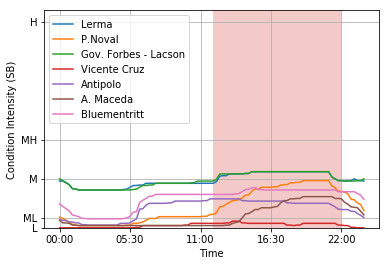
\includegraphics[width=0.5\textwidth]{figures/figure_traffic_espana_sb.png}\label{figure_traffic_espana_sb}}
    \hfill
    \subfloat[Northbound]{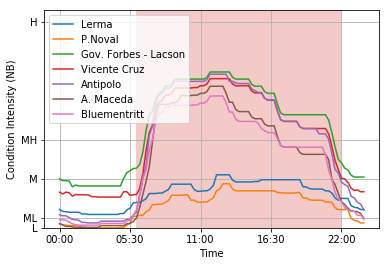
\includegraphics[width=0.5\textwidth]{figures/figure_traffic_espana_nb.png}\label{figure_traffic_espana_nb}}
    \caption{Daily average of all working days in one month in all road segments in Espana showing its intensity relationship}

    \label{figure_traffic_espana}
\end{figure}

In summary, in consideration with the strong correlation between connected road segments, and dynamic traffic intensity, it can be concluded that the road segments which can generally describe the other road segments in the same road are Pablo Ocampo, for Roxas Boulevard, and Antipolo, for Espana.



\subsection{Traffic Analysis}

Analyzing the autocorrelation plot of traffic (see Figure \ref{figure_autocorr_week}) for both Pablo Ocampo and Antipolo, it could be observed that in spite of its daily pattern, its succeeding days are loosely correlated with the present one. Notably, it is noticeable how the seasonality the day before (e.g. similarity of a Tuesday observation with yesterday’s Monday) and the week before (e.g. similarity of a Monday observation with last week's Monday) are relatively stronger compared with the other days (e.g. 2 days ago, 3 days ago).

\begin{figure}[!t] 
\centering
    \centering
      \captionsetup{justification=centering}
    \subfloat[Pablo Ocampo (Southbound)]{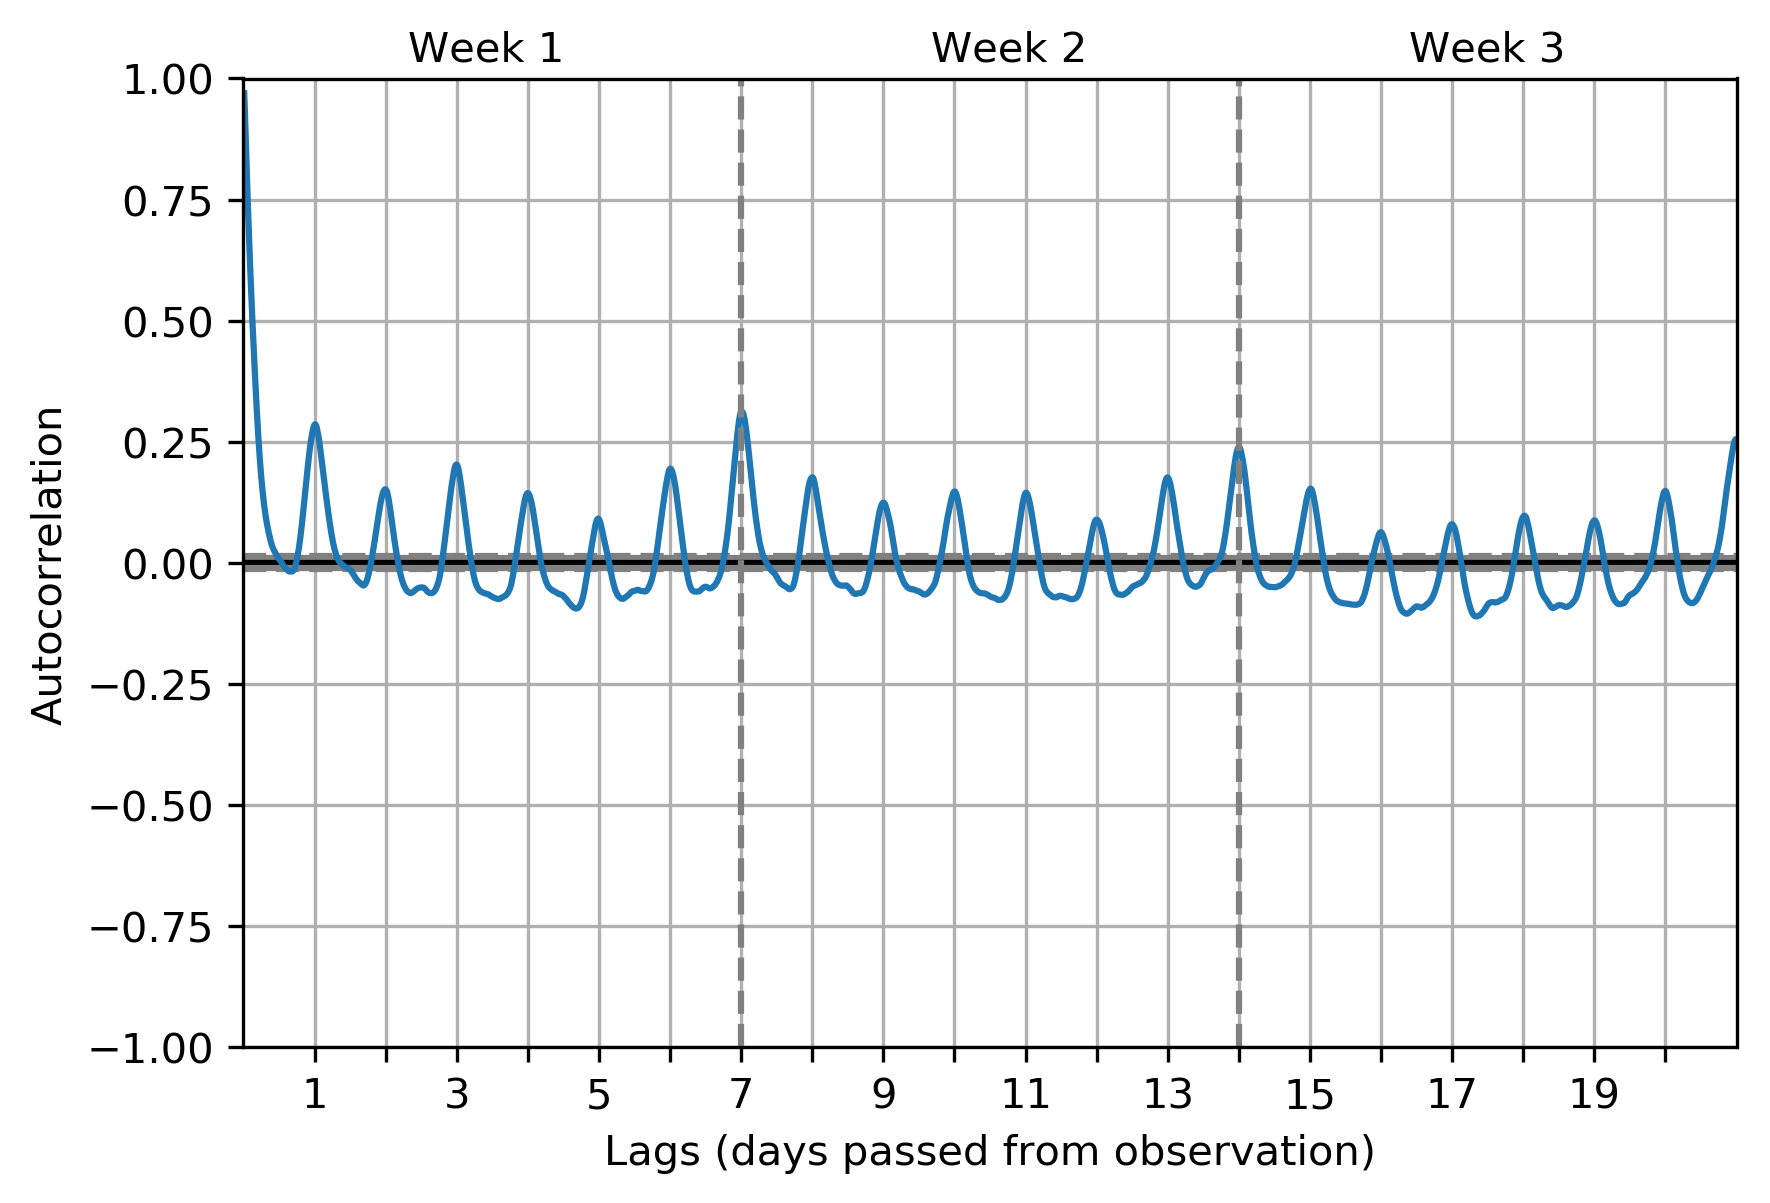
\includegraphics[width=0.5\textwidth]{figures/figure_autocorr_pocampo.png}\label{figure_autocorr_pocampo}}
    \hfill
    \subfloat[Antipolo (Northbound)]{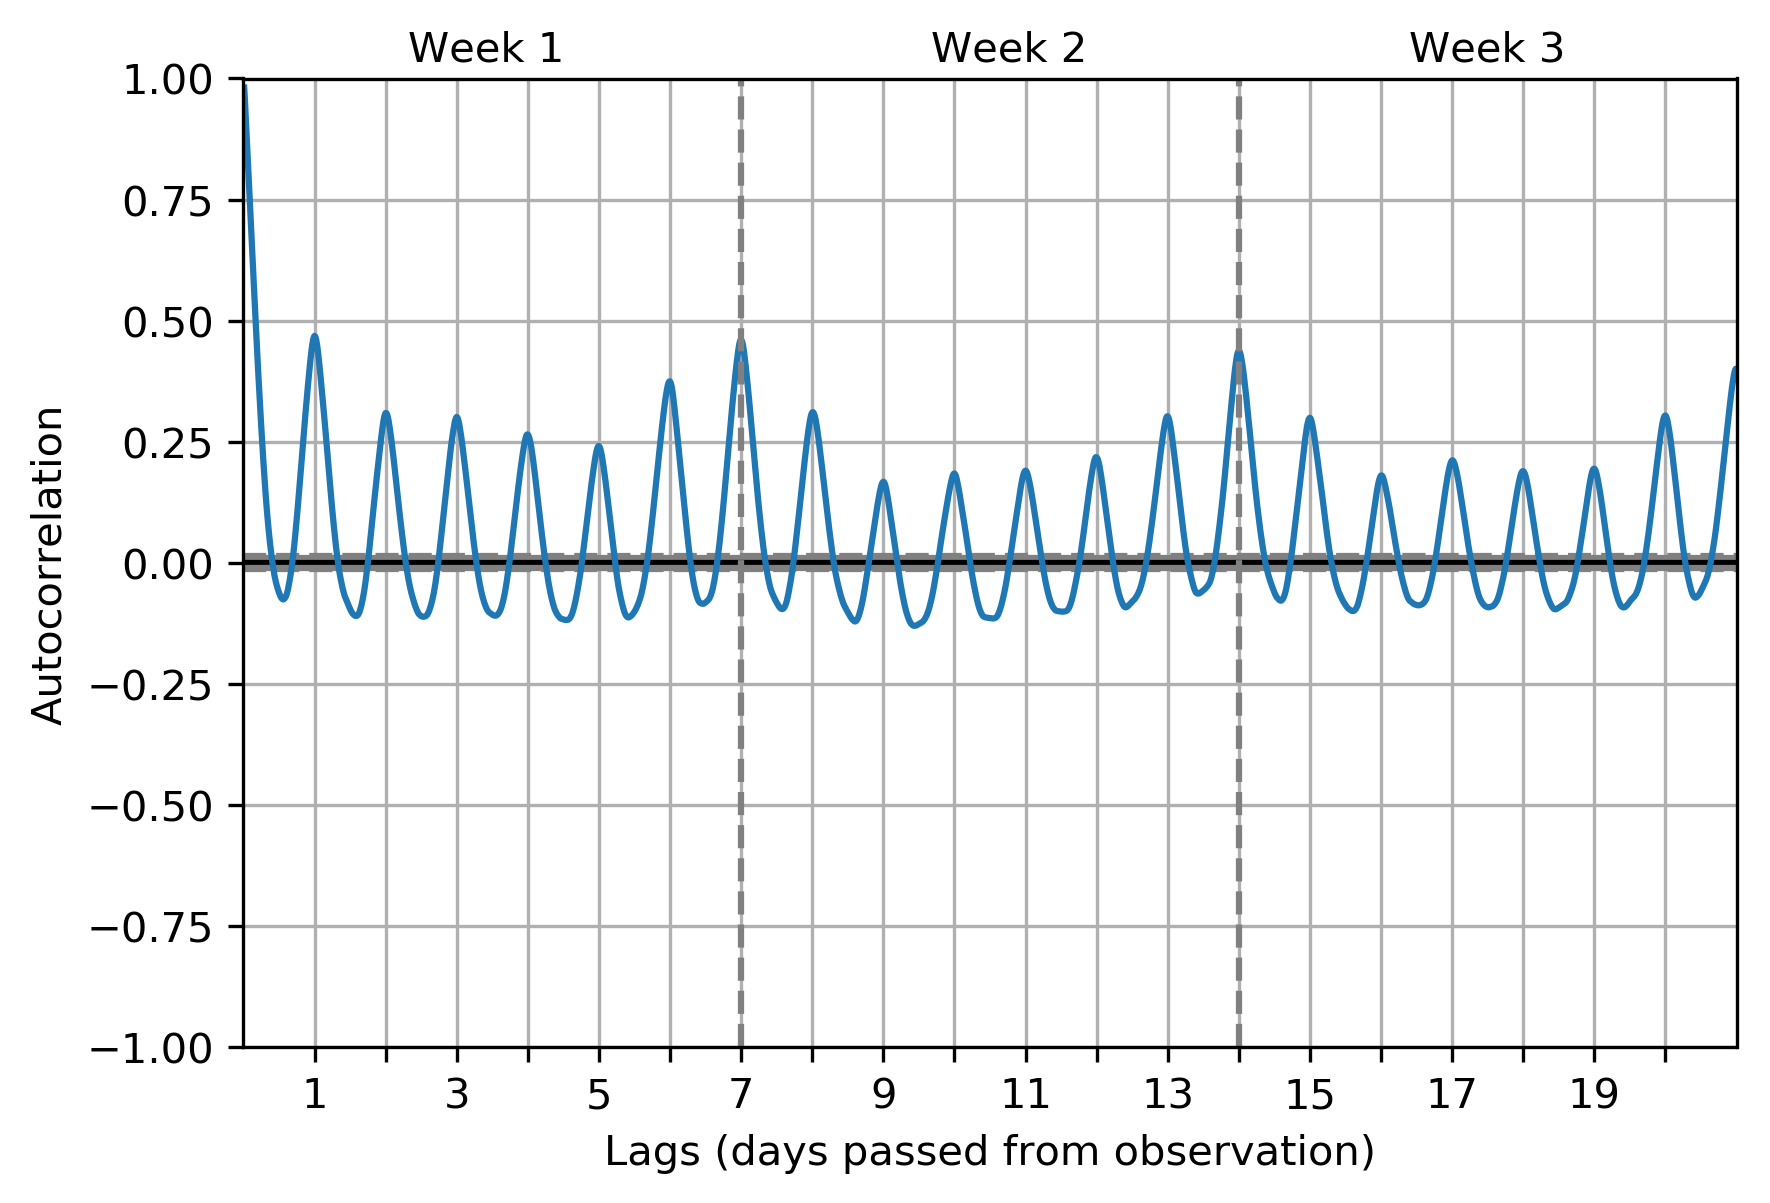
\includegraphics[width=0.5\textwidth]{figures/figure_autocorr_antipolo.png}\label{figure_autocorr_antipolo}}
    \caption{Autocorrelation plot of (a) Pablo Ocampo and (b) Antipolo revealing its daily and weekly seasonality}

    \label{figure_autocorr_week}
\end{figure}

\begin{figure}[!t] 
\centering
    \centering
      \captionsetup{justification=centering}
    \subfloat[Pablo Ocampo (Southbound)]{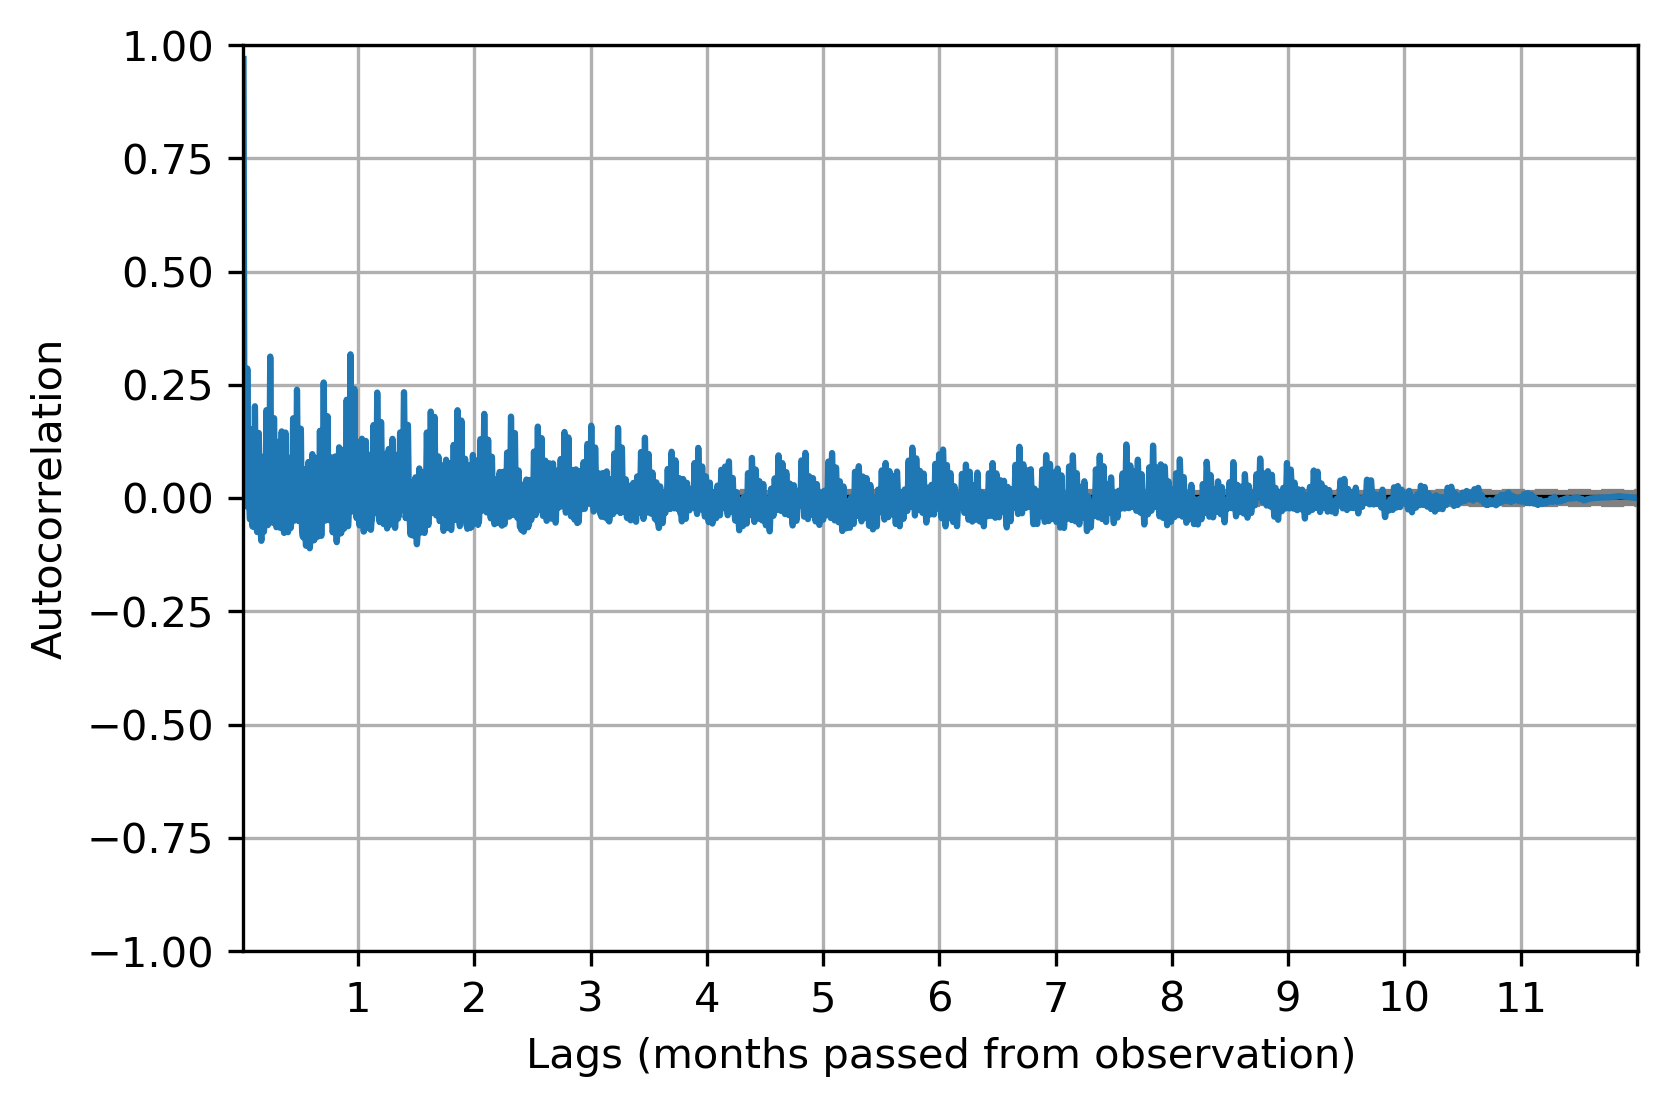
\includegraphics[width=0.5\textwidth]{figures/figure_autocorr_traffic_month_pocampo.png}\label{figure_autocorr_traffic_month_pocampo}}
    \hfill
    \subfloat[Antipolo (Northbound)]{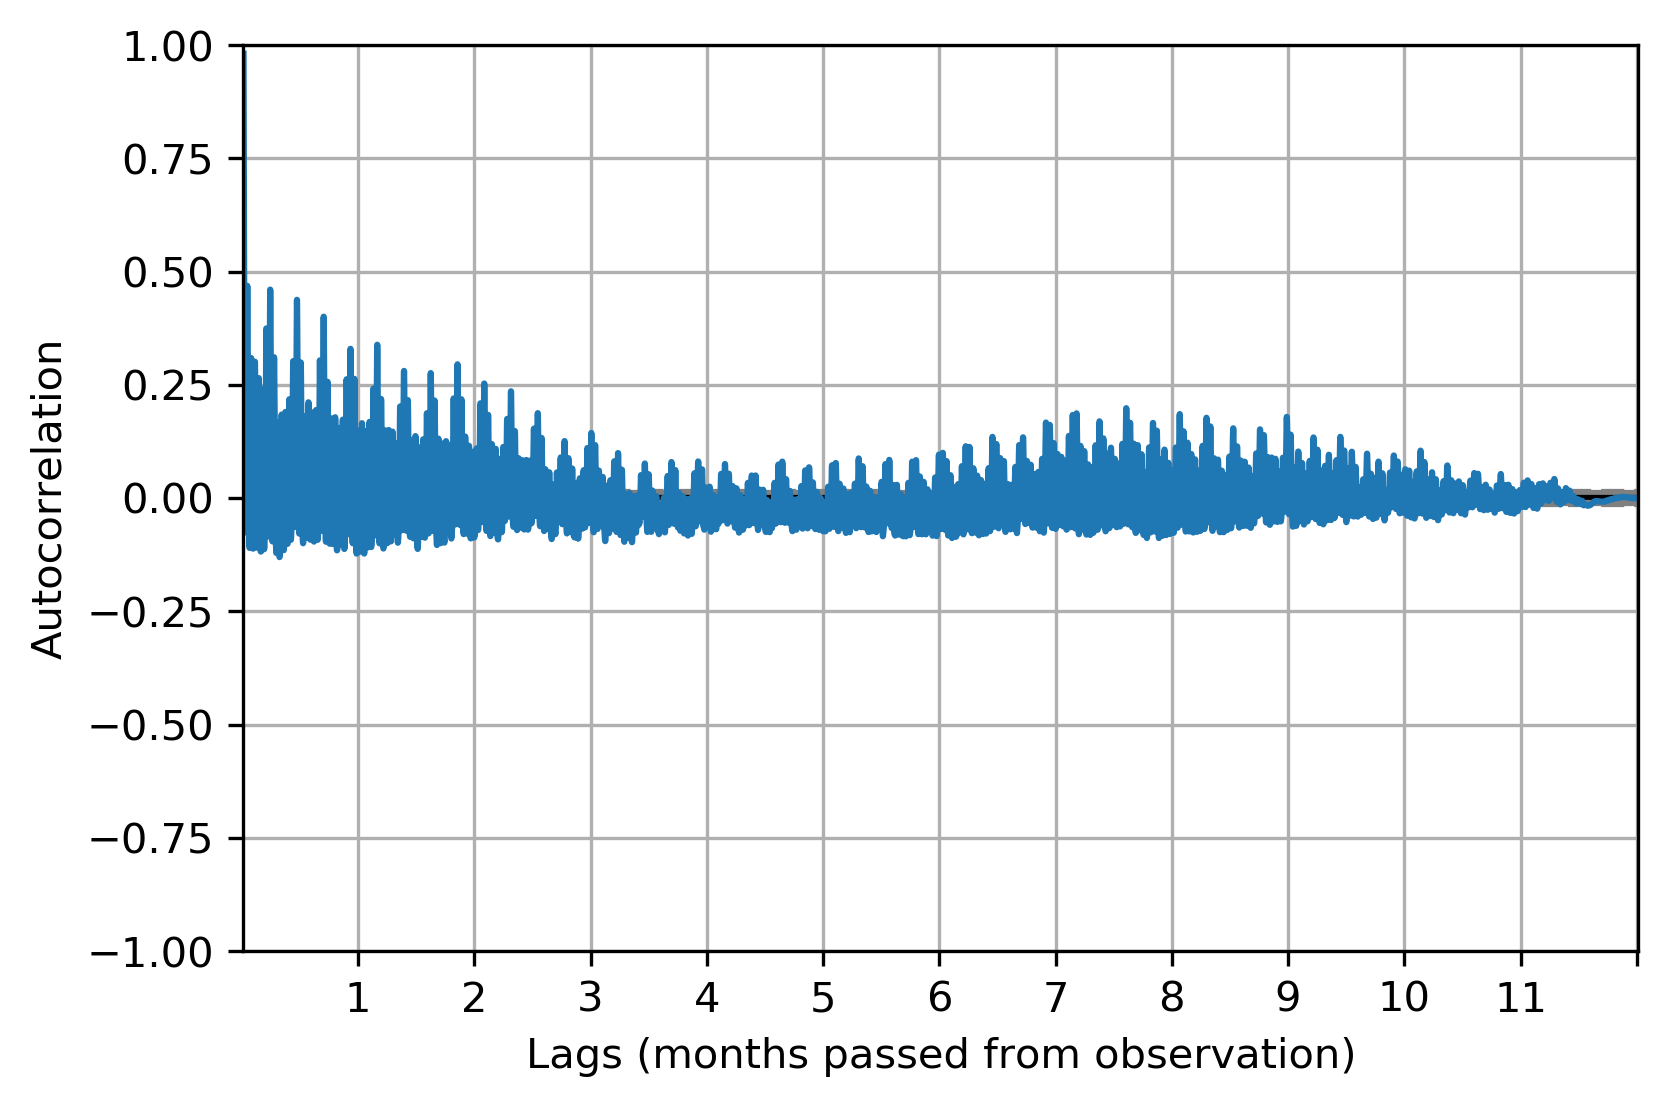
\includegraphics[width=0.5\textwidth]{figures/figure_autocorr_traffic_month_antipolo.png}\label{figure_autocorr_traffic_month_antipolo}}
    \caption{Autocorrelation plot of (a) Pablo Ocampo and (b) Antipolo showing a decaying weekly seasonality}

    \label{figure_autocorr_traffic_month}
\end{figure}

Viewing their pattern in a longer term (e.g. month-long), nevertheless, its weekly pattern becomes looser as months go by (see Figure \ref{figure_autocorr_traffic_month}). In other words, traffic patterns must not be analyzed by segmenting it by month. Instead, it must be analyzed weeks prior to the current observation as mutations in the traffic pattern may just be caused by a change in pattern carrying over to the succeeding days.


 
\subsubsection{Day Before}

Comparing the average traffic between working days and non-working days in one month, we could see a significant difference in terms of intensity and pattern (see Figure \ref{figure_workingday_comparison}). Majority of intense traffic occurs at working days. Table \ref{table_traffic_cond_workingday} shows that heavy traffic consists 17.8\% and 35.3\% of the working day of Pablo Ocampo’s southbound and Antipolo’s northbound respectively, while having none during non-working days for both road segments. Moreover, light traffic consists only 30.5\% and 26.1\% of the working day traffic of Pablo Ocampo’s southbound and Antipolo’s northbound respectively, while it accounts for 73.7\% and 61.6\% of the non-working day traffic.


\begin{figure}[!t] 
\centering
    \centering
      \captionsetup{justification=centering}
    \subfloat[Pablo Ocampo (Southbound)]{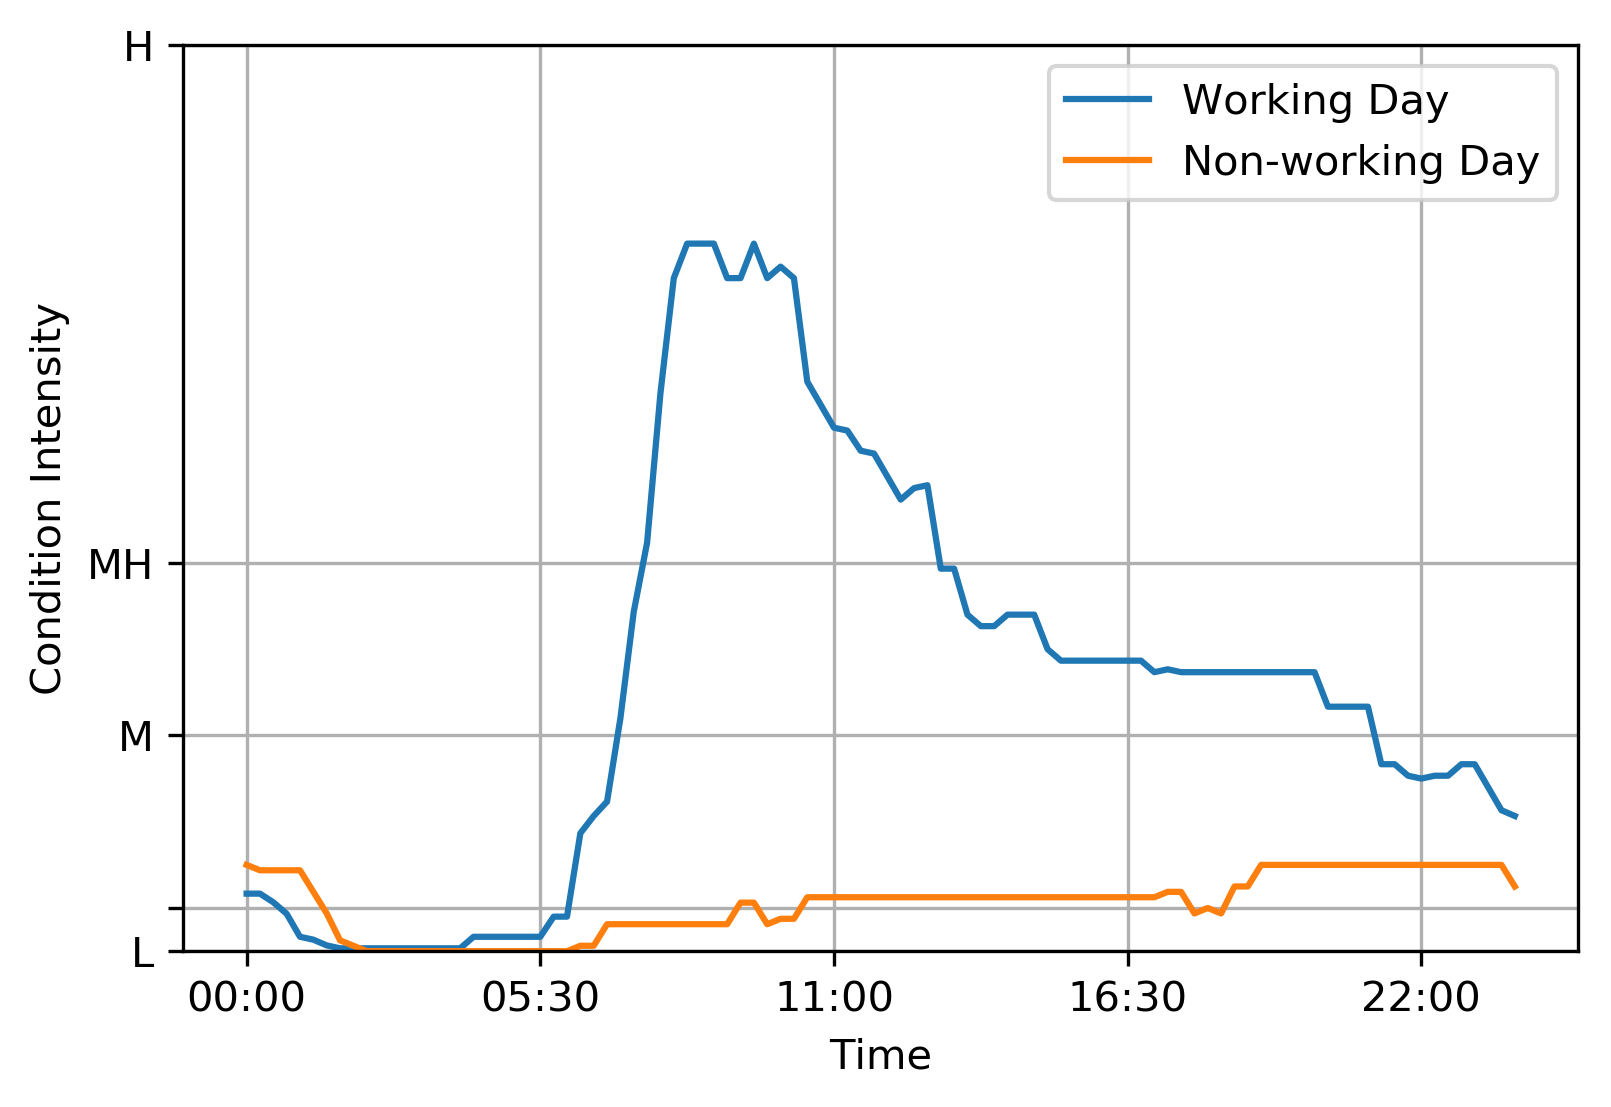
\includegraphics[width=0.5\textwidth]{figures/figure_workingday_comparison_pocampo.png}\label{figure_workingday_comparison_pocampo}}
    \hfill
    \subfloat[Antipolo (Northbound)]{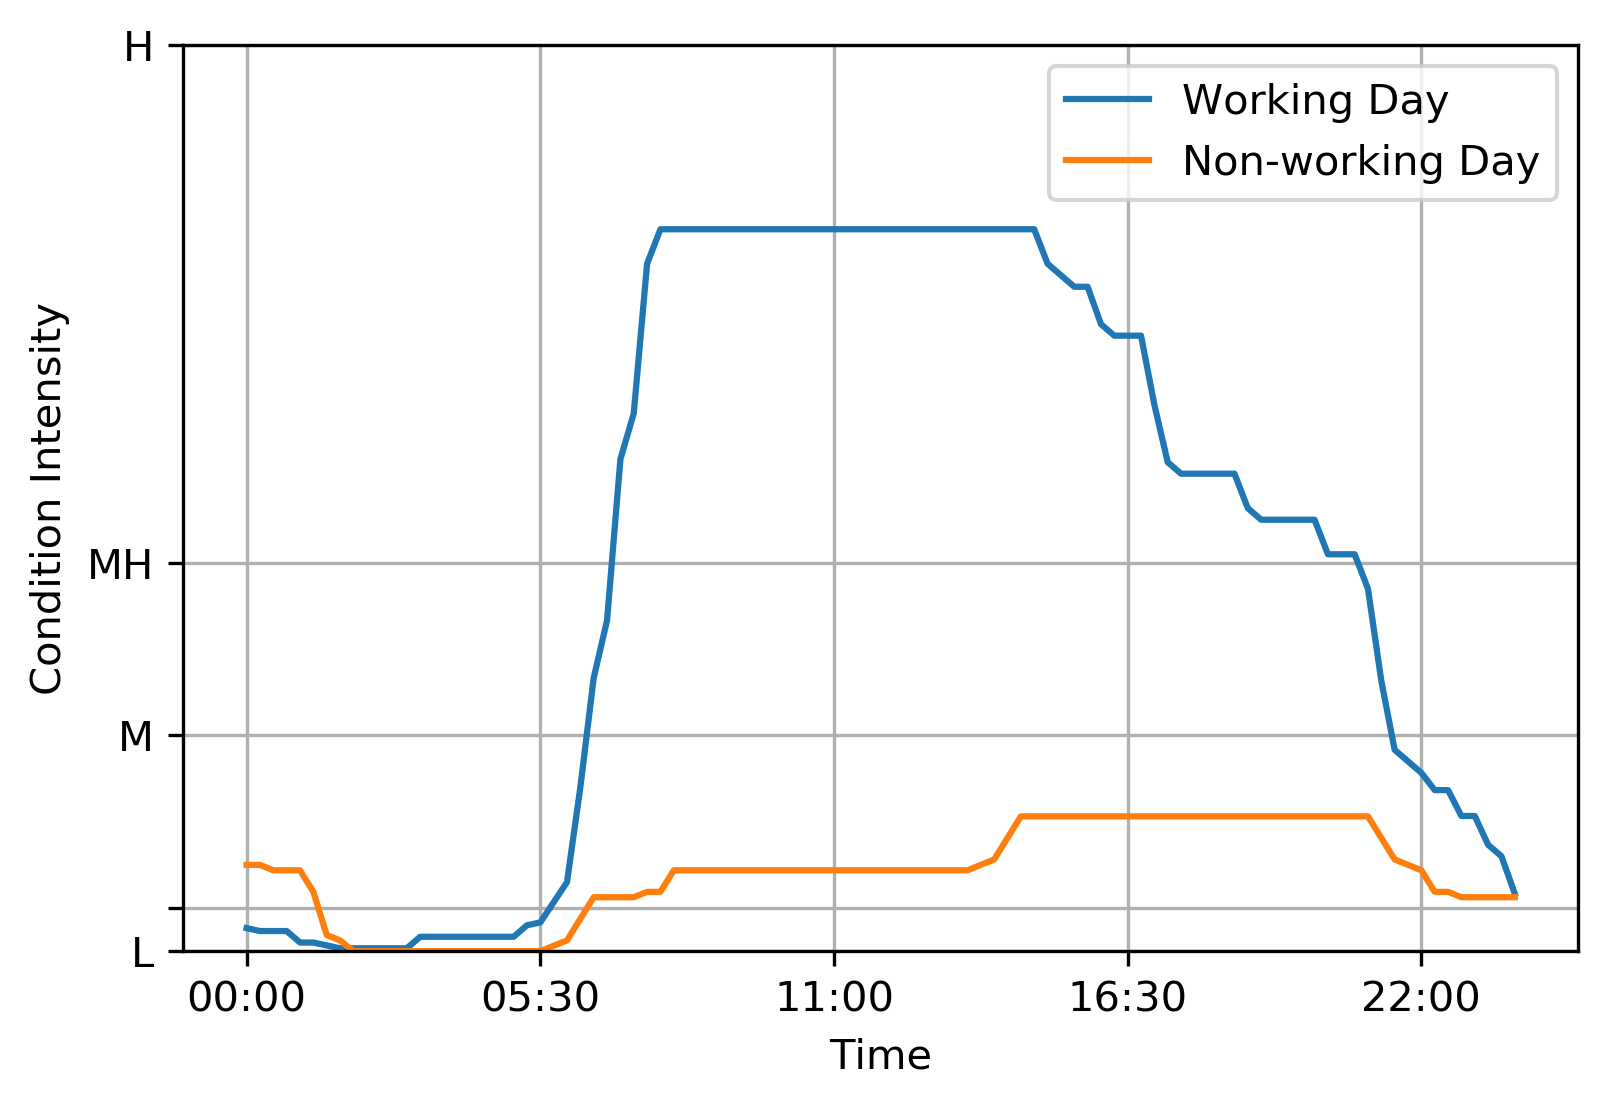
\includegraphics[width=0.5\textwidth]{figures/figure_workingday_comparison_antipolo.png}\label{figure_workingday_comparison_antipolo}}
    \caption{Comparison of the average traffic of (a) Pablo Ocampo’s southbound and (b) Antipolo’s northbound  in one month between working and non-working revealing the lack of intense traffic for non-working days}

    \label{figure_workingday_comparison}
\end{figure}



%%%%%%%%%%%%%%%%%%%%%%%%%%%%%%%%%%%%%%%%%%%%%
%INSERT GELO CHANGES
%%%%%%%%%%%%%%%%%%%%%%%%%%%%%%%%%%%%%%%%%%%%%
\begin{table}[!t]
\centering
\caption{Comparison of traffic condition distribution between working and non-working}
\label{table_traffic_cond_workingday}
\begin{tabular}{|l|r|r|r|r|}
\hline
 & \multicolumn{2}{c|}{\textbf{\begin{tabular}[c]{@{}c@{}}Pablo Ocampo\\ (Southbound)\end{tabular}}} & \multicolumn{2}{c|}{\textbf{\begin{tabular}[c]{@{}c@{}}Antipolo \\ (Northbound)\end{tabular}}} \\ \hline
\textbf{\begin{tabular}[c]{@{}l@{}}Traffic \\ Condition\end{tabular}} & \multicolumn{1}{r|}{\textbf{\begin{tabular}[c]{@{}r@{}}Working \\ Day\end{tabular}}} & \multicolumn{1}{r|}{\textbf{\begin{tabular}[c]{@{}r@{}}Non-working \\ Day\end{tabular}}} & \multicolumn{1}{r|}{\textbf{\begin{tabular}[c]{@{}r@{}}Working \\ Day\end{tabular}}} & \multicolumn{1}{r|}{\textbf{\begin{tabular}[c]{@{}r@{}}Non-working \\ Day\end{tabular}}} \\ \hline
\textbf{L} & 30.5\% & 73.7\% & 26.1\% & 61.6\% \\ \hline
\textbf{ML} & 6.1\% & 5.9\% & 5.0\% & 3.1\% \\ \hline
\textbf{M} & 41.4\% & 20.2\% & 31.3\% & 35.3\% \\ \hline
\textbf{MH} & 4.2\% & 0.3\% & 2.2\% & 0.0\% \\ \hline
\textbf{H} & 17.8\% & 0.0\% & 35.3\% & 0.0\% \\ \hline
\end{tabular}
\end{table}

%%%%%%%%%%%%%%%%%%%%%%%%%%%%%%%%%%%%%%%%%%%%%

This, in terms of trends, indicates that the working day traffic may follow the peak hour-driven traffic pattern. In this study, the researchers considered the mean of heavy and moderately heavy traffic as the threshold in detecting the peak hour (see Figure \ref{figure_peakhour}). Coming from nominal categorical data, however, there are instances when traffic changes its condition but only for a short while (see Figure \ref{figure_peakhour_problem}). With these problems present, discontinuous and false peak hours might be identified. Therefore, to alleviate these problems, an allowance threshold of 1 hour or 4 intervals is considered such that if there is a below-peak hour threshold condition change that occurred for only an hour or less, these would be recognized as part of the peak hour. Similarly, if an above-peak hour threshold condition change that occur for only an hour or less, these will not be recognized as part of the peak hour. The results of the improved peak hour detection is illustrated in Figure \ref{figure_peakhour_solution}.


\begin{figure}[!t] 
\centering
    \centering
      \captionsetup{justification=centering}
    \subfloat[Pablo Ocampo (Southbound)]{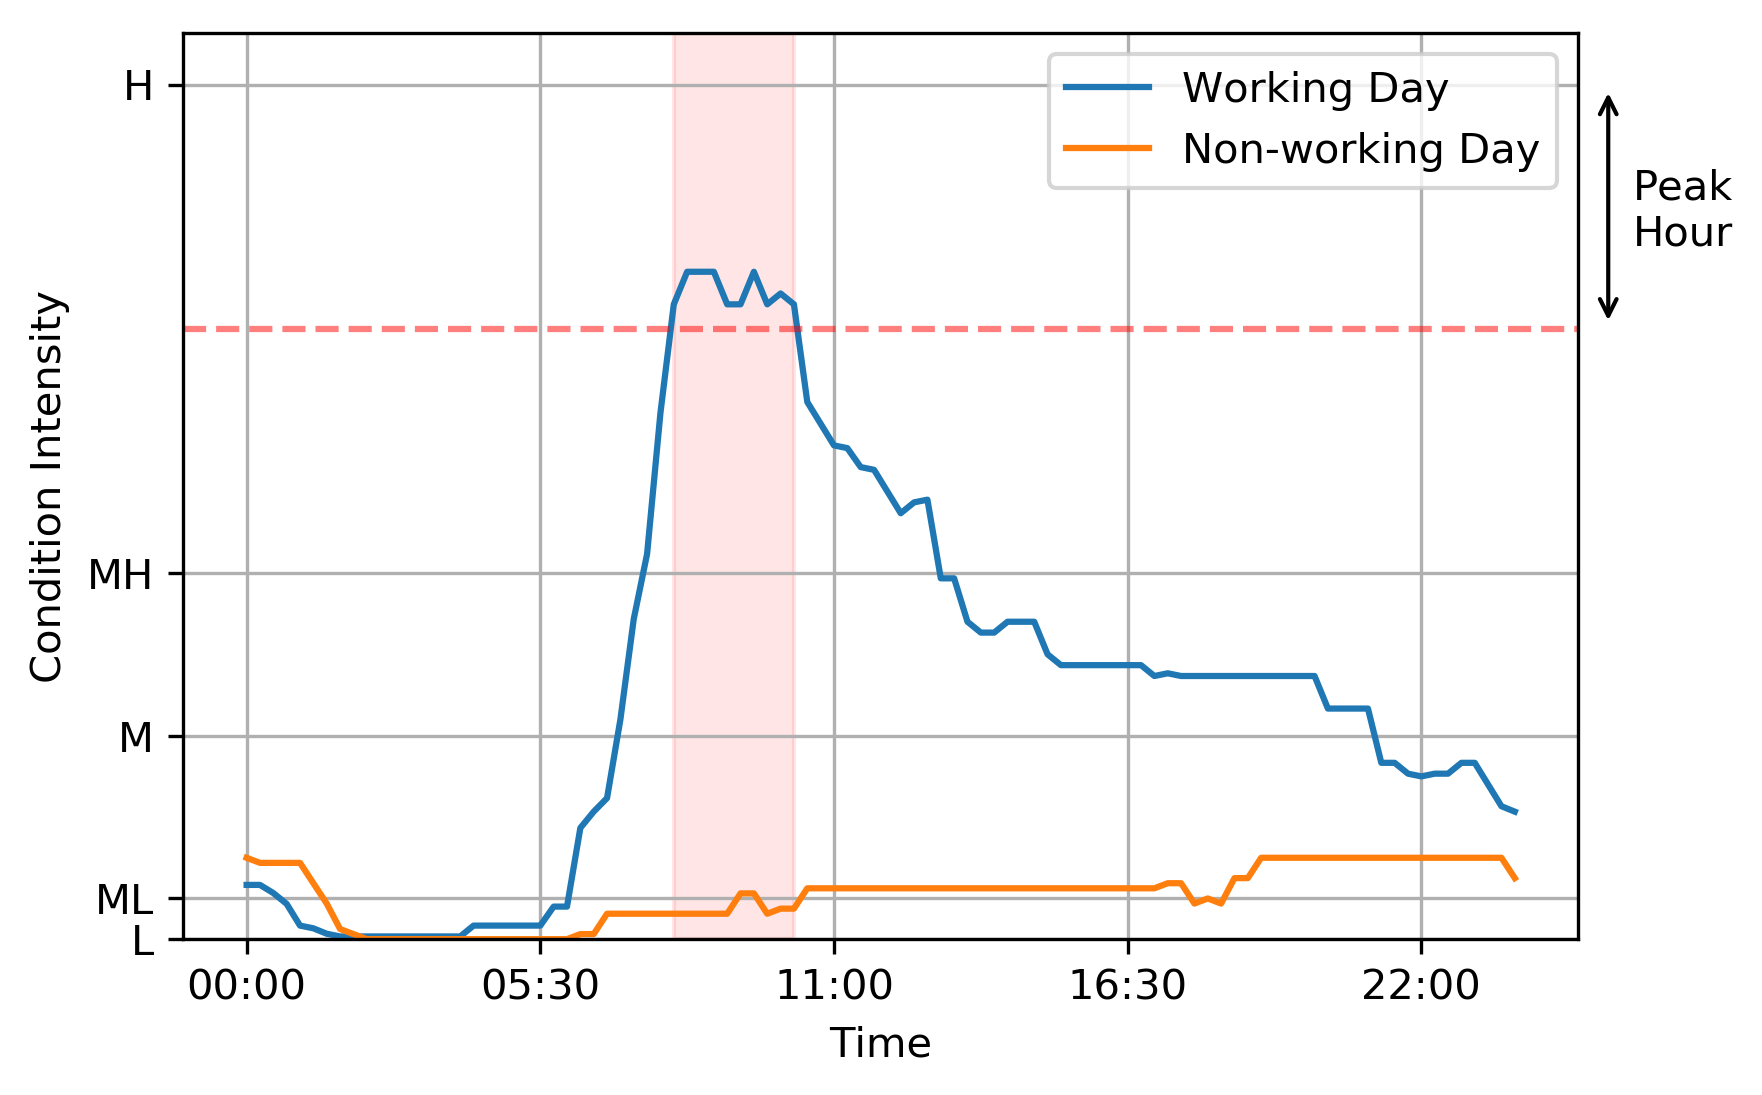
\includegraphics[width=0.5\textwidth]{figures/figure_peakhour_pocampo.png}\label{figure_peakhour_pocampo}}
    \hfill
    \subfloat[Antipolo (Northbound)]{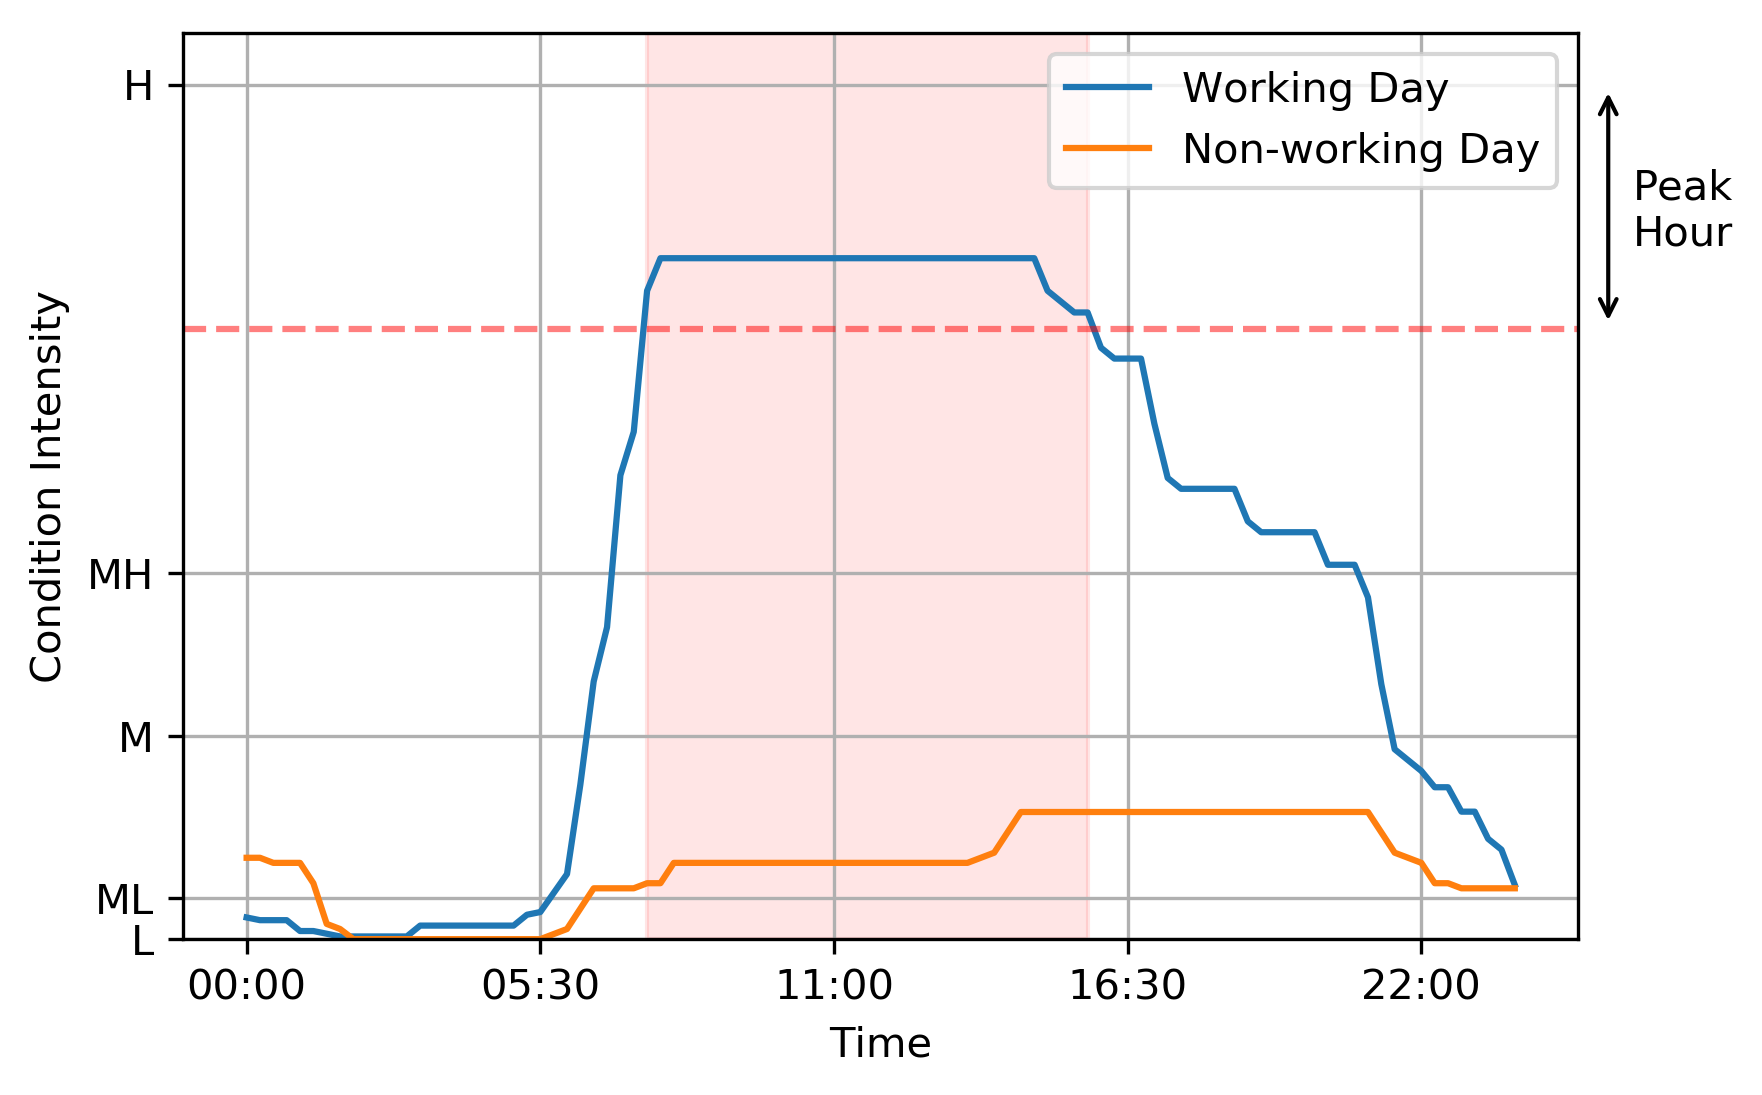
\includegraphics[width=0.5\textwidth]{figures/figure_peakhour_antipolo.png}\label{figure_peakhour_antipolo}}
    \caption{Comparison of peak hours of the average traffic of (a) Pablo Ocampo’s southbound and (b) Antipolo’s northbound  in one month between working and non-working}

    \label{figure_peakhour}
\end{figure}


\begin{figure}[!t] 
\centering
    \centering
      \captionsetup{justification=centering}
    \subfloat[Short-term below-peak hour threshold condition change]{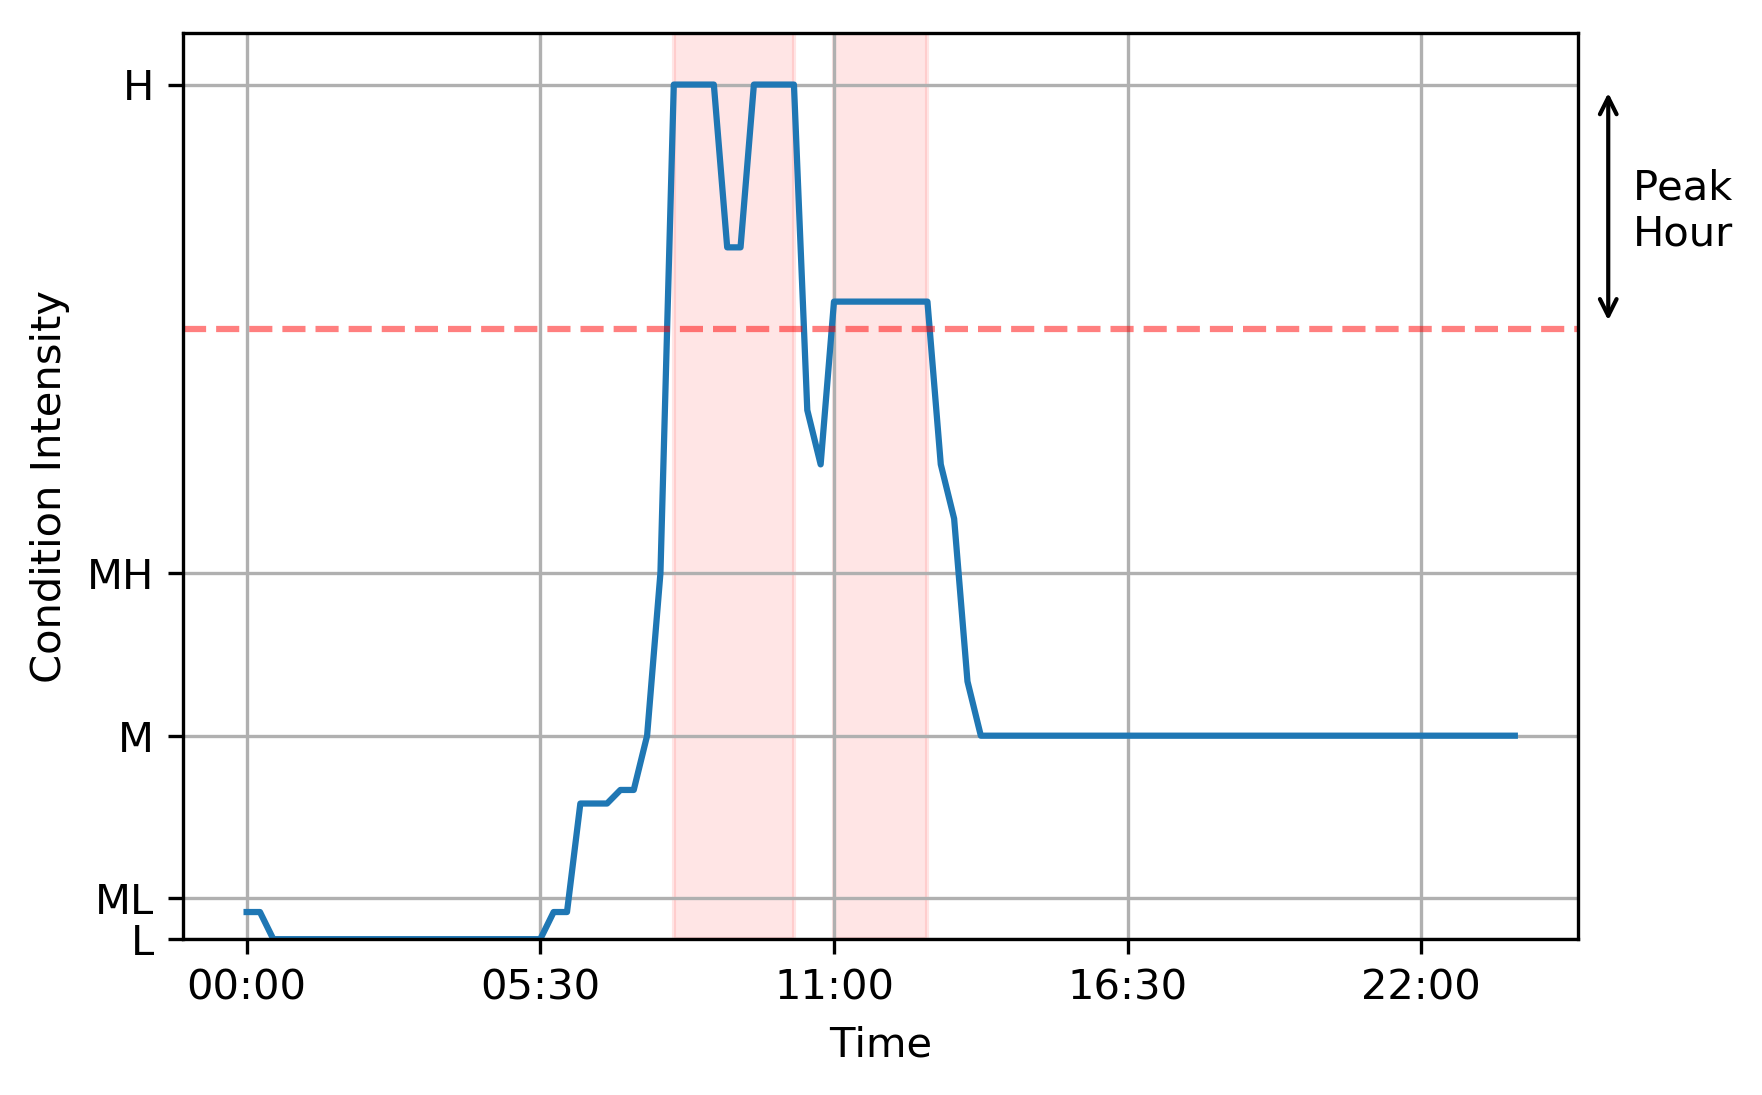
\includegraphics[width=0.5\textwidth]{figures/figure_peakhour_problem1.png}\label{figure_peakhour_problem1}}
    \hfill
    \subfloat[Short-term above-peak hour threshold condition change]{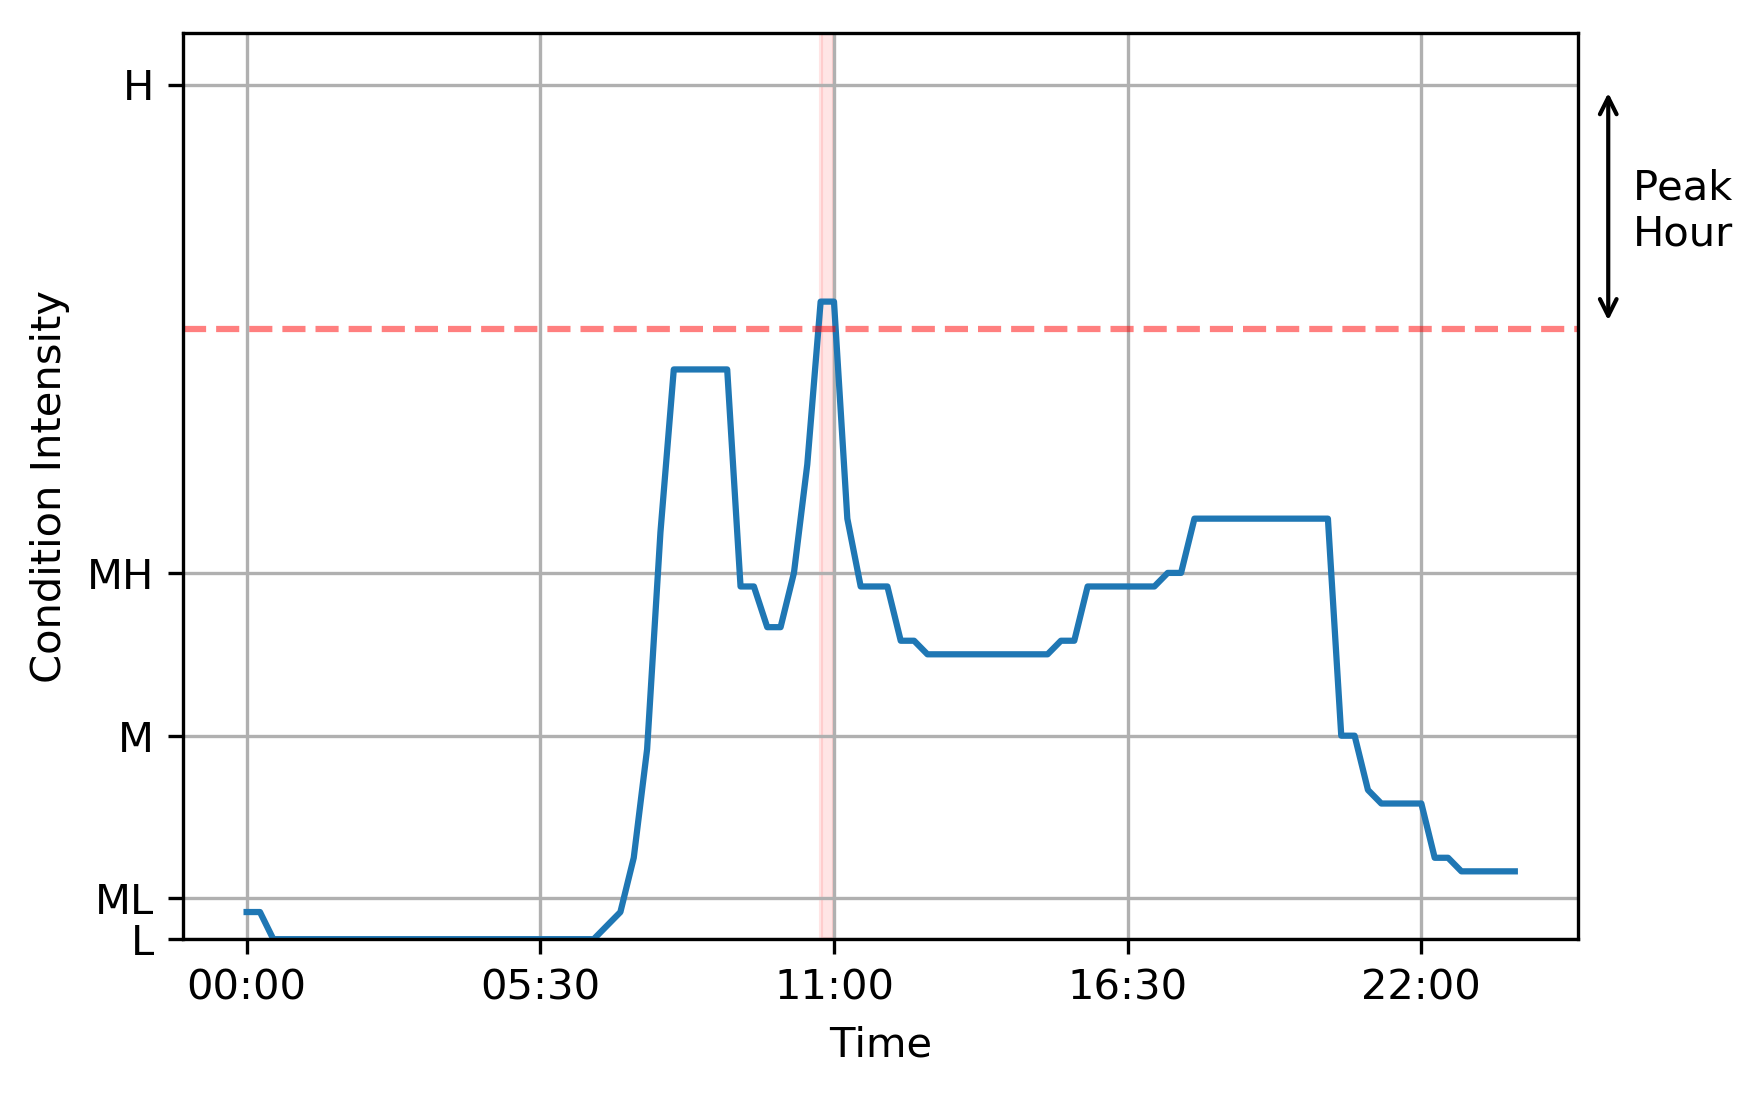
\includegraphics[width=0.5\textwidth]{figures/figure_peakhour_problem2.png}\label{figure_peakhour_problem2}}
    \caption{Examples of one-month average working day traffic of Pablo Ocampo’s southbound illustrating the issues in the peak hour detection in terms of short-term (a) below-peak hour and (b) above-peak hour condition change}

    \label{figure_peakhour_problem}
\end{figure}


\begin{figure}[!t] 
\centering
    \centering
      \captionsetup{justification=centering}
    \subfloat[Short-term below-peak hour threshold condition change]{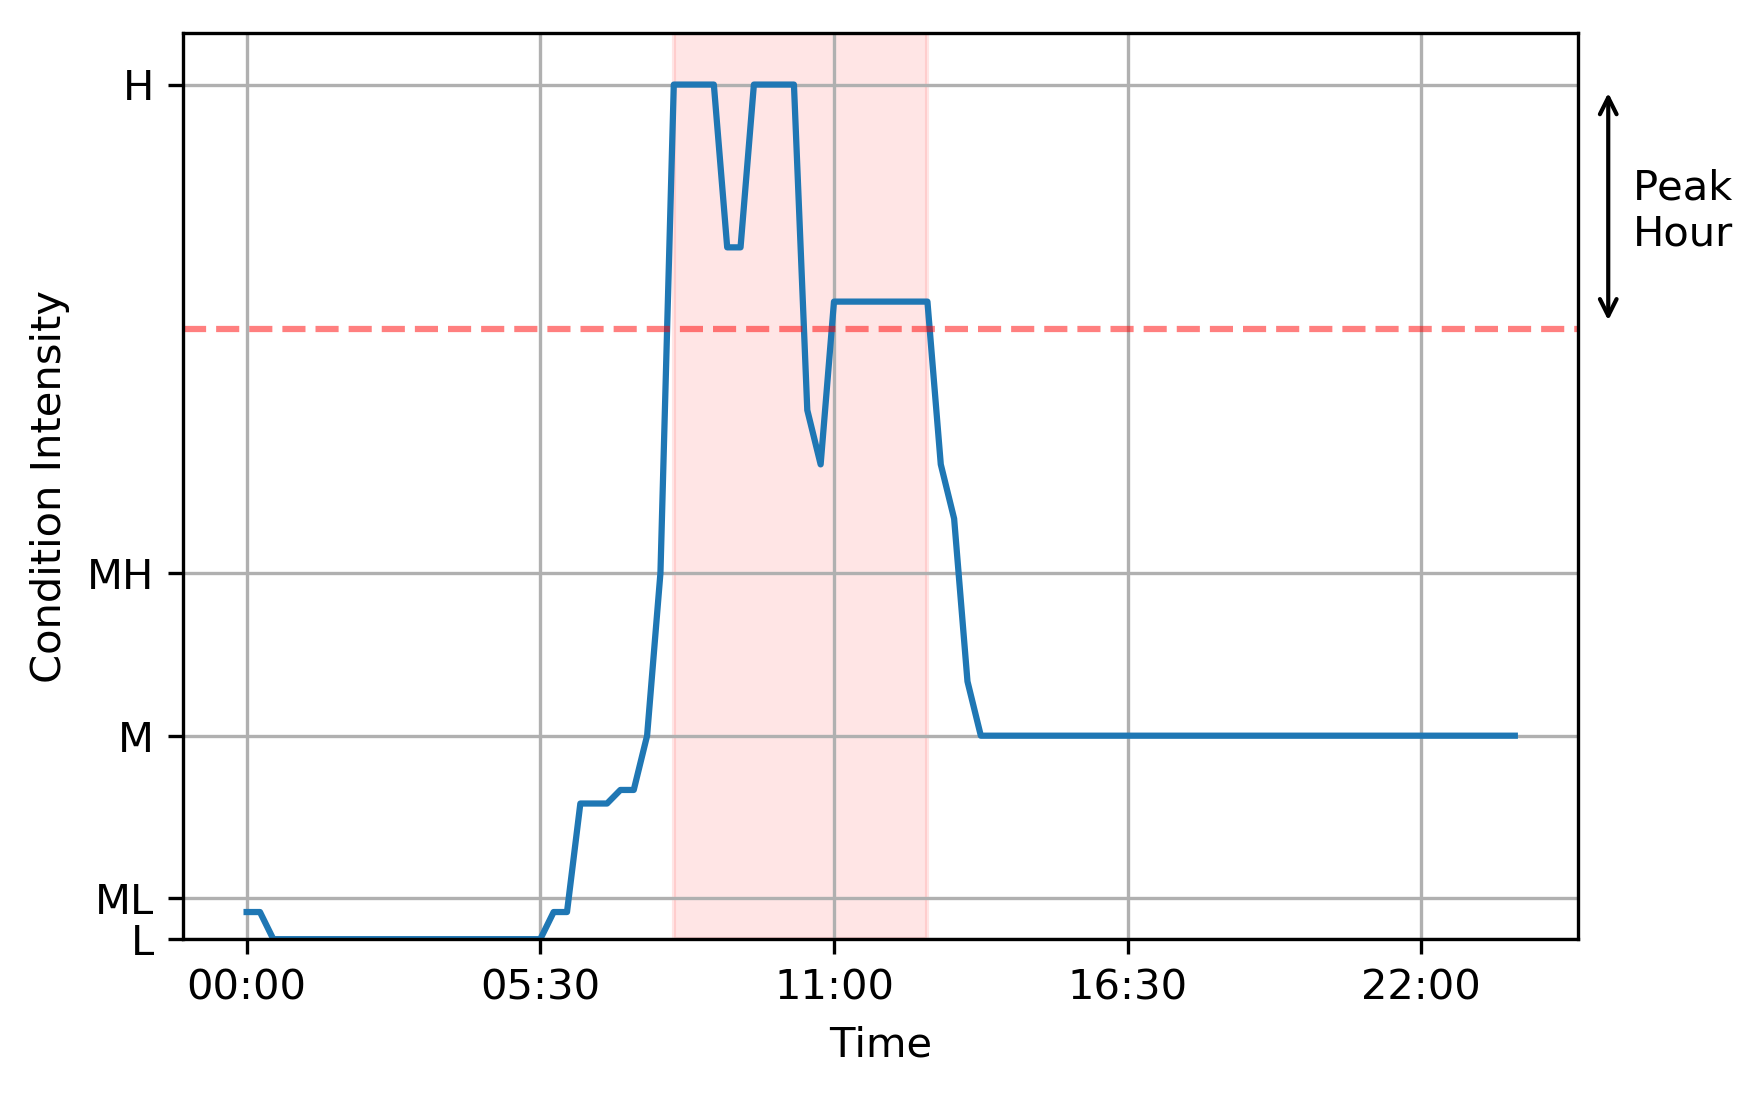
\includegraphics[width=0.5\textwidth]{figures/figure_peakhour_solution1.png}\label{figure_peakhour_solution1}}
    \hfill
    \subfloat[Short-term above-peak hour threshold condition change]{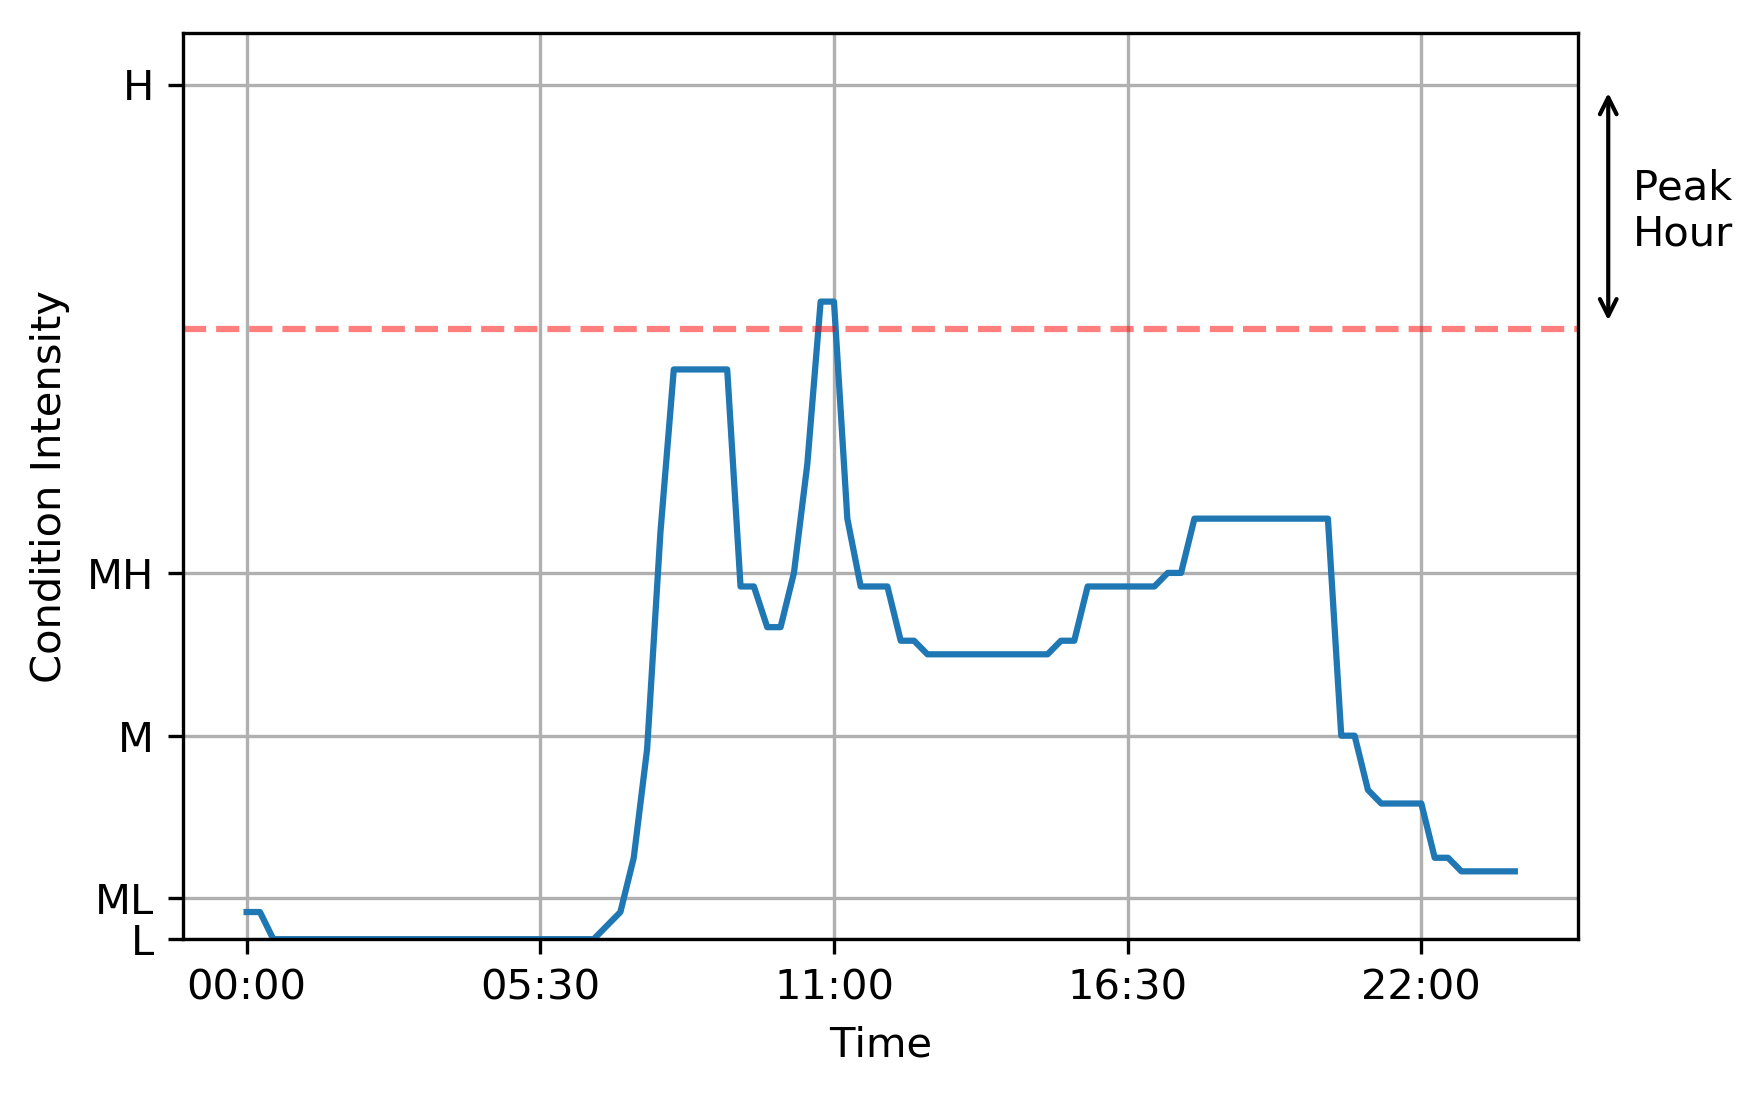
\includegraphics[width=0.5\textwidth]{figures/figure_peakhour_solution2.png}\label{figure_peakhour_solution2}}
    \caption{Examples of one-month average working day traffic of Pablo Ocampo’s southbound showing the improved peak hour detection, fixing the issues for short-term (a) below-peak hour and (b) above-peak hour condition change}

    \label{figure_peakhour_solution}
\end{figure}



Contrary to working day traffic, non-working day traffic does not have a context of peak hour. Its traffic trend only settles between near light and around moderately light due to the abundance of light traffic condition (see Figure \ref{figure_workingday_comparison}). To further support this, Figure \ref{figure_nonworkingday_peakhour} shows a visualization of the monthly average of non-working day traffic for Pablo Ocampo’s southbound and Antipolo’s northbound. Unlike working day traffic (see Table \ref{table_workingday_transition}), patterns are less recognizable due to the lack of variation of conditions for non-working day traffic (see Table \ref{table_nonworkingday_transition}).

\begin{figure}[!t] 
\centering
    \centering
      \captionsetup{justification=centering}
    \subfloat[Pablo Ocampo (Southbound)]{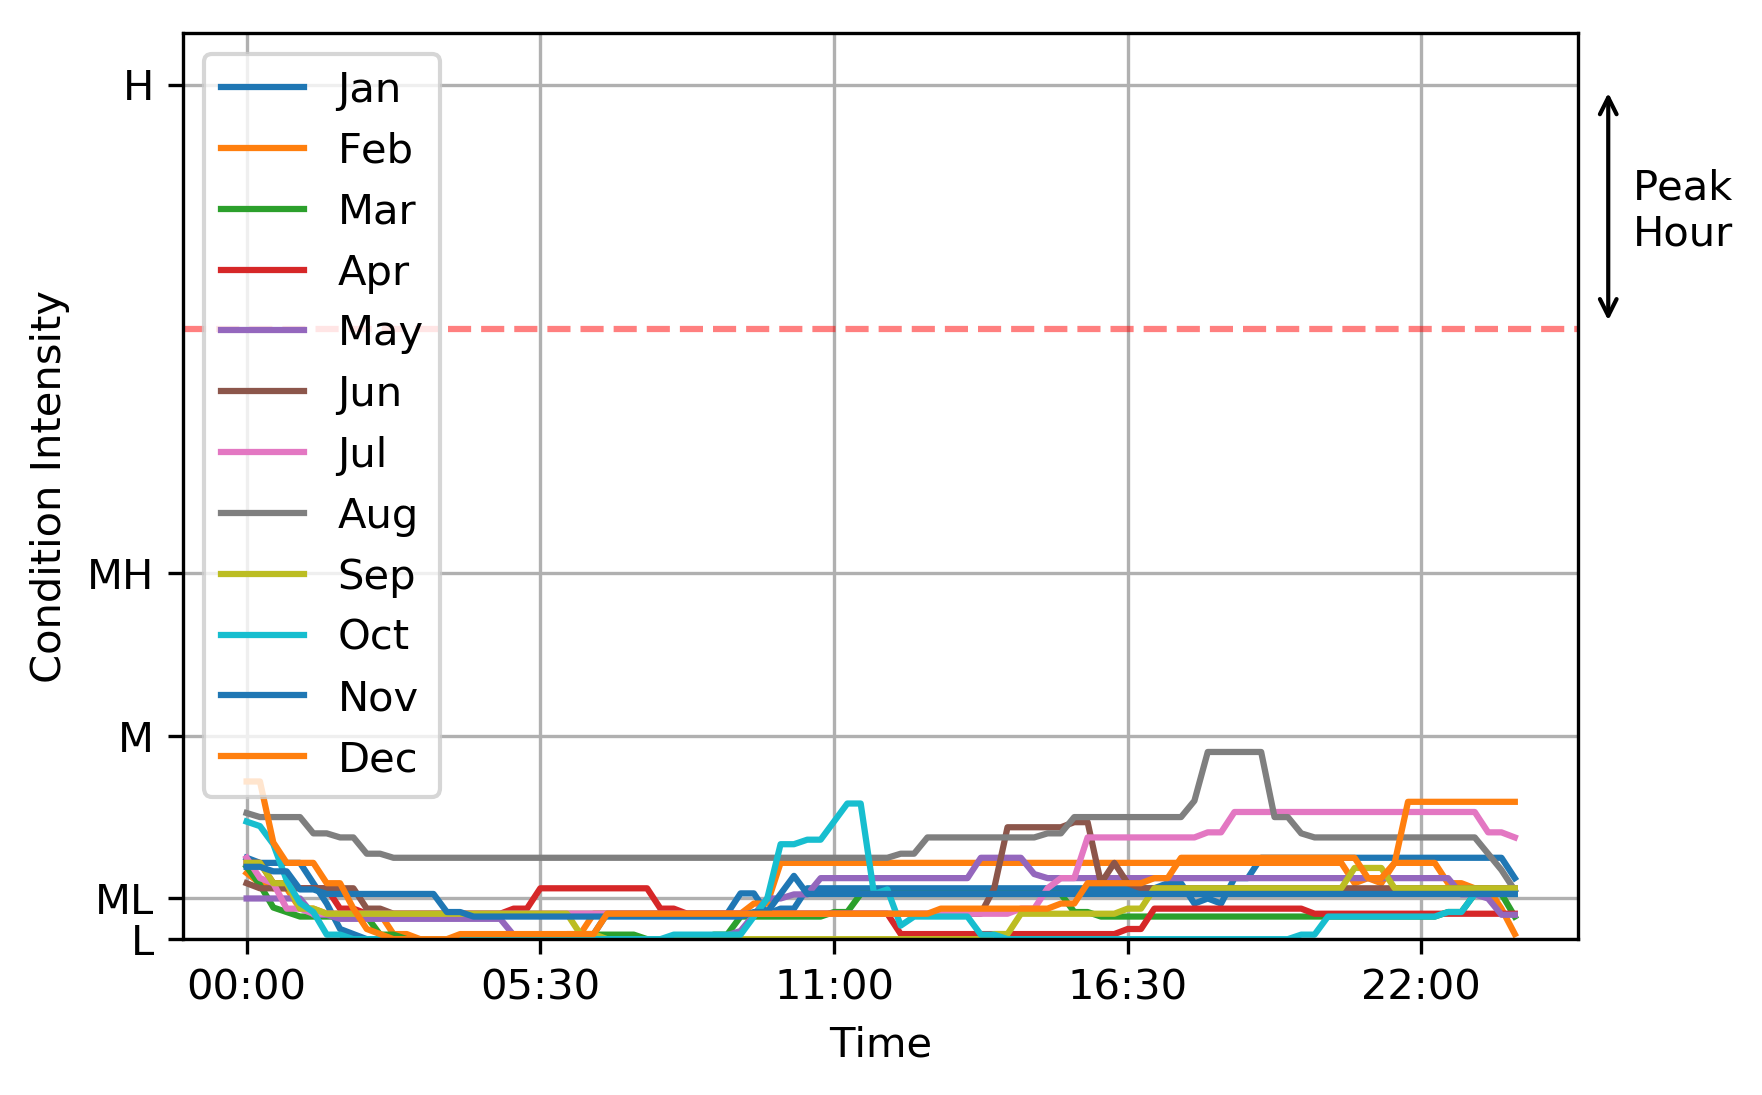
\includegraphics[width=0.5\textwidth]{figures/figure_nonworkingday_peakhour_pocampo.png}\label{figure_nonworkingday_peakhour_pocampo}}
    \hfill
    \subfloat[Antipolo (Northbound)]{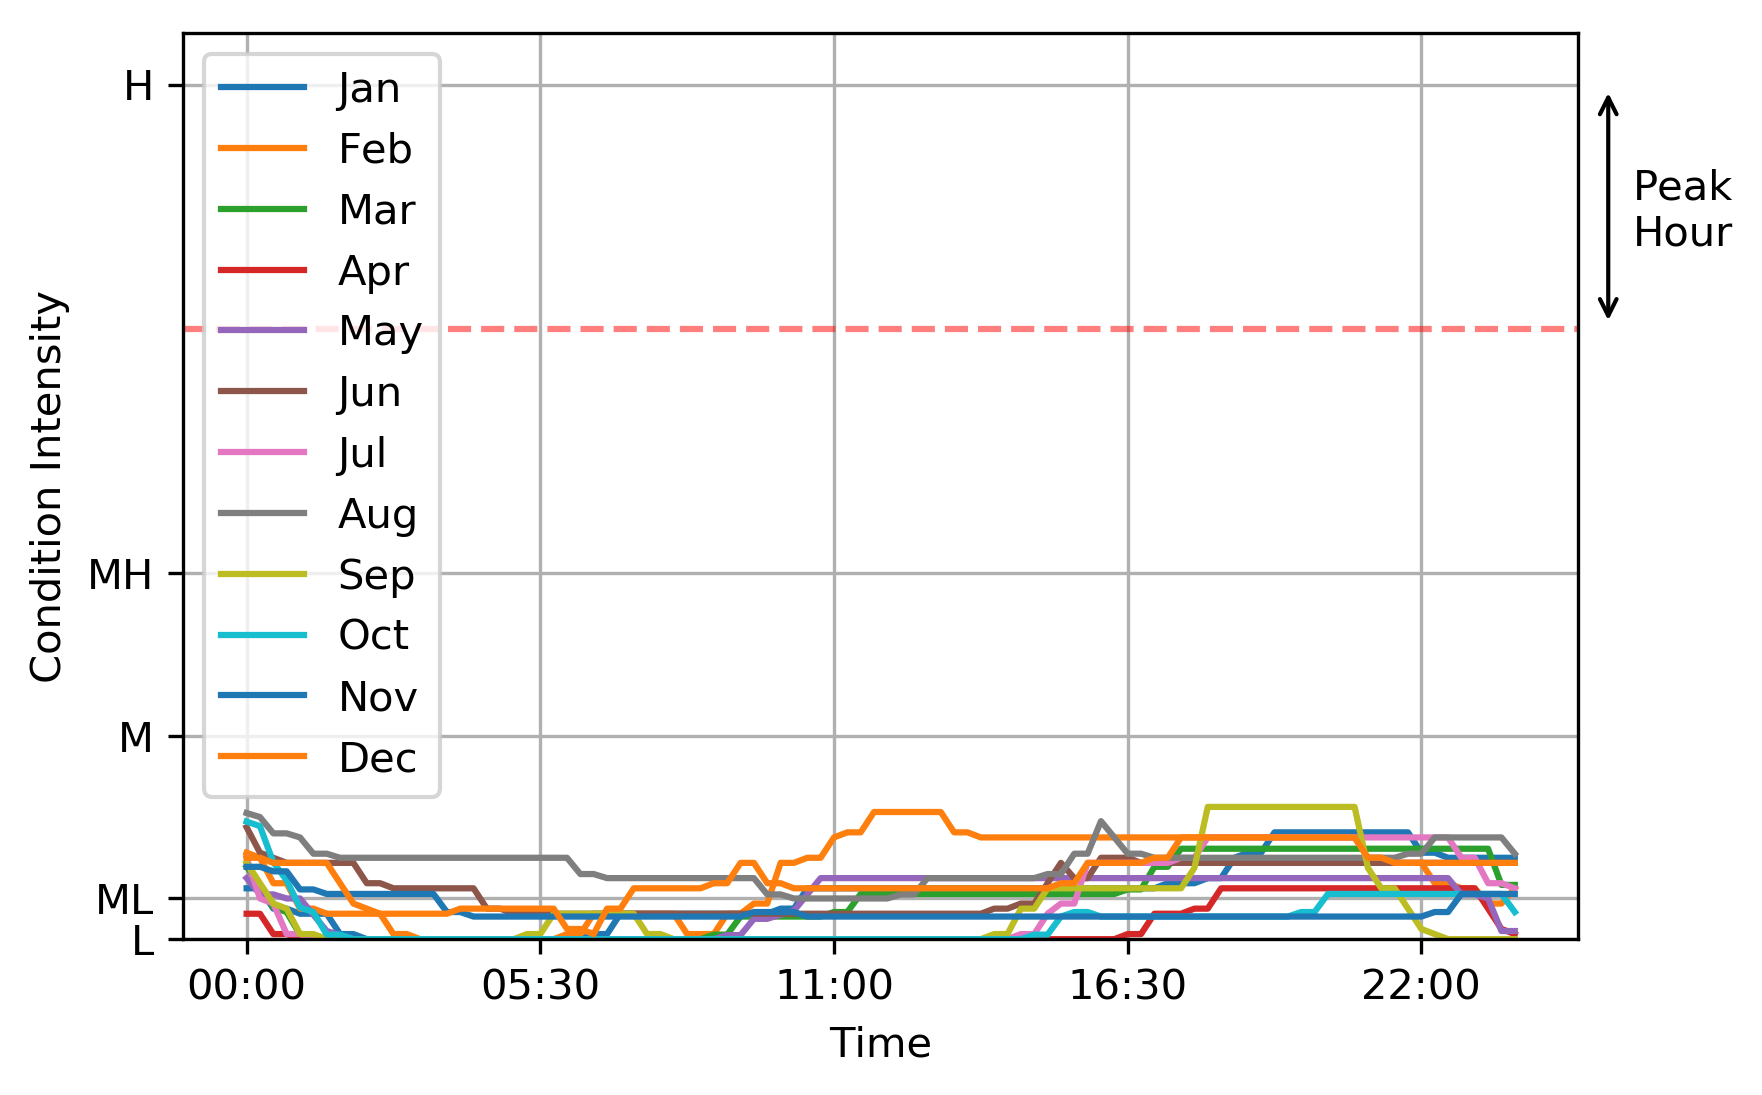
\includegraphics[width=0.5\textwidth]{figures/figure_nonworkingday_peakhour_antipolo.png}\label{figure_nonworkingday_peakhour_antipolo}}
    \caption{Monthly comparison of the average non-working day traffic of (a) Pablo Ocampo’s southbound and (b) Antipolo’s northbound }

    \label{figure_nonworkingday_peakhour}
\end{figure}
%%%%%%%%%%%%%%%%%%%%%%%%%%%%%%%
%INSERT TABLE FROM GELO

\begin{table}[!t] 
\centering
    \centering
      \captionsetup{justification=centering}
    \subfloat[ Pablo Ocampo (Southbound) distribution (\%)]{\begin{tabular}{|l|r|r|r|r|r|r|}
\hline
\multicolumn{7}{|c|}{To} \\ \hline
\multirow{6}{*}{From} & \textbf{} & L & ML & M & MH & H \\ \cline{2-7} 
 & L & 76.1 & 0.5 & 0.2 & 0.0 & 0.0 \\ \cline{2-7} 
 & ML & 0.6 & 2.1 & 0.4 & 0.0 & 0.0 \\ \cline{2-7} 
 & M & 0.0 & 0.6 & 19.0 & 0.1 & 0.0 \\ \cline{2-7} 
 & MH & 0.0 & 0.0 & 0.1 & 0.1 & 0.0 \\ \cline{2-7} 
 & H & 0.0 & 0.0 & 0.0 & 0.0 & 0.3 \\ \hline
\end{tabular}
}
    \hfill
    \subfloat[Antipolo (Northbound) distribution (\%)]{\begin{tabular}{|l|r|r|r|r|r|r|}
\hline
\multicolumn{7}{|c|}{To} \\ \hline
\multirow{6}{*}{From} & \textbf{} & L & ML & M & MH & H \\ \cline{2-7} 
 & L & 56.2 & 0.9 & 0.2 & 0.0 & 0.0 \\ \cline{2-7} 
 & ML & 1.0 & 2.3 & 0.8 & 0.0 & 0.0 \\ \cline{2-7} 
 & M & 0.0 & 1.6 & 36.4 & 0.1 & 0.0 \\ \cline{2-7} 
 & MH & 0.0 & 0.0 & 0.0 & 0.4 & 0.1 \\ \cline{2-7} 
 & H & 0.0 & 0.0 & 0.1 & 0.0 & 0.6 \\ \hline
\end{tabular}}
    \caption{Transition distribution of traffic condition of (a) Pablo Ocampo and (b) Antipolo for all non-working days}

    \label{table_nonworkingday_transition}
\end{table}



\begin{table}[!t] 
\centering
    \centering
      \captionsetup{justification=centering}
    \subfloat[ Pablo Ocampo (Southbound) distribution (\%)]{\begin{tabular}{|l|r|r|r|r|r|r|}
\hline
\multicolumn{7}{|c|}{To} \\ \hline
\multirow{6}{*}{From} & \textbf{} & L & ML & M & MH & H \\ \cline{2-7} 
 & L & 46.7 & 1.1 & 0.0 & 0.0 & 0.0 \\ \cline{2-7} 
 & ML & 1.0 & 2.2 & 1.2 & 0.0 & 0.0 \\ \cline{2-7} 
 & M & 0.1 & 1.1 & 31.9 & 0.8 & 0.0 \\ \cline{2-7} 
 & MH & 0.0 & 0.0 & 0.5 & 0.6 & 0.7 \\ \cline{2-7} 
 & H & 0.0 & 0.0 & 0.3 & 0.4 & 11.4 \\ \hline
\end{tabular}
}
    \hfill
    \subfloat[Antipolo (Northbound) distribution (\%)]{\begin{tabular}{|l|r|r|r|r|r|r|}
\hline
\multicolumn{7}{|c|}{To} \\ \hline
\multirow{6}{*}{From} & \textbf{} & L & ML & M & MH & H \\ \cline{2-7} 
 & L & 29.5 & 1.1 & 0.0 & 0.0 & 0.0 \\ \cline{2-7} 
 & ML & 1.0 & 2.2 & 1.1 & 0.0 & 0.0 \\ \cline{2-7} 
 & M & 0.1 & 1.0 & 41.0 & 0.6 & 0.0 \\ \cline{2-7} 
 & MH & 0.0 & 0.0 & 0.6 & 0.5 & 0.6 \\ \cline{2-7} 
 & H & 0.0 & 0.0 & 0.1 & 0.5 & 20.1 \\ \hline
\end{tabular}}
    \caption{Transition distribution of traffic condition of (a) Pablo Ocampo and (b) Antipolo for all working days}

    \label{table_workingday_transition}
\end{table}

%%%%%%%%%%%%%%%%%%%%%%%%%%%%%%%


\subsubsection{Week Before}
In Figure \ref{figure_traffic_day_vs_week}, it could be observed how closer the traffic pattern is with its week before pattern compared with its two-days-ago pattern. Referring at the identified traffic seasonality in Figure \ref{figure_autocorr_week}, we could see how an observation in traffic appears to be more seasonal with its previous weeks as compared with the preceding days, with exception to the day before a specific observation.

\begin{figure}[!t] 
\centering
    \centering
      \captionsetup{justification=centering}
    \subfloat[Pablo Ocampo (Southbound)]{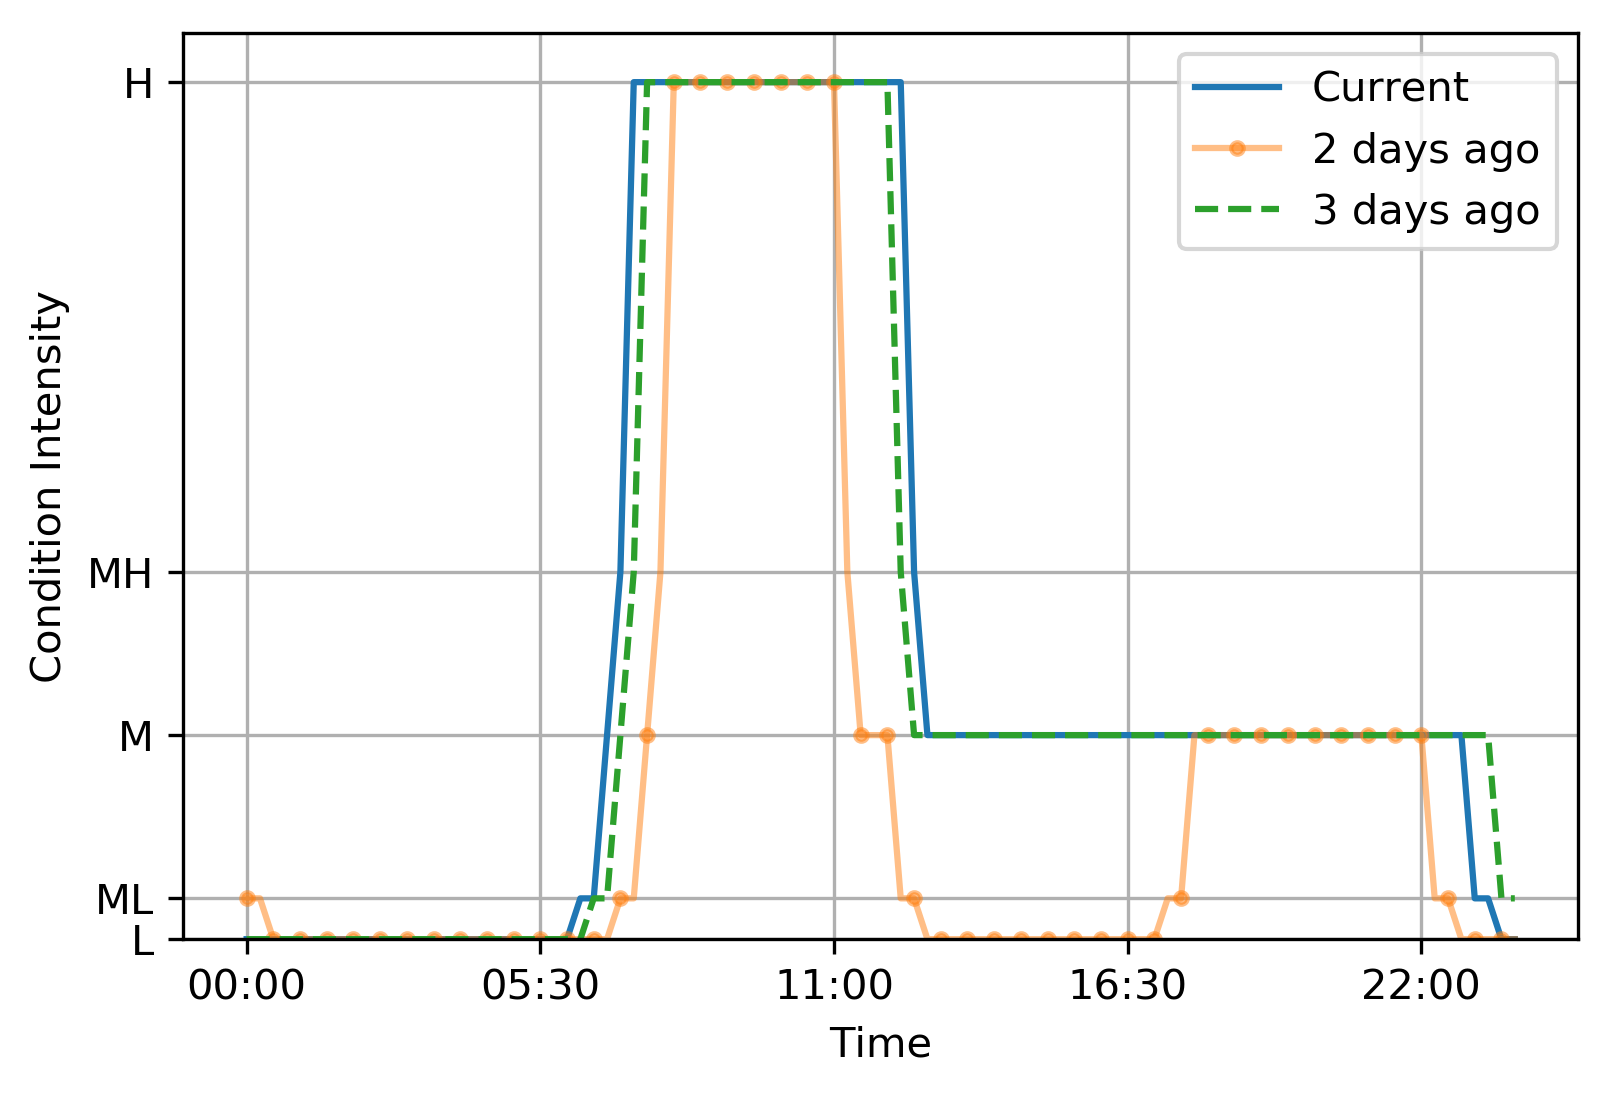
\includegraphics[width=0.5\textwidth]{figures/figure_traffic_day_vs_week_pocampo.png}\label{figure_traffic_day_vs_week_pocampo}}
    \hfill
    \subfloat[Antipolo (Northbound)]{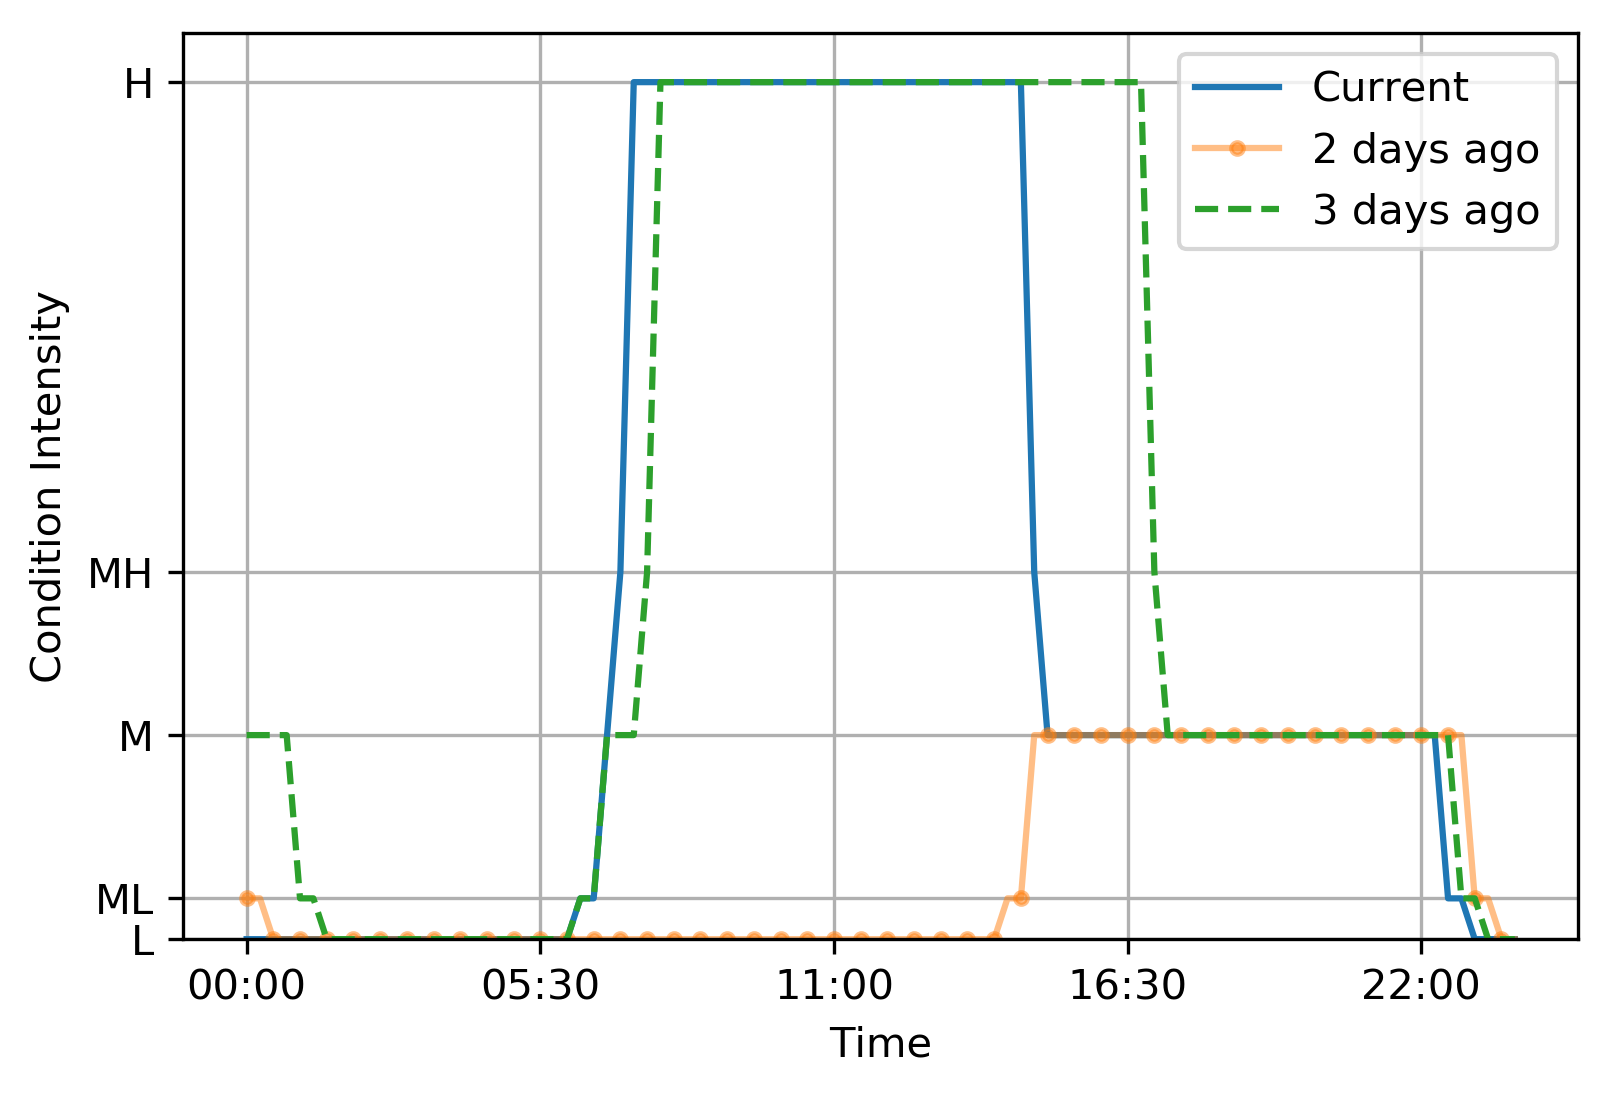
\includegraphics[width=0.5\textwidth]{figures/figure_traffic_day_vs_week_antipolo.png}\label{figure_traffic_day_vs_week_antipolo}}
    \caption{Comparison between the two-day-ago pattern and one-week-ago pattern of (a) Pablo Ocampo’s southbound and (b) Antipolo’s northbound traffic pattern showing that the week before traffic is more similar despite its difference in terms of days}

    \label{figure_traffic_day_vs_week}
\end{figure}



%%%%%%%%%%%%%%%%%%%%%%%%%%%%%%%%%%%%%%%%%%%%%%%%%%%%
%insert more analysis
%%%%%%%%%%%%%%%%%%%%%%%%%%%%%%%%%%%%%%%%%%%%%%%%%%%%

\subsection{Weather Analysis}

Performing Spearman's rank correlation on weather variables against traffic, in general, reveals that they have a weak correlation (see Figure \ref{figure_corr_trafficweather}). One possible reason for this is the effects of weather to traffic is not immediate. For instance, changes in traffic pattern are not immediately seen upon the start of precipitation. Instead, it can be seen after a while as precipitation continues building up. To address this problem, an exploratory analysis between each weather variables and traffic are conducted, exploring their commonalities in terms of seasonality and trends.


\begin{figure}[!t]
  \centering
  \captionsetup{justification=centering}
  \scalebox{0.5}{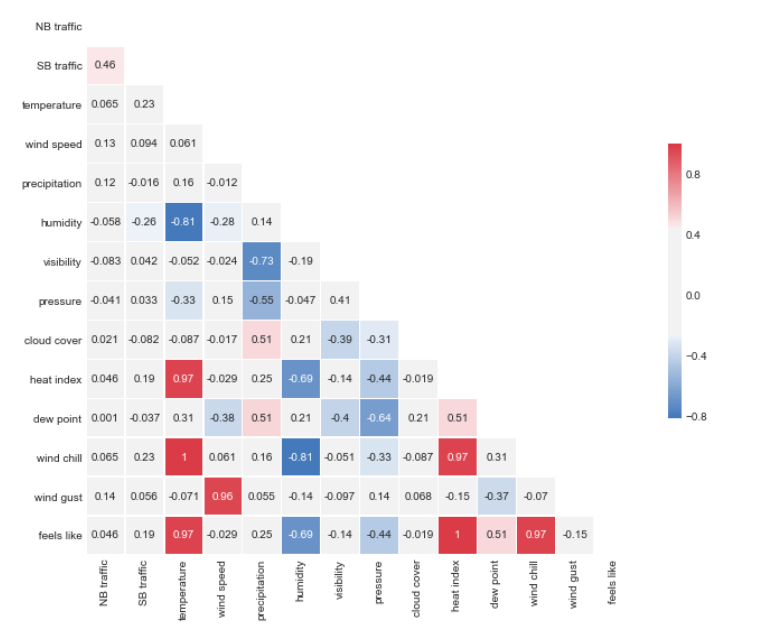
\includegraphics{figure_corr_trafficweather.PNG}}
  \caption{Correlation heatmap of traffic (Pablo Ocampo and Antipolo) and weather variables showing a weak correlation between them}
\label{figure_corr_trafficweather}
\end{figure}



\subsubsection{Seasonality}

Similar to traffic, the autocorrelation of each weather variable reveals that all of them have a daily seasonality (see Figure \ref{figure_autocorr_weather}). Notably, the majority of them are able to maintain their seasonality for days or even a week. Nevertheless, these are not true for weather variables such as precipitation, visibility, wind speed, and wind gust, which are seasonal to their previous day yet have a weak relationship with it.


\begin{figure}[!t]
  \centering
  \captionsetup{justification=centering}
  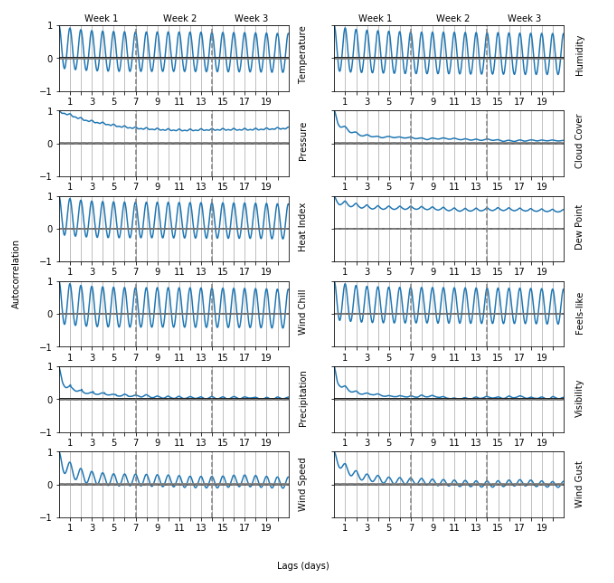
\includegraphics[width=1.0\textwidth]{figure_autocorr_weather.PNG}
  \caption{Autocorrelation of weather variables showing the presence of daily seasonality}
\label{figure_autocorr_weather}
\end{figure}

%Autocorrelation of weather variables showing the presence of daily seasonality
%\label{figure_autocorr_weather}

\subsubsection{Trend}

As traffic is able to maintain a relatively moderate seasonality with its previous days, weather variables whose seasonalities are characterized similarly will be explored. These will include temperature, pressure, heat index, wind chill, humidity, dew point, and feels-like. To define their normal trend, their daily average per time intervals will be utilized, given by its daily seasonality. In consideration for the case of traffic, however, priority will be given to the SB traffic as it has a relatively stronger relationship with other weather variables as compared with NB traffic, and only working days on a given month will be considered with respect to its previous day seasonality.

\paragraph{Temperature, Heat Index, Feels-Like and Wind Chill}

Figure \ref{figure_traffic_vs_tempheatfeelswind} illustrates a one-month visualization of the normal trend of temperature, heat index, feels-like and wind chill against traffic. From the initial correlation analysis mentioned earlier (see Figure \ref{figure_corr_trafficweather}), temperature, heat index, feels-like and wind chill has a weak correlation of 0.2 and 0.3 with Pablo Ocampo’s southbound and Antipolo’s northbound traffic respectively. A reason for this is despite that they match in terms of their morning trend, their evening trend significantly differs. Moreover, interpreting this relationship, it only shows the transition of dawn to morning, or simply the beginning of the morning peak hour.


\begin{figure}[!t] 
\centering
    \centering
      \captionsetup{justification=centering}
    \subfloat[Pablo Ocampo (Southbound)]{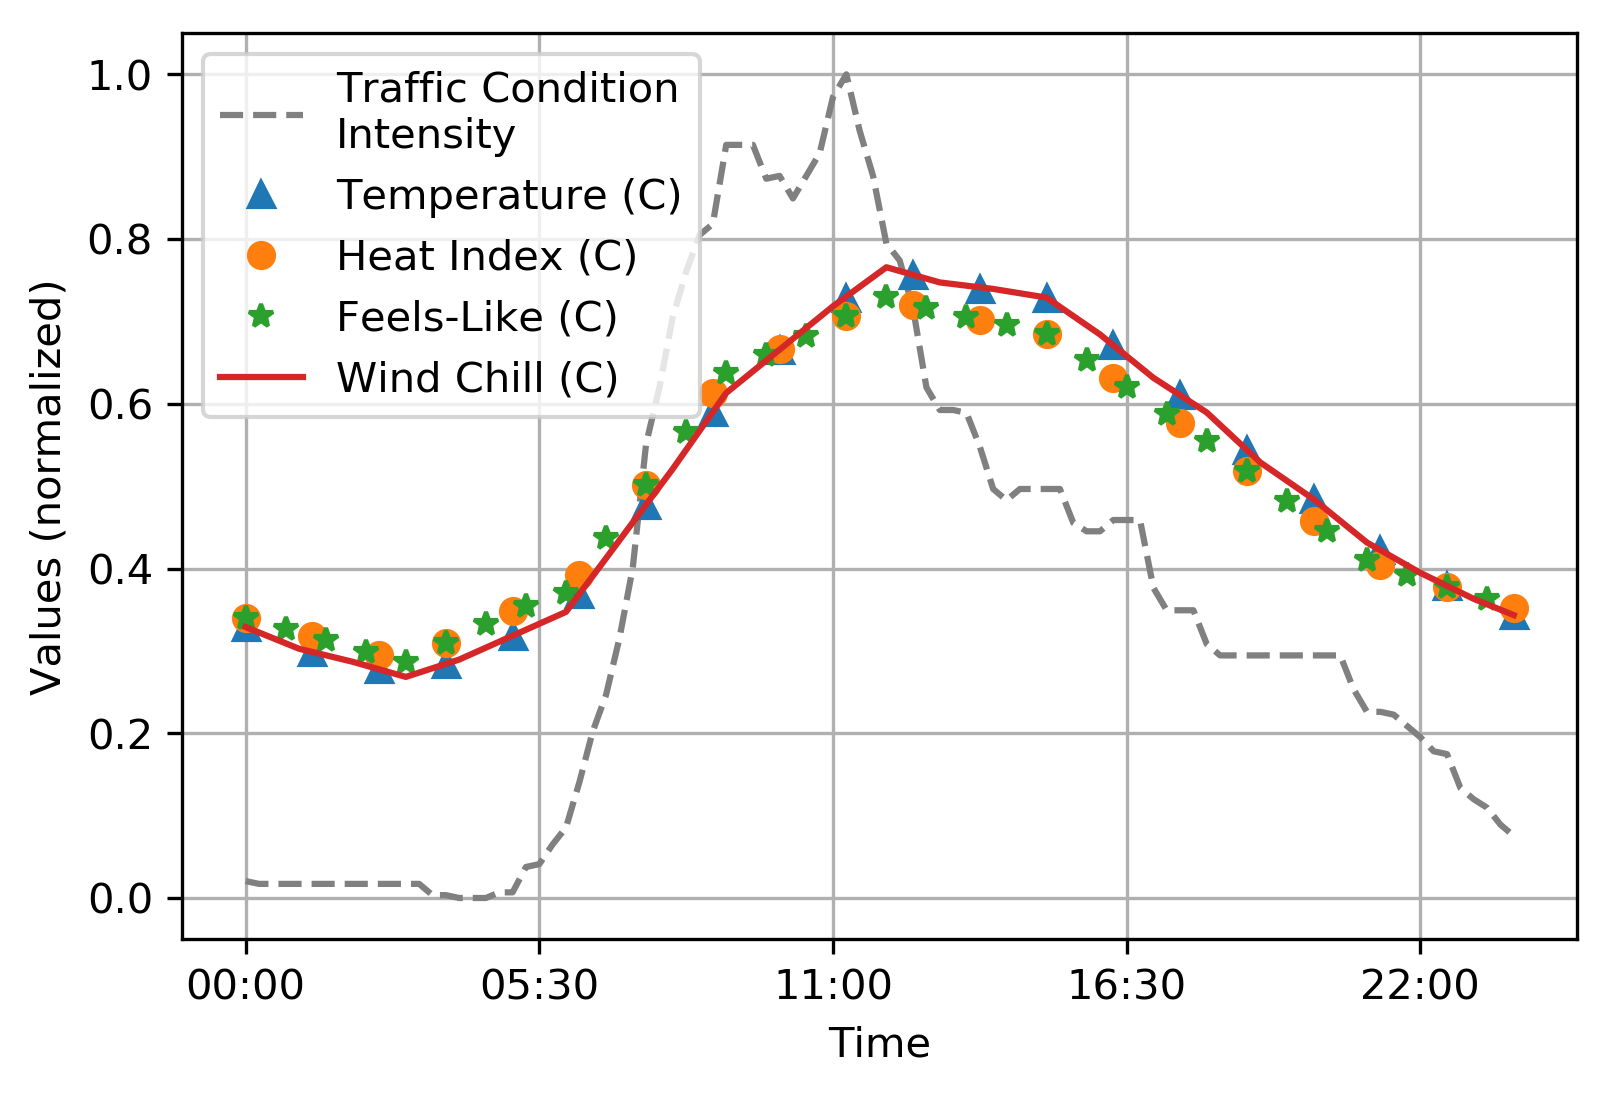
\includegraphics[width=0.5\textwidth]{figures/figure_traffic_vs_tempheatfeelswind_pocampo.png}\label{figure_traffic_vs_tempheatfeelswind_pocampo}}
    \hfill
    \subfloat[Antipolo (Northbound)]{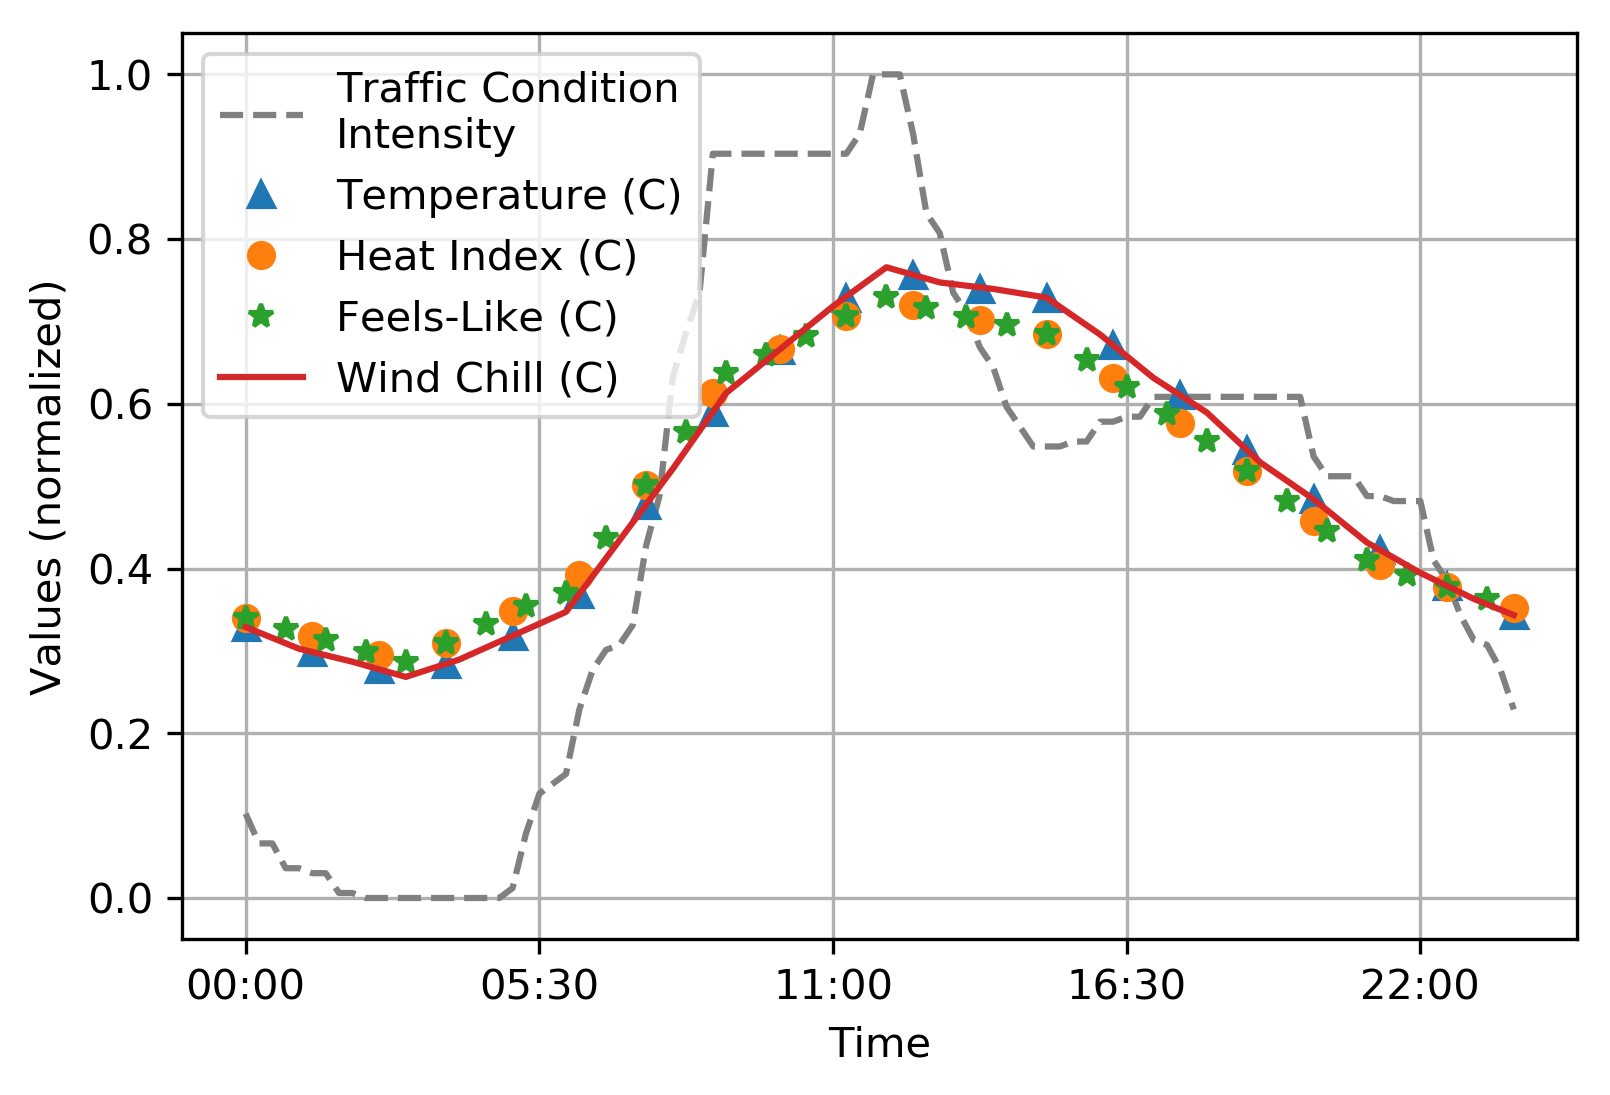
\includegraphics[width=0.5\textwidth]{figures/figure_traffic_vs_tempheatfeelswind_antipolo.png}\label{figure_traffic_vs_tempheatfeelswind_antipolo}}
    \caption{Comparison of the normal pattern of temperature, heat index, feels-like and wind chill with the normal pattern of Pablo Ocampo’s southbound and Antipolo’s northbound traffic}

    \label{figure_traffic_vs_tempheatfeelswind}
\end{figure}


%Comparison of the normal pattern of temperature, heat index, feels-like and wind chill with the normal pattern of traffic
%\label{figure_traffic_vs_tempheatfeelswind}
%%%%%%%%%%%%%%%%%%%%%%%%%%%%%%%%%%%%%%%%%%%%%%%%%%%%%55
\paragraph{Pressure}

Figure \ref{figure_traffic_vs_pressure} shows a one-month visualization of the normal trend of pressure and traffic. At initial glance, it resembles the traffic pattern in a subtle way. However, looking at the initial correlation analysis earlier (see Figure \ref{figure_corr_trafficweather}), pressure appeared to have a significantly weak correlation with traffic, at 0.033. One notable difference between pressure and traffic is that pressure rises again during the evening up to dawn, following its relationship with temperature \shortcite{aguado2007understanding}.


\begin{figure}[!t] 
\centering
    \centering
      \captionsetup{justification=centering}
    \subfloat[Pablo Ocampo (Southbound)]{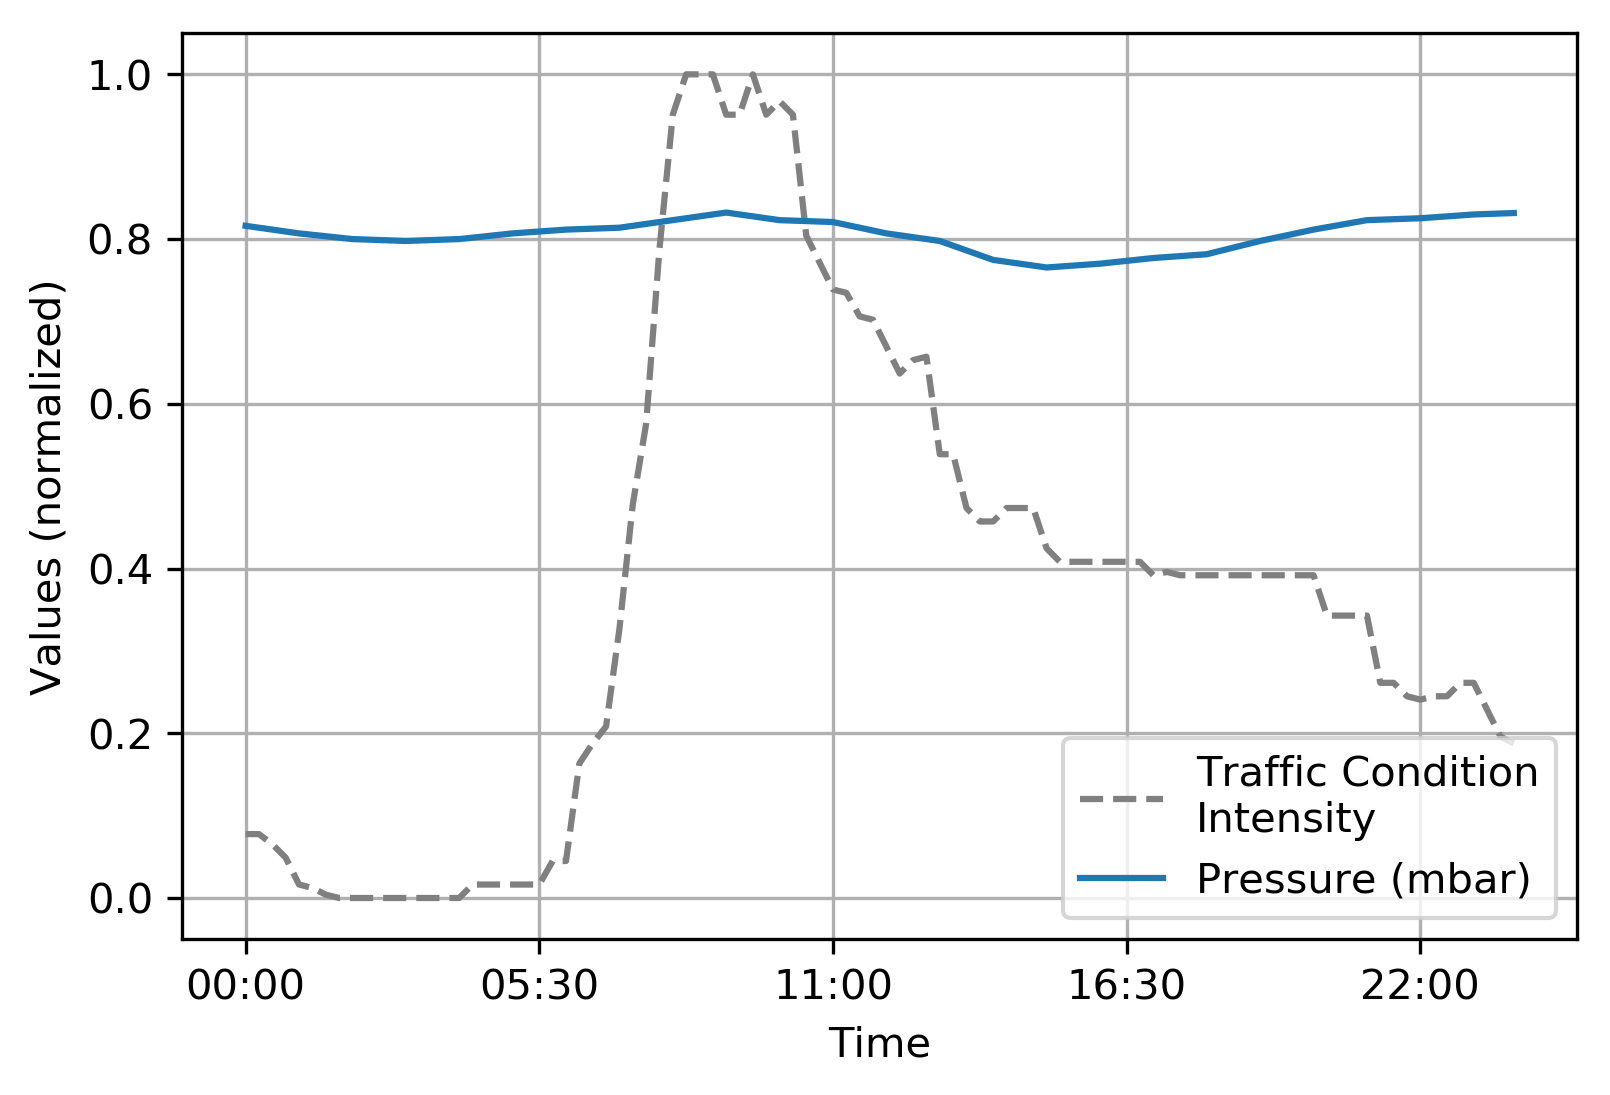
\includegraphics[width=0.5\textwidth]{figures/figure_traffic_vs_pressure_pocampo.png}\label{figure_traffic_vs_pressure_pocampo}}
    \hfill
    \subfloat[Antipolo (Northbound)]{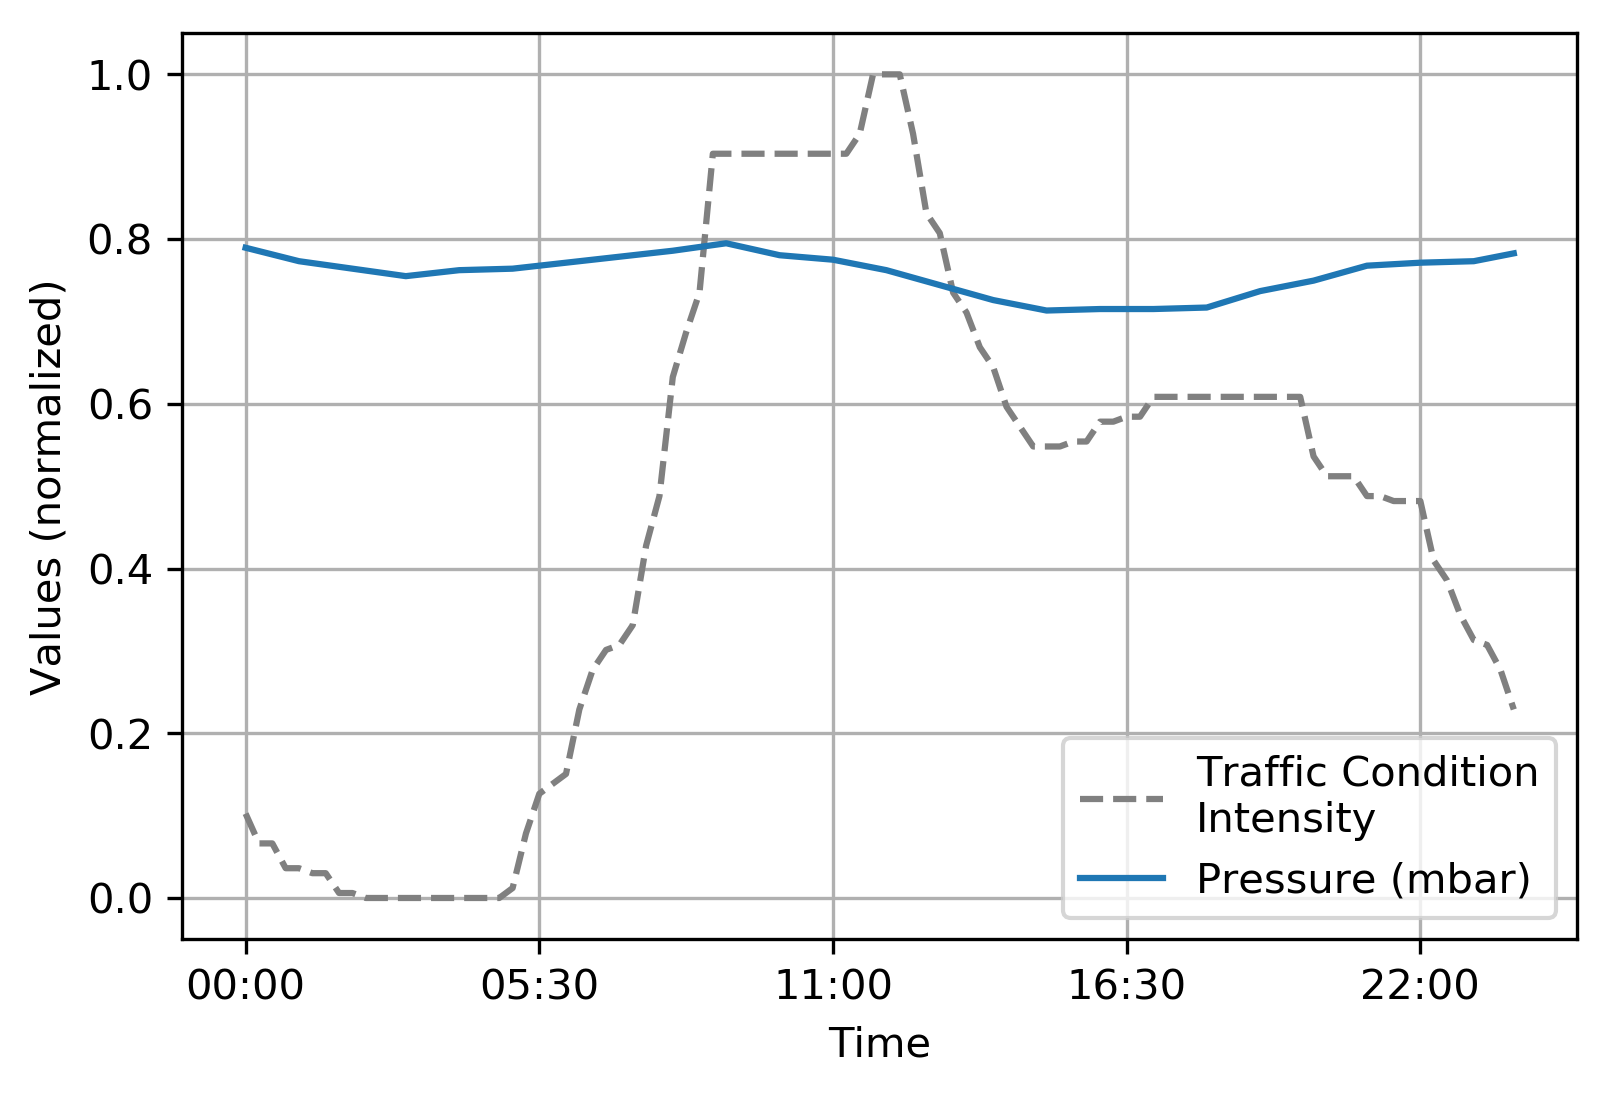
\includegraphics[width=0.5\textwidth]{figures/figure_traffic_vs_pressure_antipolo.png}\label{figure_traffic_vs_pressure_antipolo}}
    \caption{Comparison of the normal pattern of pressure with the normal pattern of Pablo Ocampo’s southbound and Antipolo’s northbound traffic}

    \label{figure_traffic_vs_pressure}
\end{figure}


%Comparison of the normal pattern of pressure with the normal pattern of traffic
%\label{figure_traffic_vs_pressure}

\paragraph{Humidity}

Figure \ref{figure_traffic_vs_humidity} illustrates a one-month visualization of the normal trend of humidity and traffic. Basing on the initial correlation (see Figure \ref{figure_corr_trafficweather}), humidity has a weak correlation of -0.260 with traffic. Comparatively, this could be interpreted in the same way as temperature yet reversed due to its negative relationship, following the relationship of temperature and humidity \shortcite{paull1999effect}. This is further supported by the strong negative relationship between temperature and humidity with a value of -0.810.

\begin{figure}[!t] 
\centering
    \centering
      \captionsetup{justification=centering}
    \subfloat[Pablo Ocampo (Southbound)]{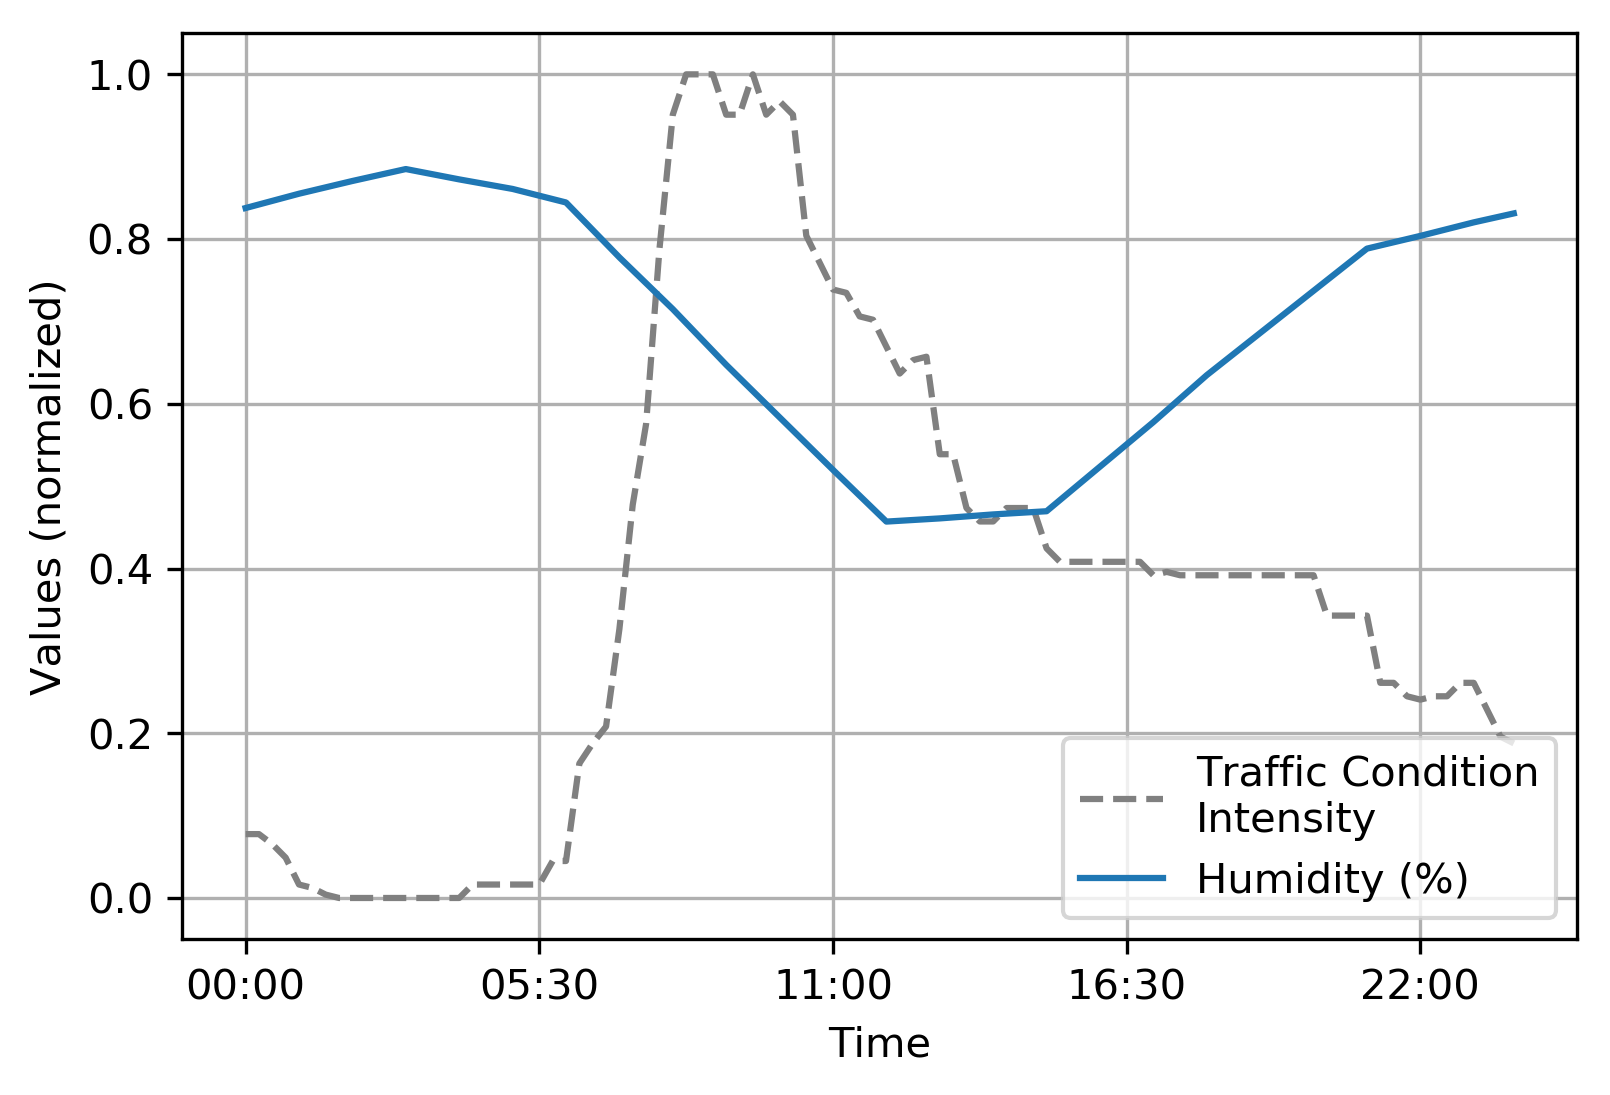
\includegraphics[width=0.5\textwidth]{figures/figure_traffic_vs_humidity_pocampo.png}\label{figure_traffic_vs_humidity_pocampo}}
    \hfill
    \subfloat[Antipolo (Northbound)]{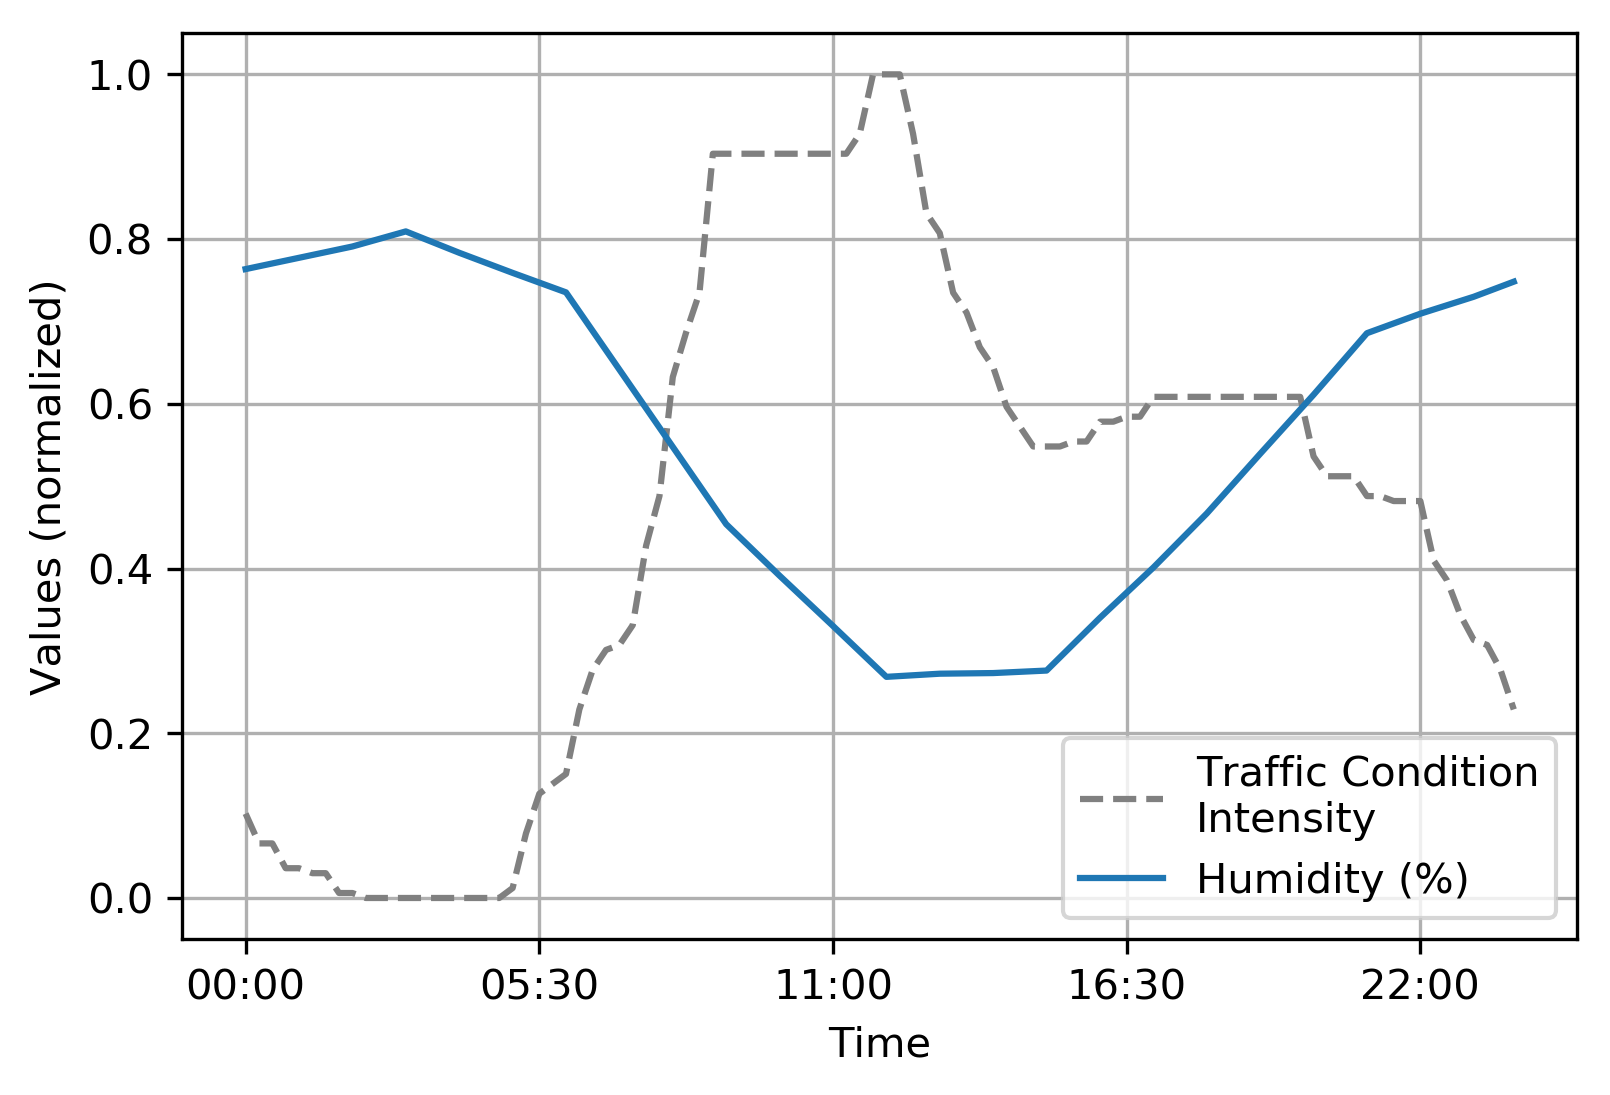
\includegraphics[width=0.5\textwidth]{figures/figure_traffic_vs_humidity_antipolo.png}\label{figure_traffic_vs_humidity_antipolo}}
    \caption{Comparison of the normal pattern of humidity with the normal pattern of Pablo Ocampo’s southbound and Antipolo’s northbound traffic}

    \label{figure_traffic_vs_humidity}
\end{figure}

% Comparison of the normal pattern of humidity with the normal pattern of traffic
% \label{figure_traffic_vs_humidity}

\paragraph{Dew Point}

Figure \ref{figure_traffic_vs_dewpoint} shows a one-month visualization of the normal trend of dew point and traffic. Upon initial inspection, there is a subtle similarity between its pattern with the pattern of traffic. However, referring to the initial correlation (see Figure \ref{figure_corr_trafficweather}), dew point has a significantly weak correlation of -0.037 with traffic. Rather, this similarity in terms of form may be due to its relationship with pressure \shortcite{gaul1952relation}.

\begin{figure}[!t] 
\centering
    \centering
      \captionsetup{justification=centering}
    \subfloat[Pablo Ocampo (Southbound)]{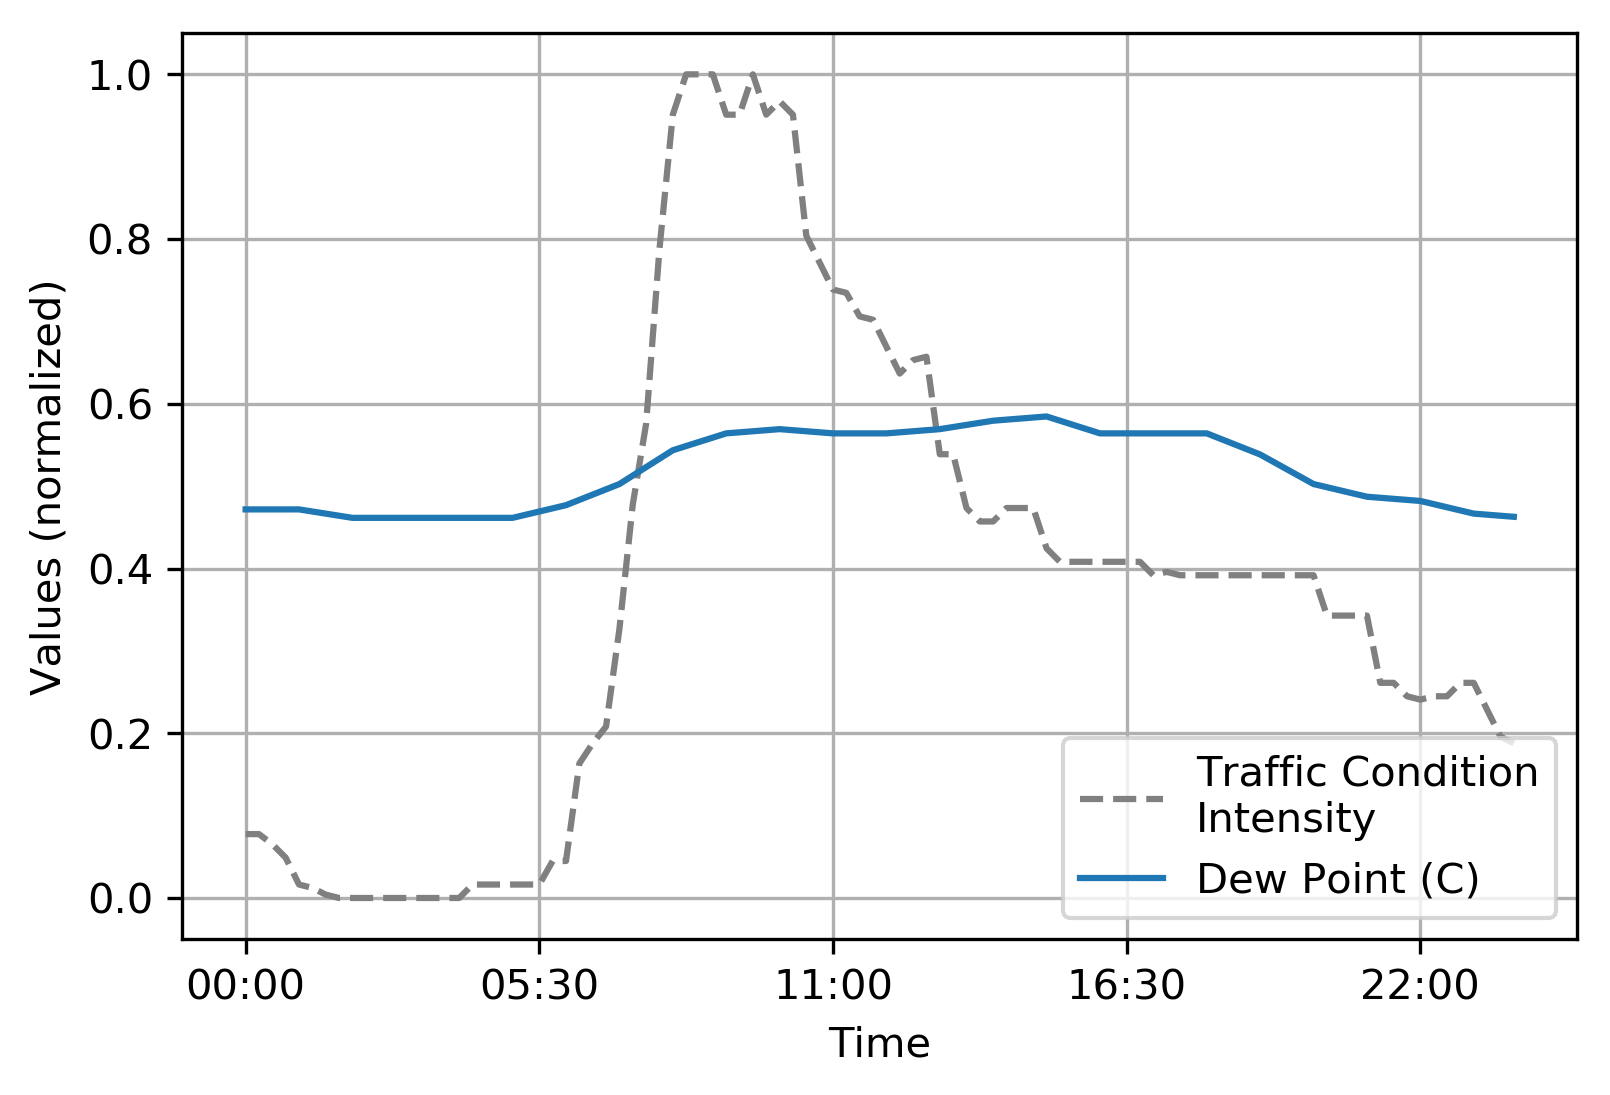
\includegraphics[width=0.5\textwidth]{figures/figure_traffic_vs_dewpoint_pocampo.png}\label{figure_traffic_vs_dewpoint_pocampo}}
    \hfill
    \subfloat[Antipolo (Northbound)]{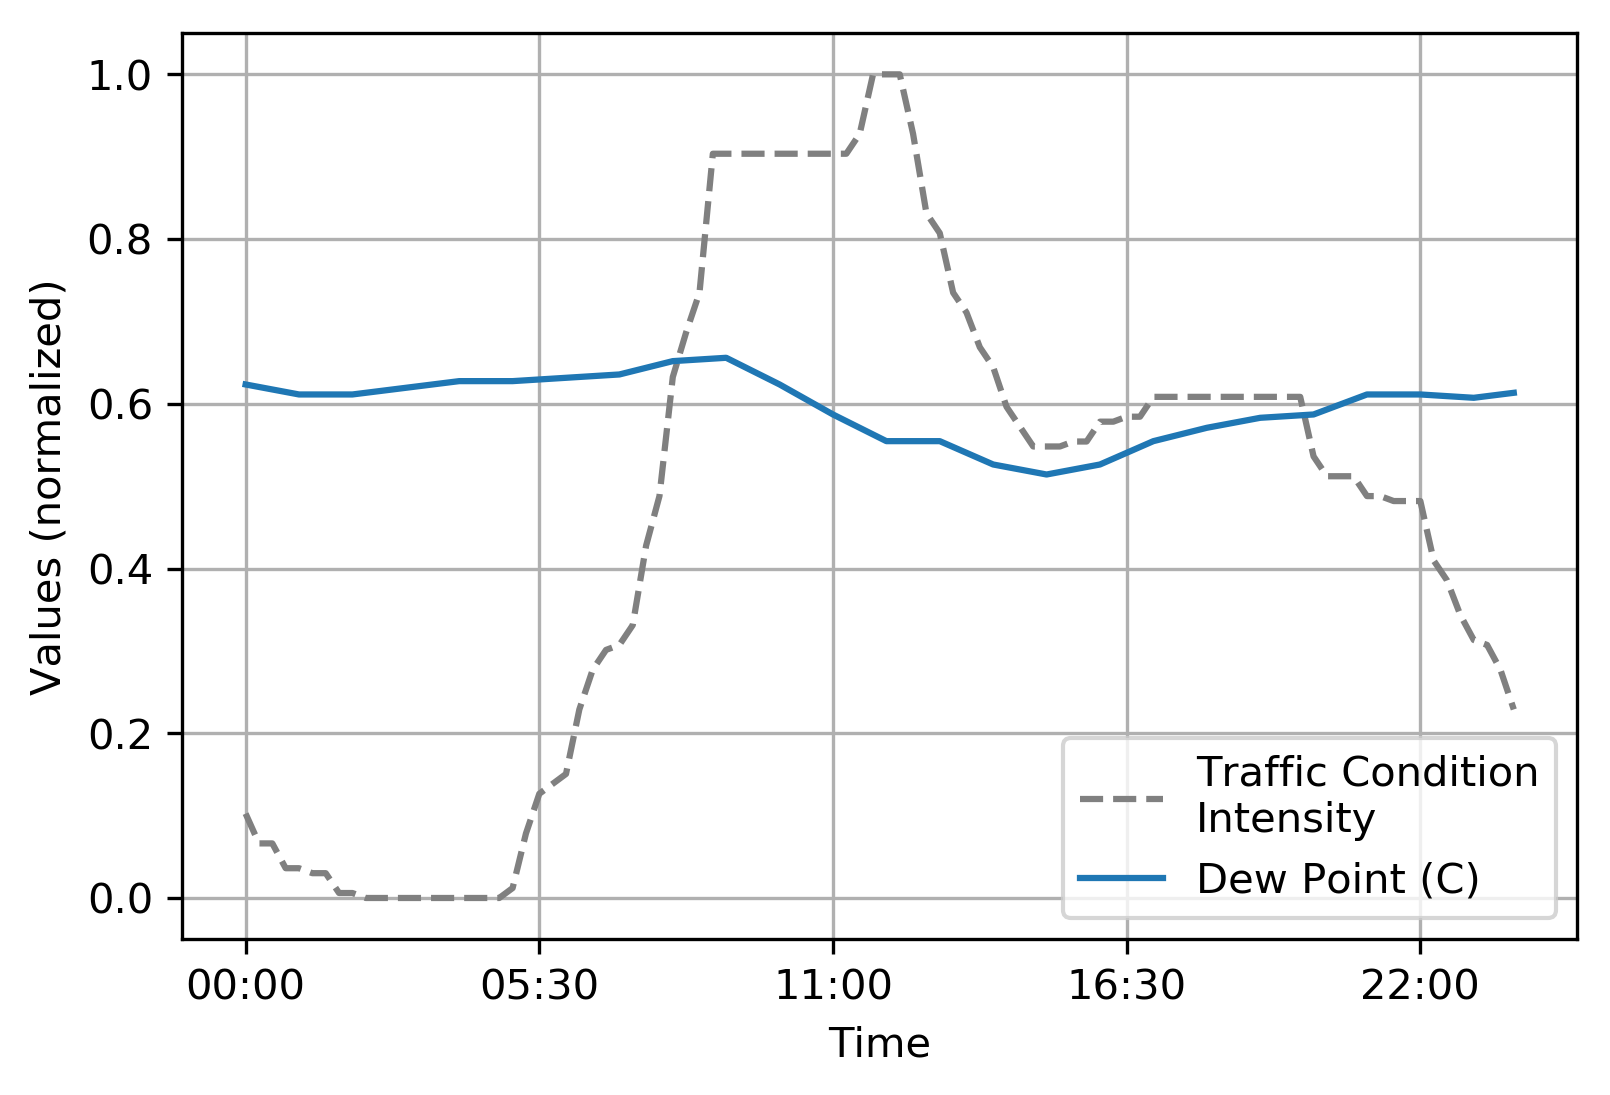
\includegraphics[width=0.5\textwidth]{figures/figure_traffic_vs_dewpoint_antipolo.png}\label{figure_traffic_vs_dewpoint_antipolo}}
    \caption{Comparison of the normal pattern of dew point with the normal pattern of Pablo Ocampo’s southbound and Antipolo’s northbound traffic}

    \label{figure_traffic_vs_dewpoint}
\end{figure}


In summary, based on exploratory analysis, there is no derivable relationship between weather variables and traffic. This might be due to the fact that contributing factors to traffic are already embedded in its respective conditions, or traffic, itself, has its own pattern to follow. As the examined variables gradually change, as characterized by their consistently strong week-long seasonality, there is no abrupt or noticeable impact in terms of the daily traffic pattern.

\subsection{Weather Disruption}
As there was no established relationship between weather variables and normal traffic pattern, another way to analyze the relationship of weather to traffic is by exploring its special cases, particularly when there are extreme weather conditions such as typhoons and low-pressure areas that may disrupt the usual pattern of traffic. To assess this, the criteria for classifying a weather-disrupted day are identified.

\subsubsection{Climate Season}

According to \shortciteA{pagasa_climate}, dry and wet season occurs from December to May and June to November respectively. However, contrary to this, the precipitation data from 2015-2017 shows that the dry season occurs from January to April, and wet season strongly occurs from May to October (see Figure \ref{figure_ave_precip}).

\begin{figure}[!t]
  \centering
  \captionsetup{justification=centering}
  \scalebox{.65}{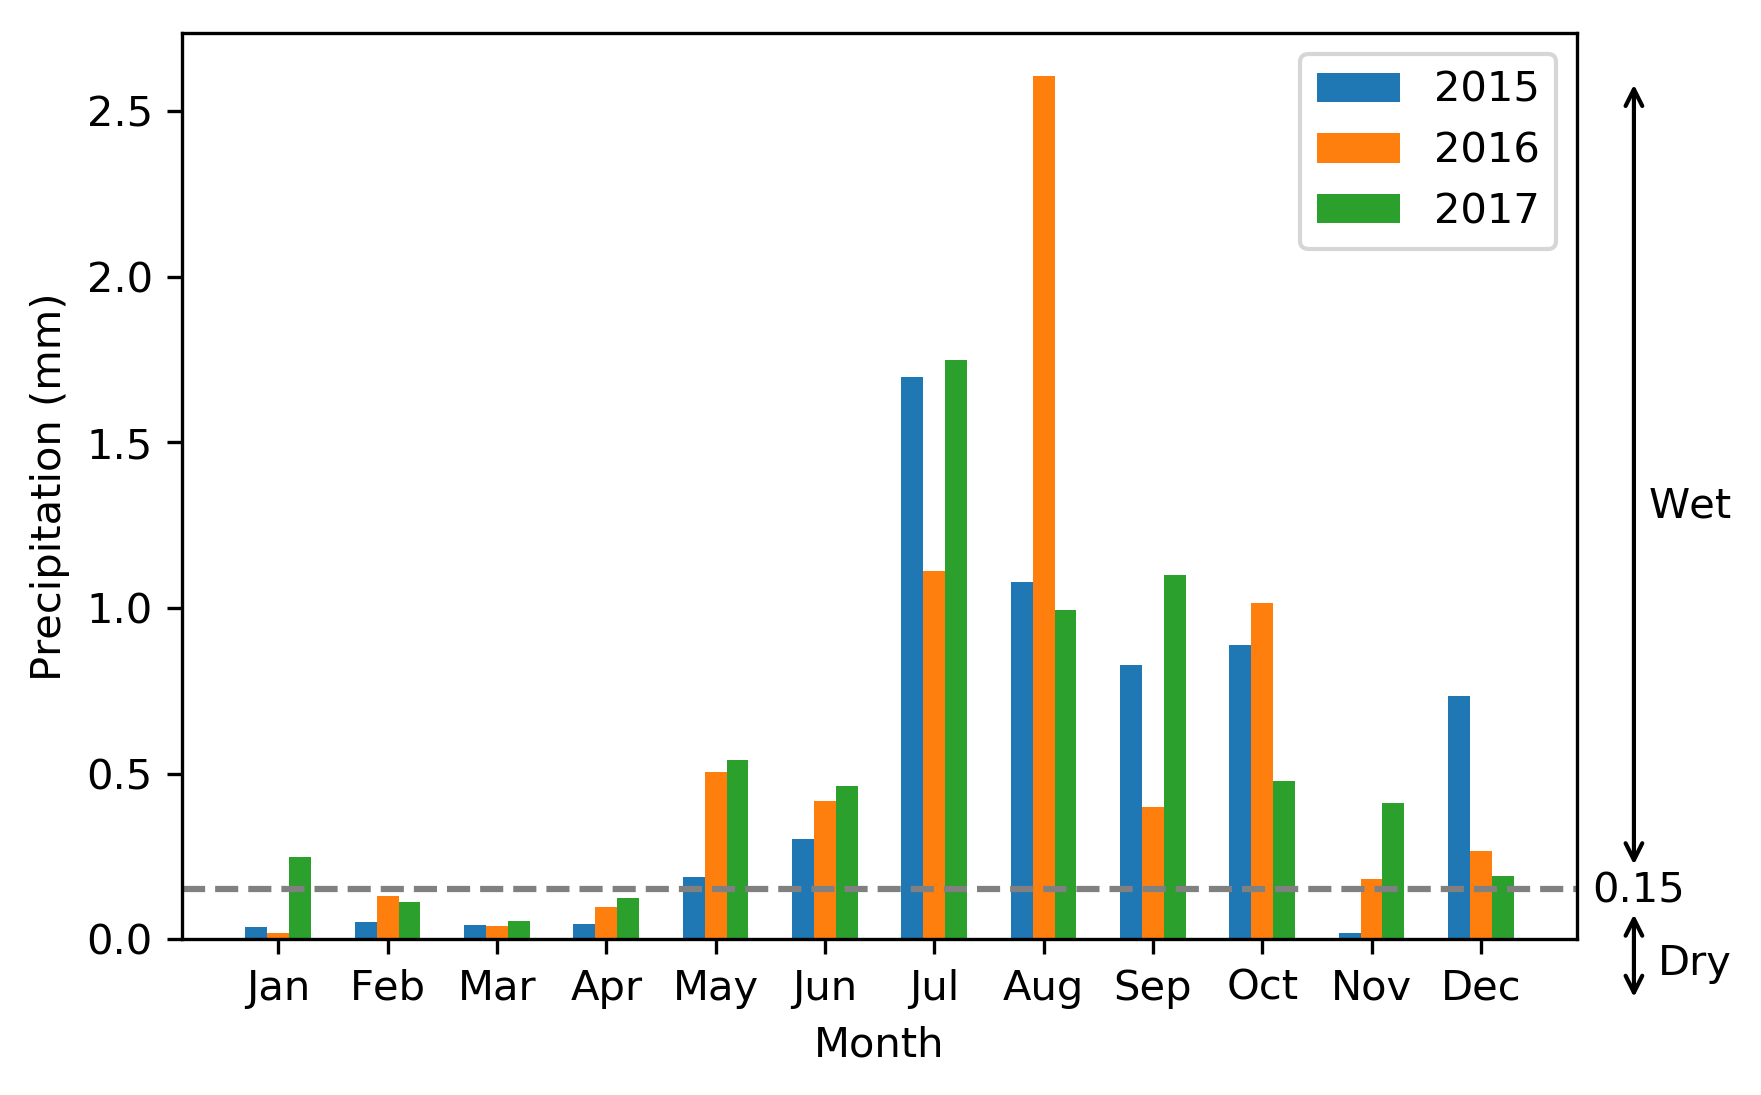
\includegraphics{figures/figure_ave_precip.PNG}}
  \caption{Wet and dry season based on the average precipitation per month from 2015 to 2017 defined by the 0.15mm threshold}
\label{figure_ave_precip}
\end{figure}

% Wet and dry season defined by the average precipitation per month from 2015 to 2017
% \label{figure_ave_precip}


\subsubsection{Disrupted Day}

IIt is important to note that when defining disrupted days in respect to traffic, there are two factors to consider. First, it has been established by analyzing the traffic trends that increase in traffic mostly occur around 6:00. Thus, to observe the effects of prolonged rainfall to traffic, the instances of precipitation during the evening should be disregarded as its effect is more likely to decay when it is expected to effect during the morning. In the following experiments, only weather instances from 0:00 to 21:00 will be observed.

Second, only working days are considered as these are the days when traffic is significantly dynamic, hence disruption on its pattern can be observed. Given this, similar in our previous experiments in traffic, holidays and suspensions are considered as outliers as its traffic pattern would be inconsistent with its usual working day pattern.

Meanwhile, for weather, a threshold should be made with respect to the number of intervals per day. Given that a day is defined by 96 15-minute intervals, a cumulative minimum of 28 intervals or 7 hours of rain condition will be set as the threshold in classifying a disrupted day.

With these criteria set, a total of 69 disrupted days have been identified, in which 44.92\% came from working days under the typhoon. As expected, the majority of these are taken from the wet season, more specifically 94.20\% of it.


\subsection{Traffic Disruption}
Comparing the autocorrelation between dry and wet season, it could be observed that the daily seasonality of traffic becomes less evident during the wet season (see Figure \ref{figure_autocorr_traffic_season}). This could be due to the abundance of precipitation, disrupting the normal pattern of traffic.


\begin{figure}[!t] 
\centering
    \centering
      \captionsetup{justification=centering}
    \subfloat[Dry Season]{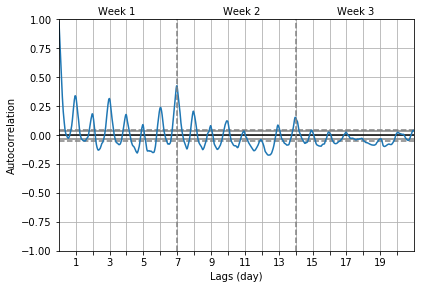
\includegraphics[width=0.5\textwidth]{figures/figure_traffic_autocorr_dryseason.png}\label{figure_traffic_autocorr_dryseason}}
    \hfill
    \subfloat[Wet Season]{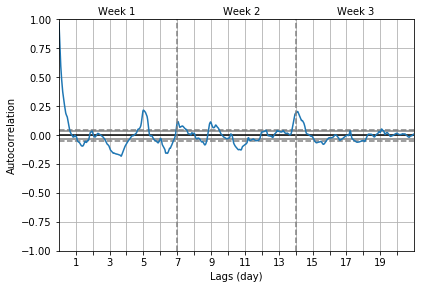
\includegraphics[width=0.5\textwidth]{figures/figure_traffic_autocorr_wetseason.png}\label{figure_traffic_autocorr_wetseason}}
    \caption{Autocorrelation of traffic comparing the daily and weekly seasonality per season showing that its pattern is disrupted during the wet season}
    \label{figure_autocorr_traffic_season}
\end{figure}

% Dry Season
% \label{figure_traffic_autocorr_dryseason}

% (b) Wet Season
% \label{figure_traffic_autocorr_wetseason}

% Autocorrelation of traffic comparing the daily and weekly seasonality per season showing that its pattern is disrupted during the wet season
% \label{figure_autocorr_traffic_season}

To verify this, we compare one observation of traffic (a week before Typhoon Goring) with its previous week (on the week of the typhoon). Basing from the seasonality of traffic, it is expected that the current traffic pattern would be similar to its previous week (see Figure \ref{figure_traffic_disrupted}). However, visualizing the current traffic pattern with its previous week, it could be observed that there is a significant increase in traffic as compared with the previous week of traffic.

\begin{figure}[!t] 
\centering
  \scalebox{.85}{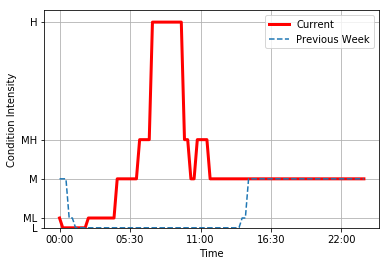
\includegraphics{figures/figure_traffic_disrupted.png}}
  \caption{Comparison between the current traffic and its previous week pattern showing a disrupted pattern}
  \label{figure_traffic_disrupted}
\end{figure}

% Comparison between the current traffic and its previous week pattern showing a disrupted pattern
% \label{figure_traffic_disrupted}








\section{Correlation Analysis}
\subsection{Correlation of Engineered Traffic Features with Traffic Condition}

\subsubsection{Mean of Previous Weeks}
As the weekly seasonality of traffic remains consistent in both dry and wet season, the previous weeks could be potentially used to override the disrupted pattern of the previous week of a specific observation. In identifying this pattern, the mean of the traffic for the past weeks are taken. Correlating against the previous day and previous week seasonality, we could immediately observe an increase in the strength of its relationship with the present traffic (see Table \ref{table_corr_nomean_vs_mean}).


\begin{table}[]
\centering
\caption{Comparison between previous day and week traffic with the traffic mean 4-weeks-ago showing significant increase in strength in its relationship}
\label{table_corr_nomean_vs_mean}
\begin{tabular}{|l|r|}
\hline
                                                                            & \textbf{Correlation value} \\ \hline
\textbf{\begin{tabular}[c]{@{}l@{}}Previous Day\\ Traffic\end{tabular}}     & 0.265                      \\ \hline
\textbf{\begin{tabular}[c]{@{}l@{}}Previous Week\\ Traffic\end{tabular}}    & 0.282                      \\ \hline
\textbf{\begin{tabular}[c]{@{}l@{}}Traffic Mean\\ 4-weeks-ago\end{tabular}} & 0.391                      \\ \hline
\end{tabular}
\end{table}

% Comparison between previous day and week traffic with the traffic mean 4-weeks-ago showing significant increase in strength in its relationship
% \label{table_corr_nomean_vs_mean}

Further experimenting with the strength of its relationship, we examined the correlation of from 2-weeks-ago traffic up to 7-days-ago traffic (see Table \ref{table_corr_mean}). From this, we have identified the ideal range to be 6 weeks ago, as the relationship already starts to fade when 7 weeks ago is reached. Interestingly, the traffic mean 2-weeks-ago has a weaker relationship to the current traffic than the succeeding number of weeks. This could be due to the fact that at 2 weeks, there exist only the traffic of the previous week and the traffic 2 weeks ago. Considering the observation at the previous week is disrupted, then the effect of it is not minimized as you’re only aggregating it against one more value.



\begin{table}[]
\centering
\caption{Comparison of correlation values on the traffic mean of a range of weeks}
\label{table_corr_mean}
\begin{tabular}{|l|r|}
\hline
\textbf{\begin{tabular}[c]{@{}l@{}}Traffic Mean\\ N-weeks-ago\end{tabular}} & \textbf{Correlation value} \\ \hline
\textbf{2}                                                                  & 0.293                      \\ \hline
\textbf{3}                                                                  & 0.327                      \\ \hline
\textbf{4}                                                                  & 0.391                      \\ \hline
\textbf{5}                                                                  & 0.399                      \\ \hline
\textbf{6}                                                                  & \textbf{0.418}             \\ \hline
\textbf{7}                                                                  & 0.411                      \\ \hline
\textbf{8}                                                                  & 0.405                      \\ \hline
\end{tabular}
\end{table}


% Comparison of correlation values on the traffic mean of a range of weeks
% \label{table_corr_mean}

To verify this finding, Figure \ref{figure_traffic_mean_2weeks_vs_6weeks} illustrates an observation from an undisrupted time span, comparing the similarity of the current pattern with the traffic mean 6 weeks ago and 2 weeks ago. From this, it could be observed how close the current pattern with the mean of the traffic 6 weeks ago, specifically from 6:00 to 13:00.


\begin{figure}[!t] 
\centering
  \scalebox{.90}{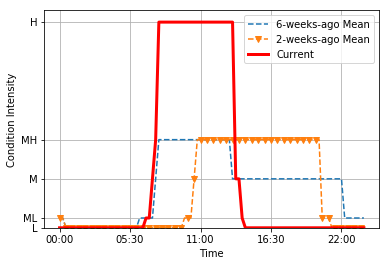
\includegraphics{figures/figure_traffic_mean_2weeks_vs_6weeks.png}}
  \caption{One-day visualization of the relationship between the current traffic and the mean of the traffic 6 weeks ago and 2 weeks ago}
  \label{figure_traffic_mean_2weeks_vs_6weeks}
\end{figure}


% One-day visualization of the relationship between the current traffic and the mean of the traffic 6 weeks ago and 2 weeks ago
% \label{figure_traffic_mean_2weeks_vs_6weeks}

This observation holds true even in disrupted days. Figure \ref{figure_traffic_mean_2weeks_vs_6weeks_disrupted} shows an observation after a week of Typhoon Goring. It could be seen in this visualization that the 6-weeks-ago traffic mean appeared to be more similar to the pattern of the current traffic as compared with the 2-weeks-ago traffic mean. As mentioned earlier, this could be due to the fact that getting the mean of just two observations where one is disrupted may not be enough to capture the undisrupted relationship of the previous weeks of traffic.

\begin{figure}[!t] 
\centering
  \centering
  \scalebox{.85}{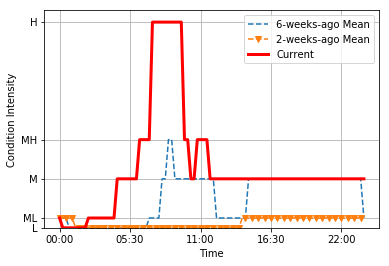
\includegraphics{figures/figure_traffic_mean_2weeks_vs_6weeks_disrupted.png}}
  \caption{One-day visualization of the relationship between the current traffic and the mean of the traffic 6 weeks ago and 2 weeks ago after a week of Typhoon Goring}
  \label{figure_traffic_mean_2weeks_vs_6weeks_disrupted}
\end{figure}


% One-day visualization of the relationship between the current traffic and the mean of the traffic 6 weeks ago and 2 weeks ago after a week of Typhoon Goring
% \label{figure_traffic_mean_2weeks_vs_6weeks_disrupted}

\subsubsection{Rolling and Expanding Features}

The data only describes the traffic condition per timestep and the seasonality of traffic. Although traffic has pattern, there are instances when a certain disruption in traffic may cause congestion build up. Therefore, considering how the immediate past traffic conditions may affect the current traffic condition can be considered as a factor for predicting traffic. Data  from the previous timestep can be used as a reference in predicting the current traffic condition. However, the change in traffic in a 15-minute timeframe may not be significant. As seen in Figure \ref{autocorr_whyRE}, autocorrelation reveals that a traffic condition is highly likely to reoccur every 15 minutes. In other words, the traffic condition of the previous time step is highly likely to be the traffic condition of the current time step. However, this does not capture the effects of sudden outliers to the build up or decay of traffic. Thus, it does not fully describe how the past traffic conditions might affect the current traffic condition. 


\begin{figure}[!t] 
\centering
  \centering
  \scalebox{.4}{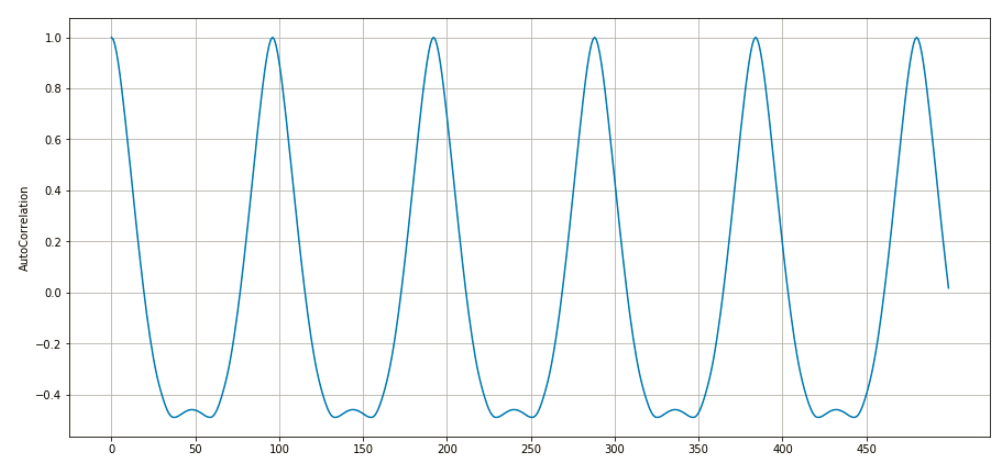
\includegraphics{figures/autocorr_whyRE.PNG}}
  \caption{Autocorrelation of traffic for working days}
  \label{autocorr_whyRE}
\end{figure}

% Autocorrelation of traffic for working days
% \label{autocorr_whyRE}

Generating rolling and expanding features based on a specific window size gives a bigger look as to what the current traffic might be based from the previous traffic conditions. Rolling and expanding window traffic features such as the mean, the minimum, and the maximum with window size  4, 8, 24, 48, and 96 were generated from the original traffic data. To summarize the possible effects of sudden changes in traffic, the mean of the past traffic conditions based on a window size was generated. Figure \ref{stDev} shows the standard deviation values of traffic for every window size. Standard deviation shows the variability or the distance of the data from the mean. From this, it can be observed that there is a rising pattern in the growth of the standard deviation as the window size increases. The low standard deviation of smaller window sizes signifies that there is only a little to no change in traffic condition within that time frame. Meanwhile, large window sizes like window 96 which yield a relatively larger standard deviation value of 0.03531 than of window 4, implies that the traffic conditions in a 1-day time frame are more varied or are more widely spread. With small window sizes, the values generated captures less of the trifle changes in traffic and gets more affected by outlier values which then results in a more generic information. However, as the window size increases, the effect of outlier values also get more neutralized because of the number of data considered, giving a broader summary of the past traffic. 

\begin{figure}[!t] 
\centering
  \centering
  \scalebox{.85}{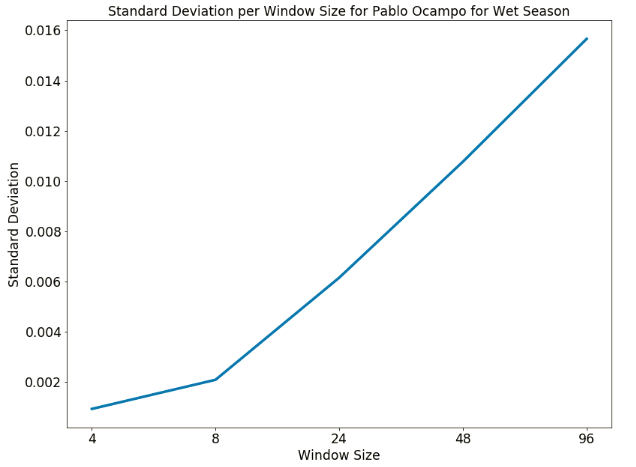
\includegraphics{figures/pocampo_stdev.PNG}}
  \caption{Standard Deviation of Traffic per Window Size for the Wet Season in Pablo Ocampo}
  \label{stDev}
\end{figure}

% Standard Deviation of Traffic per Window Size for the Wet Season in Antipolo
% \label{stDev}

The minimum and maximum features, on the other hand, reveals the range of x in the dataset. Being sensitive to outliers, they provide outlier detection when compared to the average value of that specific set of data. A big difference between the values of the minimum and the maximum signifies a large progression in traffic condition. Although as the window size used gets bigger, it becomes harder to determine whether the sudden change in traffic condition occurred just a few timesteps before or if it is because of a farther instance which may have less to no effect to the current traffic condition. 

\begin{figure}[t] 
\centering
    \centering
      \captionsetup{justification=centering}
    \subfloat[Original vs. Rolling]{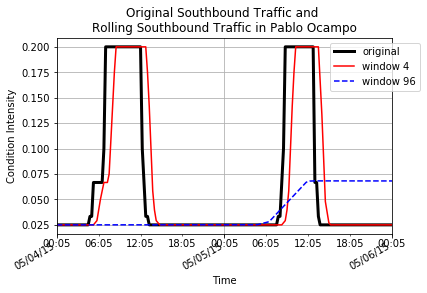
\includegraphics[width=0.5\textwidth]{figures/pocampo_rolling.png}\label{pocampo_rolling}}
    \hfill
    \subfloat[Original vs. Expanding]{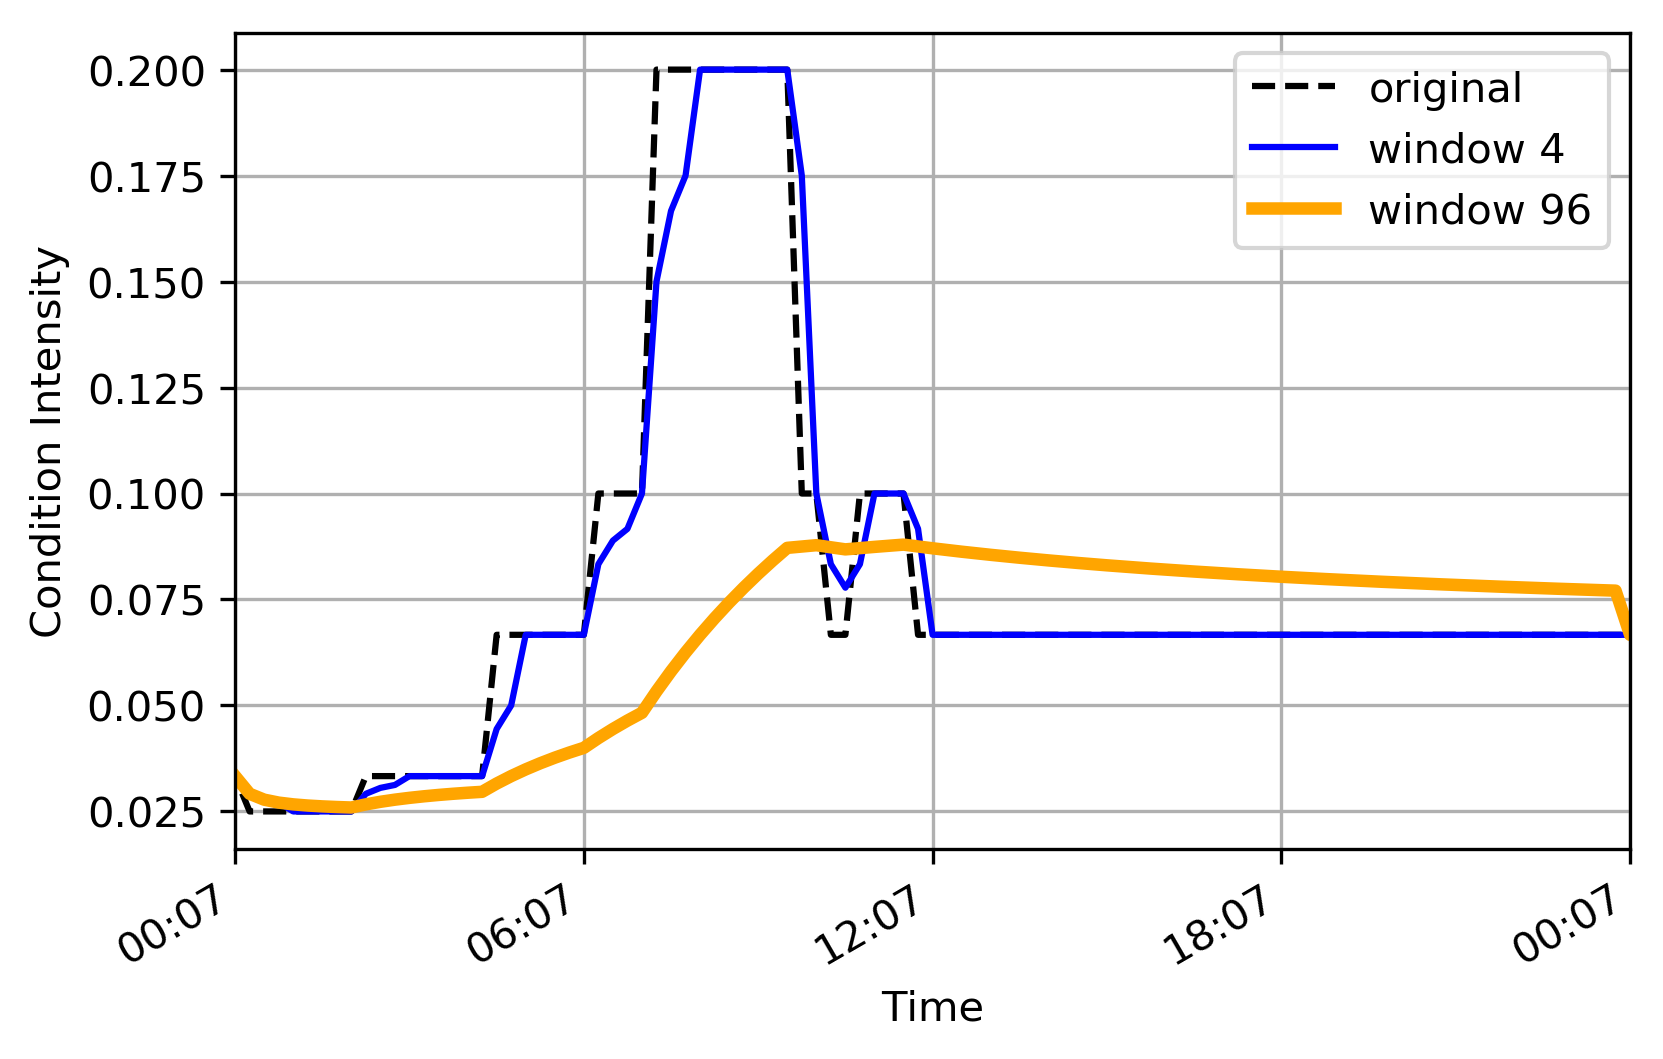
\includegraphics[width=0.5\textwidth]{figures/pocampo_expanding.png}\label{pocampo_expanding}}
    \caption{Comparison of Rolling and Expanding windows 4 and 96 to original Northbound traffic in Pablo Ocampo}
    % \label{figure_autocorr_traffic_season}
\end{figure}

\begin{figure}[t] 
\centering
  \centering
  \scalebox{.65}{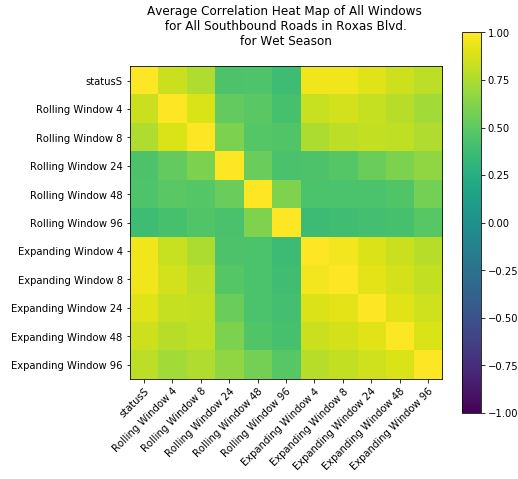
\includegraphics{figures/heatmap_roxas.JPG}}
  \caption{Average Correlation of Rolling and Expanding Mean to All Southbound Roads in Roxas Blvd.}
  \label{heatmap_roxas}
\end{figure}

Figure \ref{heatmap_roxas} shows the average correlation of southbound road segments of Roxas Boulevard per window size in relation to traffic for both rolling and expanding windows. On average, the original traffic has a strong relationship with rolling features having small window size, specifically window 4 with a correlation value of 0.7501. It is noticeable, however, that the strength of the relationship dwindles down as the window size increases. This reveals that although having a bigger window size means being able to capture various changes in traffic condition, it does not give importance to the most recent traffic conditions. Big changes in traffic conditions that occurred way back and may not have any effect on the current traffic are being considered. Thus, causing its misalignment to the original data. 

In the case of expanding windows, the strength of the relationship to the original traffic also decreases as the window size increases, albeit not so much as the rolling mean do. Looking into both graphs, the strength of the relationship given by window 4 for both rolling and expanding is distinctly stronger compared to the ones with larger window size. This might be because as mentioned earlier, traffic does not usually change significantly within a small window. Furthermore, a smaller window size means that its frequency of reverting back to the original value, making its generated value more accurate. Meanwhile, the farther from the past that it considers, the less it captures changes in traffic. This is shown in Figures \ref{pocampo_rolling} and \ref{pocampo_expanding}, where rolling and expanding at window 96 generalizes the high condition intensities into information that is no longer close to reality. Furthermore, the plodding decrease of correlation strength in expanding features as compared to rolling features is caused by limiting the number of windows that the feature grows to and considers and the restarting of its window size. Not limiting the window size growth of expanding features would produce values that are very far away from reality because it would consider every data from the previous days. It would contain values that consider data that are not relevant in predicting the future traffic.



























\pagebreak[4]
\section{Predicion Model Evaluation}

\subsection{Traffic-Only Model}
Traffic-Only Model implemented in DBN was first evaluated. 
As seen in Figure \ref{fig:tom_diff_feat_combi} the inclusion of the information about working days and peak hours for all road segments improved the performance of the model by only 22\% having originally an RMSE of 0.167 which improved to 0.113. As discussed earlier on the trend and patterns of traffic, though there is a difference between the trends of working days and non-working days, light and moderate traffic are most frequent in both trends in the majority of the road segments. This implies that the mean traffic condition intensity for both working and non-working days are similar. This similarity attributes to the small improvement in the prediction. Furthermore, including rolling and expanding window features for traffic significantly improved the prediction by around 53\%, from having an RMSE of 0.129 to 0.061 by window 4. Rolling and Expanding window features present a generalized information regarding the trend of the immediate past traffic. As discussed earlier, average traffic does not change significantly within a small window. Moreover, increasing the window size of both features As such, the performance of the model decreases as the window increases. 

\begin{figure}[!t]
  \centering
  \captionsetup{justification=centering}
  \scalebox{.65}{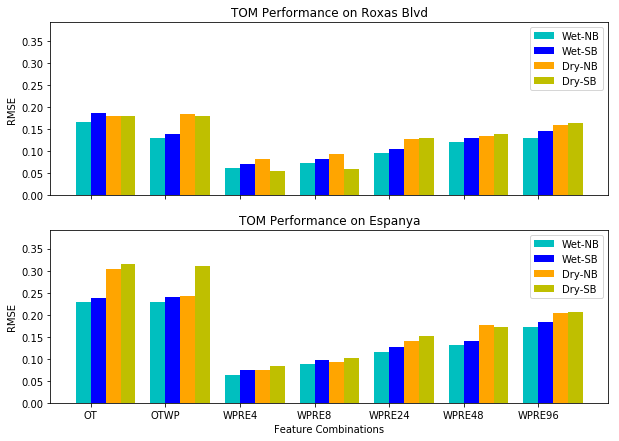
\includegraphics{tom_diff_feat_combi.PNG}}
  \caption{Comparison between performance of DBN TOM on Roxas Boulevard and Espana using different feature combinations}
  \label{fig:tom_diff_feat_combi}
\end{figure}

To evaluate if the model can successfully identify the trends present for each road segment, and its ability to predict its traffic, the performance of the model using OTWP or Original Traffic with the addition of work day and peak hours was observed. Results of this evaluation are illustrated in Figure \ref{fig:tom_feat_combi_road}. The model predicted the southbound traffic of España during the wet season quite well, having a mean RMSE of 0.095 compared to the other. However, this is because of the diversity of the southbound traffic of España during the wet season, having a moderate traffic congestion majority of the time. Given only data of the previous day’s traffic, and information on work day and peak hours, the model cannot easily model the sudden peaks and traffic reports on heavy traffic. Additionally, given the percentage of the report on heavy traffic congestion of the data, having only 10.584\% during the working days, and 0.301\% during the non-working days, the model lacks knowledge on modeling expected heavy traffic. 

\begin{figure}[!t]
  \centering
  \captionsetup{justification=centering}
  \scalebox{.55}{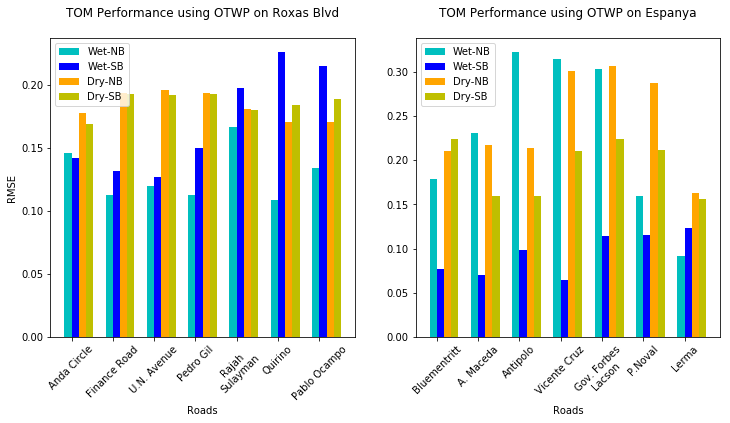
\includegraphics{tom_feat_combi_road.PNG}}
  \caption{Performance of DBN TOM on Roxas Boulevard and España using OTWP traffic feature combination}
  \label{fig:tom_feat_combi_road}
\end{figure}
 

Disrupted days refer to the period in time wherein the trend of traffic goes out of its normal trend. Traffic that goes out of its normal trend is most expected during days that have  heavy rainfall, or periods when typhoons are present. Figure \ref{fig:TOM_normal_disrption_pocampo_antipolo_wet} illustrates the prediction of TOM for traffic condition intensity for road segments of Pablo Ocampo and Antipolo during the wet season for the month of September. Normal trend includes the week of September 20 to 26, and the disrupted trend includes the week of September 6 to 12, both weeks include weekday and weekend. The period of disruption, specifically September 11 to 12, there are 40 and 56 instances of heavy rainfall, respectively. The actual traffic during the period of disruption transition from heavy traffic to to moderate traffic in just a small time interval, unlike normal transitions. The model successfully predicts the abrupt transition of low traffic to high traffic for both normal and disrupted periods. However, the model delays in predicting the abrupt transitions from high traffic to moderate traffic, and moderate traffic to moderately high traffic. These difficulty in prediction can be attributed to the few instances where these abrupt transitions are present. As seen, normal trends do not often include these abrupt transitions. 

\begin{figure}[!t]
  \centering
  \captionsetup{justification=centering}
  \scalebox{.65}{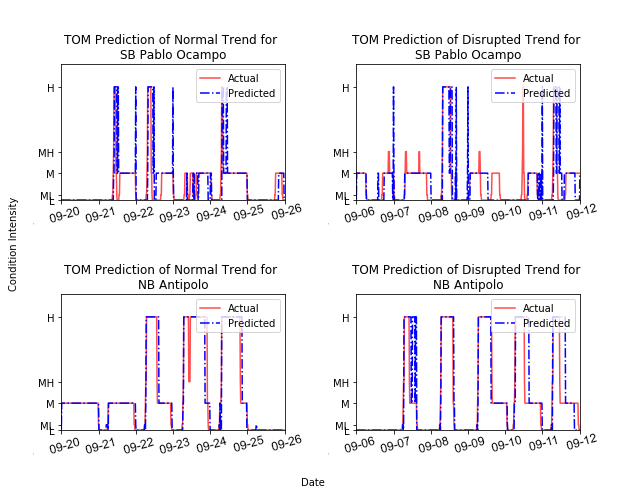
\includegraphics{TOM_normal_disrption_pocampo_antipolo_wet.PNG}}
  \caption{DBN TOM Prediction for Normal (left) and Disrupted (right) trends for Pablo Ocampo and Antipolo}
  \label{fig:TOM_normal_disrption_pocampo_antipolo_wet}
\end{figure}

Figure \ref{fig:rnn_dbn_tom_pocampo} illustrates the comparison of TOM implemented in RNN and DBN in predicting southbound traffic of Pablo Ocampo in the wet season. Results show that RNN performs better in predicting traffic than DBN. RNN could effectively predict traffic with just information on the mean of traffic 6 weeks ago, and traffic a day ago. Rolling and expanding window features that describe immediate past traffic could be removed, as it could add more complexity in predicting traffic, or it could have been a redundant feature, as shown in the small difference between not using these features, and using these features. Moreover, RNN predicts disruptions, and sudden traffic changes better than DBN as illustrated in Figure \ref{fig:RNN_TOM_normal_disrption_pocampo_antipolo_wet}. The figure clearly illustrates RNN's effective predictions for sudden traffic changes when traffic peaks and heavy traffic condition intensity is most expected, even with the small prior knowledge on heavy traffic unlike DBN. 

\begin{figure}[!t]
  \centering
  \captionsetup{justification=centering}
  \scalebox{.65}{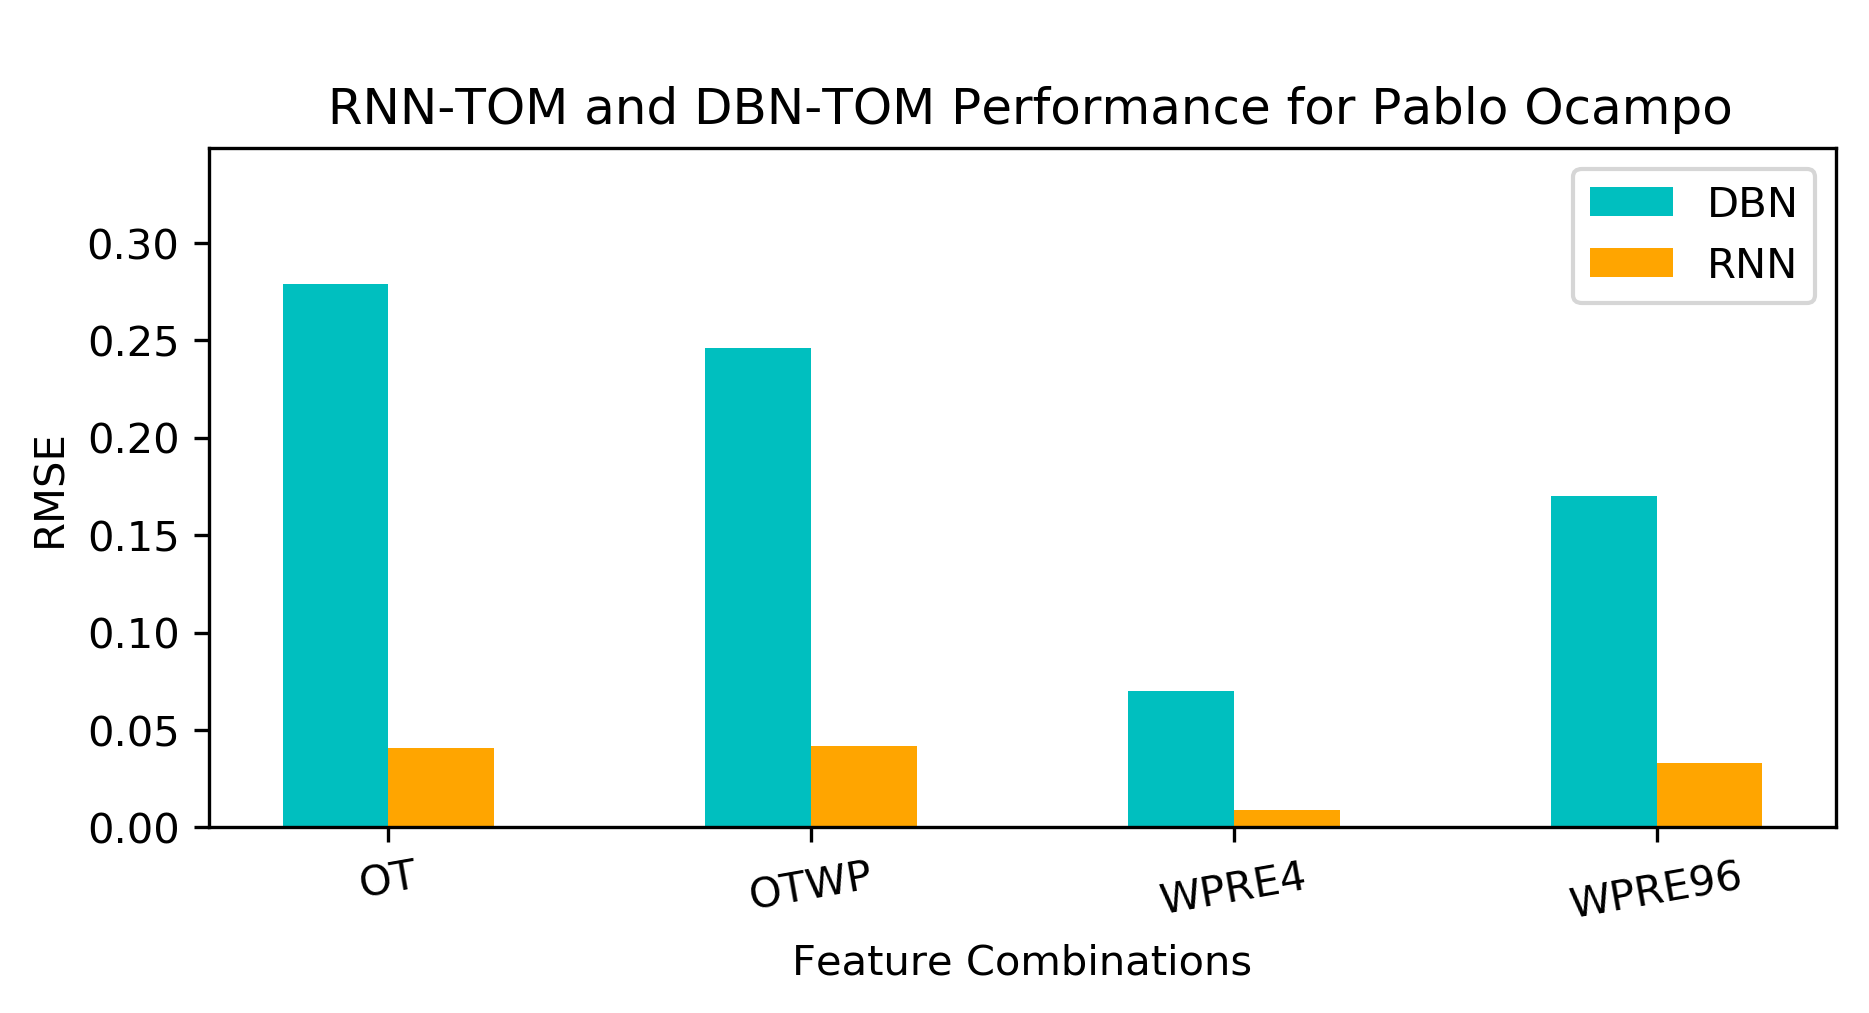
\includegraphics{rnn-dbn-tom-pocampo.PNG}}
  \caption{Comparison between RNN TOM and DBN TOM}
  \label{fig:rnn_dbn_tom_pocampo}
\end{figure}

\begin{figure}[!t]
  \centering
  \captionsetup{justification=centering}
  \scalebox{.65}{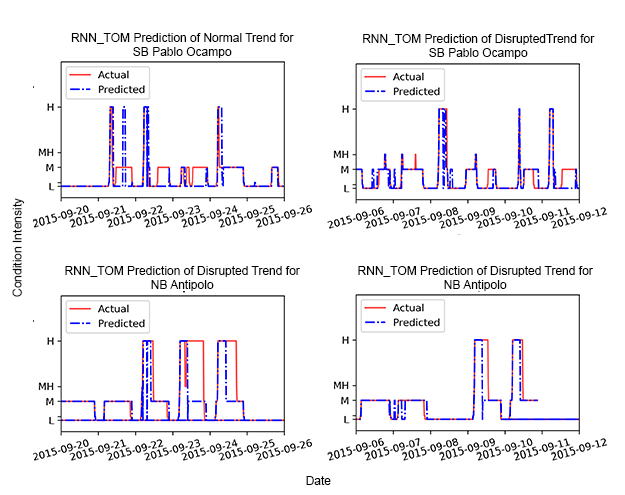
\includegraphics{RNN_TOM_normal_disrption_pocampo_antipolo_wet.PNG}}
  \caption{RNN TOM Prediction for Normal (left) and Disrupted (right) trends for Pablo Ocampo and Antipolo}
  \label{fig:RNN_TOM_normal_disrption_pocampo_antipolo_wet}
\end{figure}


\subsection{Weather-Only Model}
Given the weak relationship between weather variables with traffic, the model could only predict traffic about 80 to 84\% after using weather variables for input as compared to using past traffic that can predict traffic by 90\%. Furthermore, the model’s performance did not improve significantly with different combinations (see Figure \ref{fig:wom_diff_feat_combi}) of weather variables having changes in error ranging from only 0.001 to 0.003. Weather variables were found to have a low correlation, ranging from 0.01 to 0.3 with respect to the traffic condition intensity. Including and removing redundant variables, and other low correlated variables did not have a significant effect on the prediction. 

\begin{figure}[!t]
  \centering
  \captionsetup{justification=centering}
  \scalebox{.55}{\includegraphics{wom_diff_feat_combi.PNG}}
  \caption{Performance of DBN WOM on Pablo Ocampo and Antipolo using weather feature combinations}
  \label{fig:wom_diff_feat_combi}
\end{figure}


Figure \ref{fig:wom_feat_combi_roads} illustrates the performance of WOM following OW feature combination for all road segments of España and Roxas Blvd. For predicting Roxas Blvd road segments using WOM, the model predicts traffic better during the wet season. Additionally, WOM predicts northbound well for most road segments in Roxas Blvd during the wet season. Northbound traffic for these roads is less diverse, meaning that traffic majorly consists of low to moderate traffic, with only a few instances of abrupt transitions from these conditions to heavy traffic. Given these, WOM could not learn the pattern of these transitions given the few instances. In predicting the traffic of Roxas Blvd road segments during the dry season, the WOM could only predict 70\% of the traffic for the northbound of all road segments except Pedro Gil having an average RMSE of 0.250. 

As for predicting España Road segments using WOM, the model predicts southbound traffic of all roads during the wet season better. The WOM got an average RMSE of 0.329 in predicting northbound traffic for road segments Bluementritt to P. Noval, compared to predicting its southbound counterpart having an average RMSE of 0.116. Like Roxas Boulevard road segments, the southbound traffic of España road segments is less diverse, consisting mostly of low to moderate traffic.

For both roads of Roxas Boulevard and Espana, WOM could better predict the bound of a road segment with less diverse traffic, in which instances where traffic abruptly transitions to another traffic condition is not present. Moreover, WOM cannot predict fully traffic during the dry season, wherein weather, most especially rainfall, is less expected that can affect traffic fully. 


\begin{figure}[!t]
  \centering
  \captionsetup{justification=centering}
  \scalebox{.55}{\includegraphics{wom_feat_combi_roads.PNG}}
  \caption{Performance of DBN WOM using OW weather feature combination for all road segments}
  \label{fig:wom_feat_combi_roads}
\end{figure}

Given only temporal information and the weather variables to predict the current traffic condition intensity, and adding the fact that there is a small distribution of moderately high to high traffic in the data, the model could only predict low to moderate traffic successfully. Figure \ref{fig:WOM_normal_disrption_pocampo_antipolo_wet} illustrates the prediction of WOM for traffic condition intensity for road segments of Pablo Ocampo and Antipolo during the wet season for the month of September. WOM, however, predicted the transition of traffic from Low Traffic to either moderately low and moderate traffic well. WOM could predict the length of consistent traffic for both normal and disrupted periods. 

\begin{figure}[!t]
  \centering
  \captionsetup{justification=centering}
  \scalebox{.65}{\includegraphics{WOM_normal_disrption_pocampo_antipolo_wet.PNG}}
  \caption{DBN WOM Prediction for Normal (left) and Disrupted (right) trends for Pablo Ocampo and Antipolo}
  \label{fig:WOM_normal_disrption_pocampo_antipolo_wet}
\end{figure}

Figure \ref{fig:rnn_dbn_tom_pocampo} illustrates the comparison of WOM performance implemented in RNN and DBN in predicting southbound traffic of Pablo Ocampo in the wet season. Much like TOM, RNN outperforms DBN and effectively predicted traffic with just information on weather variables. However, much like DBN TOM, the differences in performance between AW, ACW, and CW feature combinations is significantly small. Even with the ability to extract temporal information on a time series, it cannot effectively extract the patterns between weather and traffic. Figure \ref{fig:RNN_WOM_normal_disrption_pocampo_antipolo_wet} illustrates prediction generated by RNN WOM for both normal and disrupted periods. Comparing the performance of DBN WOM, RNN WOM did predict more instances of traffic than the latter. It is important to note that RNN depends on patterns present in time series, such as seasonality, trends, and the like. However, weather does not strongly follow any trend. Using RNN to extract the relationship between traffic and weather may not be effective. Possibly, RNN needs more time-series information. 

\begin{figure}[!t]
  \centering
  \captionsetup{justification=centering}
  \scalebox{.65}{\includegraphics{RNN_WOM_normal_disrption_pocampo_antipolo_wet.PNG}}
  \caption{RNN WOM Prediction for Normal (left) and Disrupted (right) trends for Pablo Ocampo and Antipolo}
  \label{fig:RNN_WOM_normal_disrption_pocampo_antipolo_wet}
\end{figure}

\subsection{Fusion Analysis}
In analyzing the effectiveness of including weather as a factor in predicting traffic, the road segments which are strongly correlated with weather variables, and are more dynamic are selected in further analysis. These roads are southbound of Pablo Ocampo and northbound of Antipolo. The final results displayed are the average of the results of these two road segments.

\begin{table}[!t]
\begin{tabular}{|l|r|r|r|r|r|r|}
\hline
\multirow{2}{*}{\begin{tabular}[c]{@{}l@{}}Fusion \\ Techniques\end{tabular}} & \multicolumn{2}{c|}{\textbf{OTWP + OW}}                                & \multicolumn{2}{c|}{\textbf{WPRE 4 + OW}}                              & \multicolumn{2}{l|}{\textbf{WPRE 96 + OW}}                             \\ \cline{2-7} 
                                            & \multicolumn{1}{c|}{\textbf{RMSE}} & \multicolumn{1}{l|}{\textbf{MAE}} & \multicolumn{1}{c|}{\textbf{RMSE}} & \multicolumn{1}{l|}{\textbf{MAE}} & \multicolumn{1}{l|}{\textbf{RMSE}} & \multicolumn{1}{l|}{\textbf{MAE}} \\ \hline
\textbf{DBN TOM}             & 0.314                              & 0.148                             & 0.084                              & 0.011                             & 0.234                              & 0.090                             \\ \hline
\textbf{DBN WOM}             & 0.328                              & 0.149                             & 0.328                              & 0.149                             & 0.328                              & 0.149                             \\ \hline
\textbf{RNN TOM}             & 0.092                              & 0.183                             & 0.000                                 & 0.000                               & 0.045                              & 0.072                             \\ \hline
\textbf{RNN WOM}             & 0.147                              & 0.186                             & 0.147                              & 0.186                             & 0.147                              & 0.186                             \\ \hline
\textbf{DBN FF}                 & 0.322                              & 0.154                             & 0.092                              & 0.017                             & 0.277                              & 0.114                             \\ \hline
\textbf{RNN FF}                 & \textbf{0.078}                     & \textbf{0.101}                    & 0.077                              & 0.119                             & 0.078                              & 0.118                             \\ \hline
\textbf{DBN DF}                & 0.312                              & 0.140                             & 0.024                              & 0.003                             & 0.196                              & 0.006                             \\ \hline
\textbf{RNN DF}                & 0.072                              & 0.145                             & \textbf{0.038}                     & \textbf{0.086}                    & \textbf{0.063}                     & \textbf{0.125}                    \\ \hline
\textbf{WA DF}                 & 0.620                              & 0.618                             & 0.418                              & 0.405                             & 0.510                              & 0.504                             \\ \hline
\end{tabular}
\caption{Comparison between Prediction Models and Fusion Models}
\label{table:fusion_results}
\end{table}

In evaluating the DBN model, fusing traffic and weather at the decision level improved the prediction of TOM from an RMSE of 0.084 to 0.024, improving about 71\%. The performance of DBN in fusing data at the feature level was not far from the decision fusion model, only having a difference in RMSE of only 0.019. Predicting traffic considering both traffic and weather at the same time may weigh down the prediction of traffic because of the influence of weather. As discussed in early analysis of the weather data, it was found that weather variables do not have a derivable relationship with traffic. Adding weather features together with traffic adds more complexity to the model, adding more insignificant patterns to the learning, decreases the performance of the model to predict traffic. On the other hand, in fusing at the decision level, the traffic predicted by TOM does not have influence with weather, thus, minimizing the weights in predicting traffic. 


\begin{figure}[!t]
  \centering
  \captionsetup{justification=centering}
  \scalebox{.65}{\includegraphics{dbn_comp_pocampo.PNG}}
  \caption{Comparison of DBN models in predicting the southbound of Pablo Ocampo for the wet season}
  \label{fig:dbn_comp_pocampo}
\end{figure}

Figure \ref{fig:dbn_comp_pocampo} illustrates the differences of performance between DBN models, including decision and feature fusion DBN models that used predictions by the DBN prediction models. Including weather as a factor in predicting traffic improved the final predicting as seen in the results of fusing in the decision level. This improvement is significantly evident in the performance of the model after using predictions of TOM and WOM that used OTWP traffic features, and OW weather features, respectively. The prediction improved by 71\%, from having an RMSE of 0.084 to 0.024. As for using predictions of TOM and WOM that used WPRE4 traffic features and OW weather features, the predictions improved by 16\%. A reason behind only the small improvement is because of the consideration of rolling and expanding features at window 96, or within the current day. The window may have consisted instances of disruption that may have been generalized by the averaging traffic within 96 windows. Additionally, there is a small number of instances of heavy traffic that assists the rolling and expanding features in generalizing the traffic within said window. 


\begin{figure}[!t]
  \centering
  \captionsetup{justification=centering}
  \scalebox{.65}{\includegraphics{rnn_comp_pocampo.PNG}}
  \caption{Comparison of RNN models in predicting the southbound of Pablo Ocampo for the wet season}
  \label{fig:rnn_comp_pocampo}
\end{figure}

Figure \ref{fig:rnn_comp_pocampo} illustrates the differences of performance between RNN models, including decision and feature fusion RNN models that used predictions by the RNN prediction models. 
The difference in performance between the different feature combinations, and models were significantly small, having little to no changes in the performances. As discussed earlier, RNN could efficently predict traffic with only information on the mean of the past traffic, and instance of traffic a day before. These information already presents sufficient time-series characteristics, that adding more features may not be too significant in improving the performance. Much like DBN, the RNN DEI-DEO fusion model performed better than the RNN DEI-DEO model. However, the difference between the two performances are small because of the little significance weather features present in predicting traffic. However, both fusion models mostly improves the traffic prediction that did not consider weather. The prediction only improved by 2\%. However, comparing the performances of the RNN models with the DBN models, the RNN models outperformed the latter by 70\%. DBN-TOM had an RMSE of 0.314, whereas RNN-TOM had an RMSE of 0.041. DBN-Decision fusion model had an RMSE of 0.312, while RNN-Decision fusion model had an RMSE of 0.072. RNN models significantly outperforms DBN models. 

WA performed the worse of all fusion techniques, generating an RMSE of 0.512 to 0.620, as compared to the other techniques. WA, much like the other techniques, significantly improved as rolling and expanding windows were considered. Because the predictions come closer to the truth once rolling and expanding window features are considered, WA comes close as well. However, WA cannot effectively predict traffic that considers weather features. The inclusion of weather features may have added complexity in identifying the weights of the algorithm, and have added more weight in averaging two predictions, rather than improve it. WA considers the outlier and generates an inaccurate prediction. Because of such performance, WA is not considered in further experiments. The farther one prediction is to the other, the farther the outlier is away from the other, the more difficulty WA goes through in fusing decisions.  

A noticeable behavior is RNN outperformed the other fusion techniques. RNN has at least 74\% less error than DBN and WA. RNN is implemented as an LSTM, or a long short-term memory, compared to DBN which is implemented as a regressor and a classifier. Because of RNN’s power of long short-term memory, it can use their internal memory to process a sequence of inputs, successfully extracting ordered patterns. However, as mentioned earlier, RNN could not improve the prediction of the RNN TOM model. However, the fusion model in DBN improved the TOM and WOM's prediction because of the RBMs implemented into the network that can extract pattern from the data. 

The implemented model could predict normal trends of traffic. However, disrupted traffic trends defined in the discussion of the traffic and weather data cannot be accurately predicted. A reason behind the difficulty in prediction is the small number of instances of disruption in the training dataset. There is only a small number of instances of moderately heavy to heavy traffic within the wet season of the training dataset. Another reason may be because of the instances when disruptions in weather were present until the weekends when traffic is least expected. For example, for September 11 to 14 when typhoon Ineng was present, extends from a Friday until Sunday. The model also has a difficulty in predicting traffic using only weather features because of the weak relationship between these variables. For visualization purposes, the final prediction of traffic condition  intensity of Pablo Ocampo and Antipolo is illustrated in Figure \ref{fig:final_prediction}.

\begin{figure}[!t]
  \centering
  \captionsetup{justification=centering}
  \scalebox{.55}{\includegraphics{RNN_final_prediction.PNG}}
  \caption{Final Prediction generated by RNN Feature Fusion model for Normal (left) and Disrupted (right) trends for Pablo Ocampo and Antipolo using DBN Decision Fusion}
  \label{fig:final_prediction}
\end{figure}































\subsection{Sensitivity Analysis}
To analyze the effectiveness of including weather as a factor in predicting traffic, the southbound traffic of Pablo Ocampo were selected. The final results displayed are the average of the results of these two road segments.

\subsubsection{Traffic-Only Model}

Evaluation of the sensitivity of TOM is illustrated in Figure \ref{fig:TOM_sensitivity}. It has been discussed in the early sections in evaluating TOM that the inclusion of work day and peak hour variables result in a 22\% improvement in performance. In considering the working day and peak hour information, the removal of temporal information decreased the performance from 3.9 to 8.6\%. Not one temporal information increased the accuracy. However, the removal of temporal information without considering the working day and peak hour information increased the performance, but only by 0.4 to 3.1\%. This change in accuracy can be because of the model being given more complexity as more traffic features that are not exactly strongly connected with each other. An example of this is the variable \textit{Day}. This variable decreased the accuracy the most out of all temporal information, having a decrease in accuracy of 8.6\%. Other included traffic features do not depend on the day of the month. Hence, the significant decrease in accuracy. As for other temporal information variables, \textit{Month, Hour and Minute, and Day of the Week} may describe traffic with the support of other traffic features. However, traffic disruptions and traffic trend changes occur. In the case of \textit{Month}, noticeable traffic in a week in a month does not necessarily mean that it will be traffic the whole month. In the case of \textit{Hour and Minute}, traffic this hour during a Friday does not necessarily mean it will be traffic that particular hour and minute during a Saturday, Sunday or even a Monday. In the case of \textit{Day of Week}, given the number of records of heavy traffic that working day and peak hour information is derived from, day of week which depends on working day and peak hour, cannot effectively describe traffic. Moreover, in considering traffic features that effectively describes its immediate past traffic condition, such as using rolling and expanding window features, adding temporal information adds more complexity to the model such that it contradicts the findings of these traffic features with the patterns extracted by the temporal information variables. This is evident by the significant increase in accuracy by 4\% when using rolling and expanding window features at window 96, and small increases and decreases in accuracy from 0.4\% to 3.1\% at window 4, as compared to having no rolling and expanding window features. 

\begin{figure}[!t]
  \centering
  \captionsetup{justification=centering}
  \scalebox{.35}{\includegraphics{TOM_sensitivity.PNG}}
  \caption{Sensitivity of TOM with different feature combinations}
  \label{fig:TOM_sensitivity}
\end{figure}

Looking into the effect of the past traffic feature when used with working day and peak hour, removing mean traffic 6 weeks ago significantly decreased the accuracy of the prediction by 12.2\%. Moreover, the same decrease of accuracy was observed when past traffic features excluding working day and peak hour, and all temporal information was removed. Using only mean traffic 6 weeks ago as a past traffic feature, without the consideration of working day and peak hour, increased the accuracy by 15.4\%. Meanwhile, the accuracy decreased by 4.7\% to 2.2\% after considering working day and peak hour. As discussed, working day and peak hour may have added complexity in predicting traffic using traffic features with patterns that may go against patterns of working day and peak hour. Moreover, given the small records of heavy traffic in the data which working day and peak hour extracts, these traffic features cannot describe traffic as much as the mean traffic 6 weeks ago, and traffic a day ago. Hence the significant increase in accuracy in removing working day and peak hour. Comparing the difference between the changes in accuracy between using mean traffic 6 weeks before, and traffic a day before, the accuracy significantly changed in considering the mean traffic 6 weeks ago. This show that this feature has great importance in predicting traffic. However, with the inclusion of rolling and expanding window features which describes the traffic of the immediate past, using the mean of the traffic 6 weeks before or traffic a day before does not significantly affect the accuracy of the prediction. This can be because of the relationship between the window features with the current traffic, which outperforms the patterns extracted by the mean traffic 6 weeks before and traffic a day before. 


\subsubsection{Weather-Only Model}
Evaluation of the sensitivity of WOM is illustrated in Figure \ref{fig:WOM_sensitivity}. As discussed in the evaluation of the WOM with the different combination of the weather features, the varying combinations did not go far from the results of using all weather features, from having a differnce in RMSE from 0.001 to 0.003. The strength of the correlation between weather features to traffic were weak that it removing any weather feature did not significantly effect the prediction. Therefore, the change in accuracy ranges from 0 to 2.7\%. However, using the weather feature that has the highest correlation with traffic between other weather variables, excluding redundant variables, did improve the prediction but only by 1.5\%. This proves that the strength of the relationship between weather and traffic is important to understand to achieve better prediction. 

\begin{figure}[!t]
  \centering
  \captionsetup{justification=centering}
  \scalebox{.45}{\includegraphics{WOM_sensitivity.PNG}}
  \caption{Sensitivity of WOM with different feature combinations}
  \label{fig:WOM_sensitivity}
\end{figure}

The effect of temporal information to predicting traffic using all weather features was also evaluated, as illustrated in Figure \ref{fig:WOM_sensitivity}. WOM uses only weather variables and temporal information to predict traffic. Of all the features, the closest to describe traffic are the temporal information features (e.g. Month, Day, Hour, Minute, Day of the Week). As such, the prediction decreased as temporal information was removed. However, as mentioned in discussing the sensitivity of the Traffic-Only Model features, temporal information without the support of working day and peak hour flags cannot effectively describe traffic. Hence, the small decrease in accuracy as temporal information was removed. Moreover, using information on the \textit{Day of Week} increased the accurcy by 6.4\%. Using information on \textit{Month, Day, Hour and Minute} alone descreased the accuracy, as traffic does not strongly depend on these information, especially in working days and peak hours. 


\subsubsection{Decision Fusion Model}

\begin{figure}[!t]
  \centering
  \captionsetup{justification=centering}
  \scalebox{.45}{\includegraphics{pm1-pm2-df-changes.PNG}}
  \caption{Change in performance in different feature combinations}
  \label{fig:pm1-pm2-df-changes}
\end{figure}

To evaluate the effectiveness of including weather in predicting traffic, the performance of the fusion model is compared with the performance of the Traffic-Only model for each feature combination. The performances of these models was based from the results illustrated in Table \ref{table:fusion_results}. 

As discussed in the Fusion Analysis, considering the weather prediction in fusing at decision level using WPRE96 feature combination resulted in a 16.2\% improvement in performance. However, in evaluating the performance of the weather in predicting traffic, weather only contributed about 23\% of the prediction after getting the difference between the performance between TOM and DEI-DEO fusion model, and dividing it by the max of the two. Accuracy significantly improved once window features at window 4 and 96 were considered. Though the difference between TOM and WOM in these feature combinations are far, from an RMSE of 0.084 in TOM to 0.328 in WOM, WOM played as a contributing factor in predicting traffic, achieving the increase in accuracy from 16.2\% to 71.4\%. 

As mentioned in earlier discussions, traffic data mostly comprises of moderate traffic condition intensity reports. Moreover, most road segments experience light to moderate traffic with few instances of disruptions, most of the day. Additionally, instances where there is a disruption in weather in which traffic is expected lies in weekends when traffic is least expected. Because of the lack of diverse data, it did not completely represent the relationship between weather and traffic, thus resulting in the small weight in prediction. 